\documentclass[12pt]{amsart}
\usepackage{fullpage,booktabs, graphicx,psfrag,amsmath, amssymb,amsthm, hyperref}

\input defs.tex




\title{A shape theorem for exploding sandpiles}
\author{Ahmed Bou-Rabee}

\begin{document}

	
	\begin{abstract}
		We study scaling limits of exploding Abelian sandpiles using ideas from percolation and front propagation in random media. 
		We establish sufficient conditions under which a limit shape exists and show via a family of counterexamples that convergence may not occur in general. A corollary of our proof is a simple criteria for determining if a sandpile is explosive; this 
		strengthens a result of Fey, Levine, and Peres (2010). 
		
		
	\end{abstract}
\maketitle



\section{Introduction}
\subsection{Overview}
We consider the Abelian sandpile growth model on the integer lattice. Start with a {\it background} of indistinguishable chips, $\eta: \Z^d \to \Z$, add $n$ chips at the origin, 
and attempt to {\it stabilize} via {\it parallel toppling}:
\begin{equation} \label{eq:parallel_toppling}
\begin{aligned}
v_{t+1} &= v_{t} + 1 \{ s_{t} \geq 2 d \} \\
s_{t+1} &= s_{t} + \Delta (v_{t+1} - v_{t}), 
\end{aligned}
\end{equation}
where $\Delta v(x) = \sum_{y\sim x} (v(y) - v(x))$ is the Laplacian on $\Z^d$, $v_0 = 0$ is the initial {\it odometer}, and $s_0 = \eta + n  \delta_0$ is the starting sandpile. We say $s_0$ is {\it stabilizable} if there is $T < \infty$ so that 
$v_{t} = v_{T}$ for all $t \geq T$. A background is {\it robust} 
if $\eta + n  \delta_0$ is stabilizable for all $n \geq 1$, and otherwise 
is {\it explosive}. When $s_0 = \eta + n  \delta_0$ is not stabilizable, it is explosive and the infinite sequence $\{s_t\}_{t \geq 0}$ is an {\it exploding} sandpile. See Figures \ref{fig:exploding_random1} and \ref{fig:exploding_random2}.




Fey, Levine, and Peres coined these notions in \cite{fey2010growth} (see also \cite{fey2005organized}) and provided sufficient conditions for determining if a background is explosive or robust: backgrounds $\eta \leq (2d-2)$ are always robust, but otherwise can be robust or explosive, depending on the arrangement of sites with $(2d-1)$ chips. In fact, they showed that if $\eta \leq (2d - 2)$, not only 
is the background robust, but if $n$ chips are added to the origin of such $\eta$, the diameter of the set of sites which topple grows like $n^{1/d}$. 


\begin{figure}[b!]
	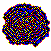
\includegraphics[width=0.2\textwidth]{Figures/iid_background/2D_seq/51.png}
	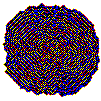
\includegraphics[width=0.2\textwidth]{Figures/iid_background/2D_seq/101.png}
	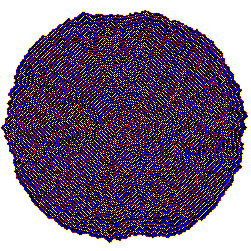
\includegraphics[width=0.2\textwidth]{Figures/iid_background/2D_seq/251.png}
	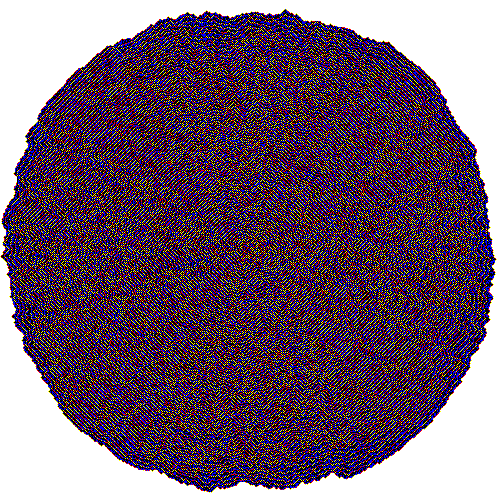
\includegraphics[width=0.2\textwidth]{Figures/iid_background/2D_seq/501.png}
	\caption{$s_t  1\{ v_t > 0 \}$ for $\eta \sim \mbox{Bernoulli}(3,2,1/2)$ and $t = 50, 100,250,500$.
		The color white denotes sites which haven't toppled yet, otherwise white, yellow, red, blue, and black correspond to values $0, 1,2,3, (\geq 4)$.
	}  \label{fig:exploding_random1}
\end{figure}




Pegden and Smart used this bound together with the theory of viscosity solutions to show that the terminal odometer
for $n  \delta_0$, after a rescaling, converges to the solution of a fully nonlinear elliptic PDE \cite{pegden2013convergence}.
This breakthrough then led to an explanation for the patterns which appear in two-dimensional sandpiles \cite{pegden2020stability, levine2016apollonian, levine2017apollonian}. Recently, the author used stochastic homogenization methods to extend convergence to all initial backgrounds which are stationary, ergodic, and bounded from above by $(2 d - 2)$ \cite{bou2019convergence}. 

\begin{figure}[t]
	
\includegraphics[width=0.2\textwidth]{Figures/iid_background/2D/p_14.png}
	
\includegraphics[width=0.2\textwidth]{Figures/iid_background/2D/p_12.png}
	
\includegraphics[width=0.2\textwidth]{Figures/iid_background/2D/p_34.png} \\
	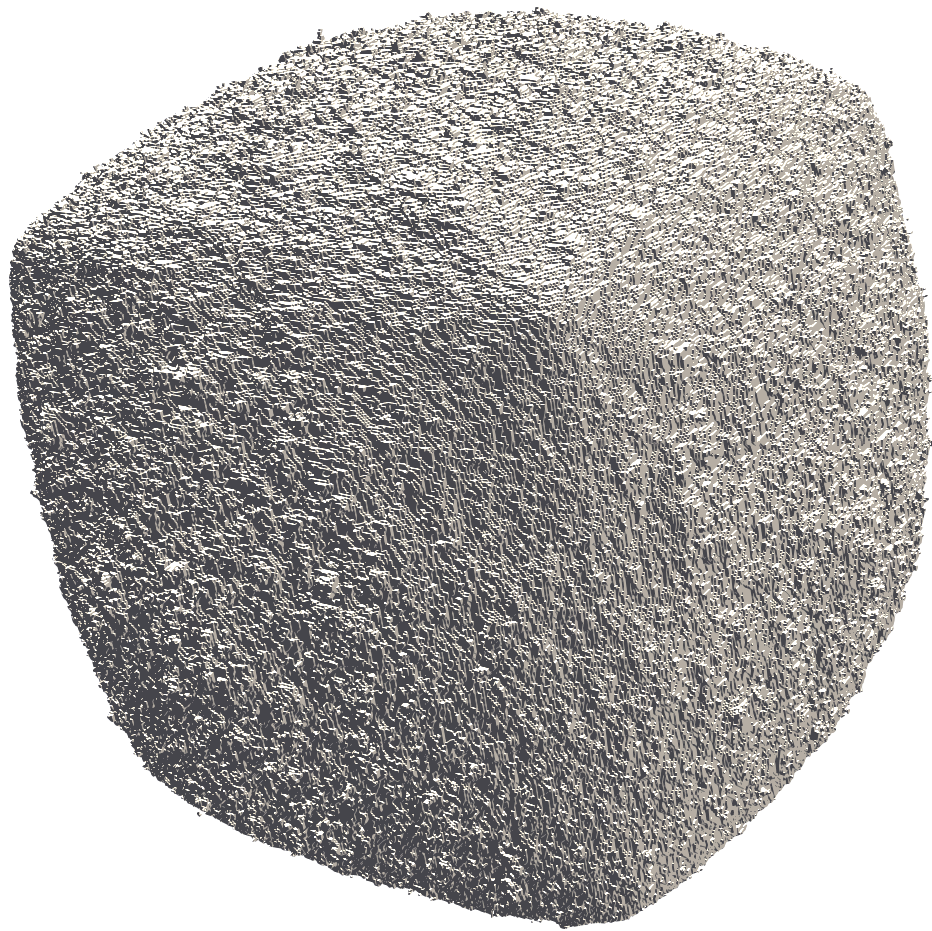
\includegraphics[width=0.2\textwidth]{Figures/iid_background/3D/p_34.png}
	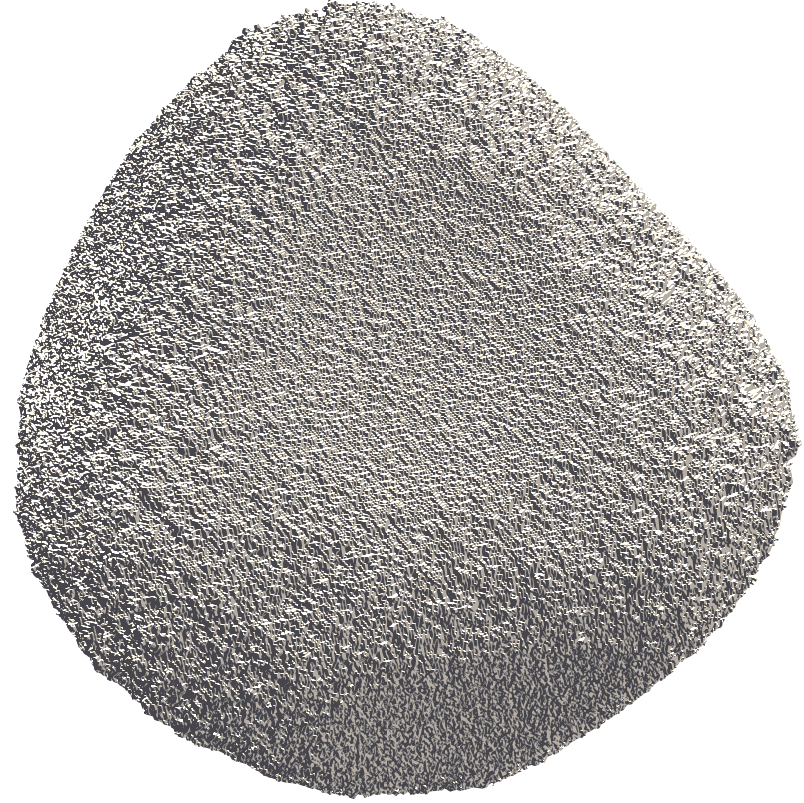
\includegraphics[width=0.2\textwidth]{Figures/iid_background/3D/p_12.png}
	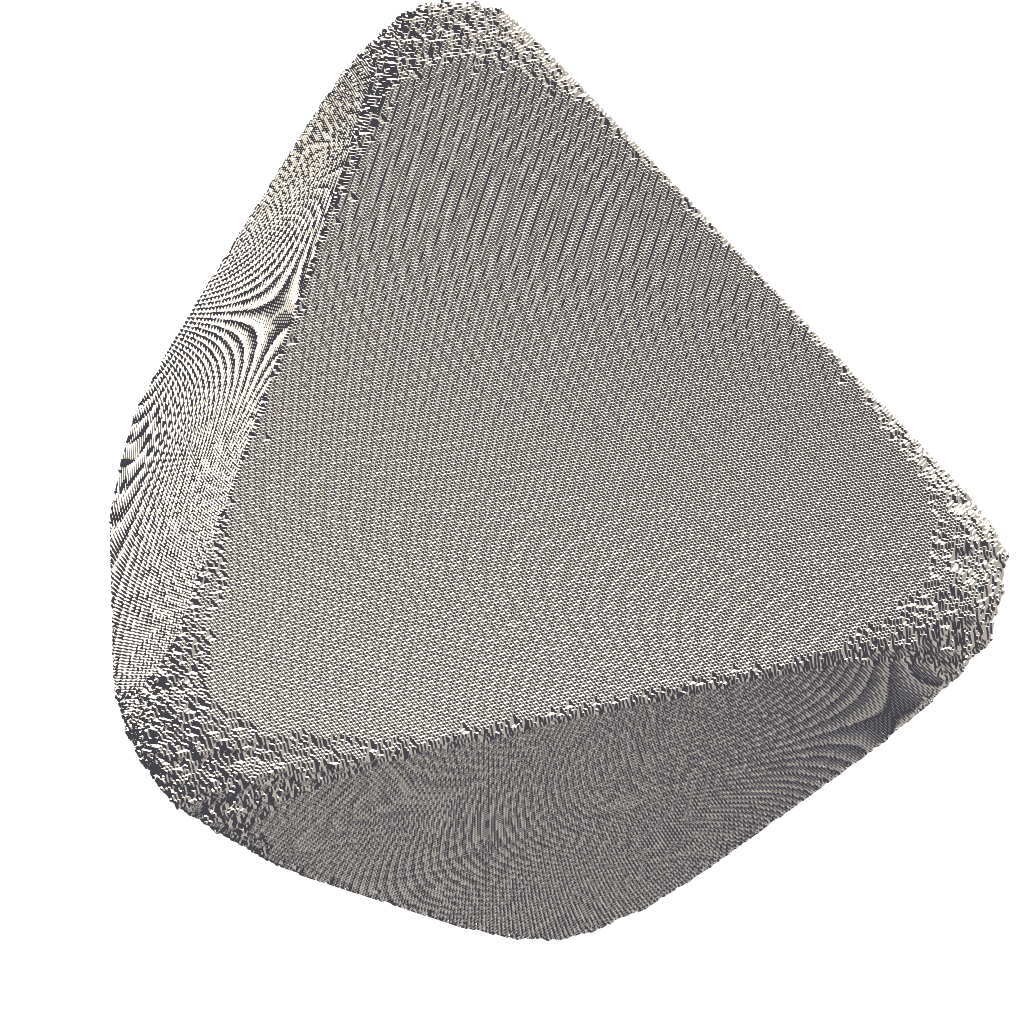
\includegraphics[width=0.2\textwidth]{Figures/iid_background/3D/p_14.png}
	\caption{Snapshot of the support of an exploding sandpile $1 \{v_t > 0\}$  for $\eta \sim \mbox{Bernoulli}(2 d - 1, 2d - 2,p)$
		the first time it exits a box of side length $500$. The top row is $d = 2$ and the bottom $d = 3$. 
		From left to right, $p = 1/4, 1/2, 3/4$.}  \label{fig:exploding_random2}
\end{figure}


These results explain the phenomena of {\it scale-invariance} in sandpiles which have a {\it compact}, $n^{1/d}$, growth rate --- large, compact-growth sandpiles look like high-resolution versions of smaller sandpiles. Simple models of growth are of interest to the mathematics and physics communities ---  see, for example, \cite{dhar2013sandpile,diaconis1991growth, gravner1998cellular, packard1985two} and the references therein. The Abelian sandpile in particular has a rich history,  \cite{liu1990geometry, dhar1999abelian,le2002identity, ostojic2003patterns,  redig2005mathematical,fey2008limiting, holroyd2008chip, fey2009stabilizability, levine2009strong, levine2010sandpile, paoletti2013deterministic,levine2017laplacian, jarai2018sandpile,  klivans2018mathematics, hough2019sandpiles, aleksanyan2019discrete, lang2019harmonic, hough2019cut,chen2020laplacian, melchionna2020sandpile, alevy2020limit}. 


In this paper, we study limit shapes of sandpiles in the explosive regime. The techniques used differ fundamentally from the existing compact-growth theory. Indeed, as we will demonstrate, some explosive sandpiles (both random and deterministic) do not converge. On the other hand, compact-growth sandpiles essentially always have limits --- the argument there is `soft' and applies in wide generality. Our proof below is quantitative and involves establishing specific, finite-scale estimates. We identify sufficient conditions under which exploding sandpiles converge to the level set of an asymmetric norm  --- much like in first-passage percolation  \cite{cox1981some} and threshold growth \cite{willson1978convergence, gravner1993threshold}.


\subsection{Main results}	
For expositional clarity, we consider one family of random, explosive backgrounds with limit shapes. The reader interested in generalizations may consult Section \ref{sec:generalization}. Suppose $d \geq 2$ and $\eta:\Z^d \to \Z$ is drawn from a product measure $\mathbf{P}$ with
\begin{equation}\label{eq:toy-eta-definition}
\begin{gathered}
0<p\leq1,\qquad
\nu_p=(1-p)\delta_{2d-2}+p\delta_{2d-1},\qquad
\mathbf P=\bigotimes_{x\in\Z^d}\nu_p,\\
\mathbf P(\eta(x)=2d-2)=1-p,\qquad
\mathbf P(\eta(x)=2d-1)=p\quad(x\in\Z^d)\,.
\end{gathered}
\end{equation}
Fey, Levine, and Peres showed the following.
\begin{theorem}[Proposition 1.4 in \cite{fey2010growth}]\label{prop:fey_levine_peres_explode}
	Let $\eta$ be as in \eqref{eq:toy-eta-definition}.  If $p > 0$, $\eta$ is explosive with probability 1. 
\end{theorem}
Fix $p > 0$ and denote the (almost surely finite) {\it explosion threshold} by
\begin{equation} \label{eq:first_explosion}
M_{\eta} :=  \min\{ n \geq 1 : \mbox{ $\eta + n  \delta_0$ is not stabilizable} \}. 
\end{equation} 
We prove that the support of the infinite sequence of parallel toppling odometers, $\{v_t\}_{t \geq 1}$, for the explosive sandpile $s_0 = \eta + M_{\eta}  \delta_0$ converges under rescaling. 
\begin{theorem} \label{theorem:limit_shape}
	Let $\eta$ be as in \eqref{eq:toy-eta-definition}. 
	There exists a convex domain $\mathcal{B}(p) \subset \R^d$ so that on an event of 
	probability 1, 
	\[
	| \{ \bar{v}_t > 0\} \triangle \mathcal{B}(p)| \to 0, 
	\]
	where $\bar{v}_t(x) := v_t([t x])$. 
\end{theorem}
In fact, we prove something stronger. Not only does the support of the explosion converge, 
but the rate at which the explosion spreads also converges. 


\begin{theorem} \label{theorem:convergence_of_time_constant}
	Let $\eta$ be as in \eqref{eq:toy-eta-definition} and let $T_{\eta}(x) := \min\{t \geq 1 : v_t(x) > 0 \}$. On an event of probability 1, the rescaled arrival times $\bar{T}_{\eta}(x) := n^{-1} T_{\eta}([ n x])$
	converge locally uniformly to $\mathcal{N}_{p}$, a continuous, convex, one-homogeneous function on $\R^d$. 
\end{theorem}
During our proof of Theorem \ref{theorem:convergence_of_time_constant}, we introduce a quantitative criterion for determining if a sandpile is explosive. The criterion asserts, roughly, that if a sandpile explodes quickly on a finite box, then it must do so on the entire lattice. 
We use this and a coupling with bootstrap percolation to extend the aforementioned Theorem \ref{prop:fey_levine_peres_explode}. 
\begin{theorem} \label{theorem:explosive}
For $d\geq2$, let $\nu$ be a probability measure on $\Z$ with $\nu(\{m\in\Z:m\geq d\})=1$ and $\nu(\{2d-1\})>0$. If $\beta:\Z^d\to\Z$ has law $\mathbf P=\bigotimes_{x\in\Z^d}\nu$, then $\beta$ is explosive with probability 1.
\end{theorem}



\subsection{Proof outline}
An exploding sandpile may be thought of as a heterogeneous, discrete reaction-diffusion equation. This perspective leads us to the literature for stochastic homogenization of reaction-diffusion equations \cite{zhang2020long, feldman2019mean, lin2019stochastic, armstrong2018stochastic, caffarelli2014counter, gravner2006random, ishii1999threshold, barles1998new, gravner1996first,gravner1993threshold, willson1978convergence}. These works suggest two methods of proof. The first, which we do not pursue, is {\it half-space propagation}---a limit shape can be completely described by those starting with a half-space initial condition---an early example of this technique appears in \cite{willson1978convergence}. 
Another method is to identify a subadditive quantity similar to the first-passage time, \cite{cox1981some}, which (directly or indirectly) describes the limit shape, then apply the subadditive ergodic theorem.


Our proof of Theorem \ref{theorem:convergence_of_time_constant} follows the second outline,
however, there are several hurdles to overcome. A fundamental one is the nonlinear diffusion of the sandpile. This nonlinearity can cause explosions to propagate irregularly. In fact, an arbitrary exploding sandpile may spread quickly in certain cells, but slowly in others, causing convergence to fail. We demonstrate an explicit family of counterexamples to that effect in Section \ref{sec:counterexample}. A major part of our argument is showing that this irregularity cannot happen if $\eta \geq (2 d - 2)$ and there are `enough' sites with $(2d - 1)$ chips. 

From now until Section \ref{sec:generalization}, take $\eta$ as in the statement of Theorem \ref{theorem:convergence_of_time_constant} and fix $p > 0$. We begin in Section \ref{sec:fast_explosions} by showing that explosions on $\eta$ spread quickly. This is done by establishing a high-probability bound on the `crossing-speed' of $\eta$ in a finite, but large cube and passing to a coarsened lattice. On the coarsened lattice, there is an infinite cluster of `good cubes' upon which explosions are guaranteed to spread quickly. We use this together with
large-deviations for the chemical distance of supercritical Bernoulli percolation to get
uniform, linear bounds on the arrival times. (This portion of the proof shares some similarities with 
Schonmann's argument for bootstrap percolation \cite{schonmann1992behavior}.)

At this stage, if the arrival times, $T_{\eta}$, were subadditive, we could apply the subadditive ergodic theorem
and conclude. However, $T_{\eta}$ is not, in general, subadditive: roughly, when an explosion
started at the origin reaches some site $x$ for the first time, it mixes up the background
and so cannot be compared directly to the explosion originating from $x$. 

We overcome this lack of subadditivity by shifting our focus to a related, but simpler process, 
the {\it last-wave}---an exploding sandpile where the origin is constrained to topple a fixed number of times.  In Section \ref{sec:last_wave}, we use the established regularity of explosions to show that the last-wave can be approximated by a quantity which is exactly subadditive, and hence converges. This can also be viewed as a shape theorem for a bootstrap percolation type process. 

The proof of Theorem \ref{theorem:convergence_of_time_constant} is completed in Section \ref{sec:proof_of_theorem} where we show that the last-wave is an approximation to the expanding front of an exploding sandpile. The argument for this is a deterministic comparison which requires $\eta \geq (2d - 2)$. Then, in Section \ref{sec:generalization}, we generalize Theorem \ref{theorem:convergence_of_time_constant} 
by presenting sufficient hypotheses under which a limit shape exists. We demonstrate some need of these hypotheses
by constructing a family of (random and deterministic) exploding sandpiles which fail to have a limit shape in Section \ref{sec:counterexample}. We conclude in Section \ref{sec:criteria} with a proof of Theorem \ref{theorem:explosive}. There we indicate explicit criteria 
for determining if a sandpile is explosive. 

\subsection*{Use of artificial intelligence}
The original paper (2021) was written by the author. This corrected edition was prepared while the paper was formalized in the Lean proof assistant. AI coding agents (Anthropic Claude and OpenAI GPT models, with DeepSeek and Mistral models for auxiliary proof search), directed by the author, found the corrections listed in the section ``Corrections to the published version'' and drafted the corrected statements, the new proofs and Remark~\ref{rem:sharp_planar_obstruction}. The author checked these.
Every numbered result of this edition and Remark~\ref{rem:sharp_planar_obstruction} is proved in Lean. Three cited results enter as explicit hypotheses: Theorem~1.1 of Antal and Pisztora~\cite{antal1996chemical}; Theorem~4.1 of Fey, den Boer and Redig~\cite{fey2008limiting} and the radius bound of Fey, Levine and Peres~\cite{fey2010growth}, which enter for Lemma~\ref{lemma:square_lower_bound} and Remark~\ref{rem:sharp_planar_obstruction}. Proposition~\ref{prop:explosion_criteria} is formalized for $d\geq2$, and Hypothesis~\ref{hyp:finite_range_of_dependence} is used in the form stated in this edition.
The author takes responsibility for the mathematical content and presentation of the paper.

\subsection*{Acknowledgments}
Thank you to Charles K. Smart for motivating, helpful discussions 
during this project. Thank you to Lionel Levine for several
inspiring conversations and for suggesting this question.  Thank you to Dylan Airey for asking if exploding sandpiles have a limit shape. 



\subsection*{Code}
Julia code which can compute the figures in this article is included in the arXiv upload and may be freely used
and modified.


\subsection*{Notation and conventions} 
\begin{itemize}
	\item Functions on $\Z^d$ are extended via nearest-neighbor interpolation to $\R^d$.  
	That is, if $f$ is a function on $\Z^d$, then for $x \in \R^d$, we define $f(x)$ to be $f([x])$ where $[x]$ is the nearest (breaking ties by picking the coordinate-wise minimum) point in $\Z^d$ to x. 
	\item $d$ will always refer to the dimension of the underlying space.
	\item $e_1, \ldots, e_d$ are the $d$ unit directions in $\Z^d$.
	\item $x_i = x \cdot e_i$ is the $i$th coordinate of vector $x$ and $\mathbf{x}_{d-i} = (x_{i+1}, \ldots, x_d)$.
	\item $|x|$ refers to the Manhattan norm and $|x|_{\infty}$ the $\ell_\infty$ norm.
	\item $y \sim x$ if $|y-x| = 1$. 
	\item For $x,y \in \R^d$, 
	\[
	[x,y] = [x_1, y_1]  \times \cdots \times [x_d, y_d]
	\]
	and for $a,b \in \bar{\R}$
	\[
	[a,b]^d = [a,b] \times \cdots \times [a,b]
	\]
	and for $x \in \R^d$ and $b \in \bar{\R}$, 
	\[
	[x,b]^d = [x_1,b] \times \cdots \times [x_d, b]
	\]
	and vice-versa. 
	\item The symbol $\cdot$ will sometimes be used (for visual clarity) to denote scalar multiplication. 
	\item Scalar operations on vectors/functions/sets are interpreted pointwise.
	\item  For a function  $f:A \to \R$ and a subset of its domain $\mathcal{S} \subset A$, we denote the restriction of $f$ to $\mathcal{S}$ by  $f|_{\mathcal{S}}$. 
	\item $|\cdot|$ is either the counting measure or Lebesgue measure depending on the input.
	\item For $A \subset \Z^d$, $A^c := \{ x \in \Z^d : x \not \in A\}$, $\partial A := \{x \in A^c : \exists y \in A, x \sim y\}$,
	and $\bar{A} := A \cup \partial A$. The inner boundary of $A$ is denoted by $\partial^{\circ} A  := \{ x \in A : 
	\exists y \in A^c, x \sim y\}$. 
	\item $C,c$, are positive constants which may change from line to line. Dependence is indicated by, for example, $C_d$ or $C_d(\eta)$.
	\item  The act of {\it firing} or {\it toppling} a site, $x$, removes $2 d$ chips from $x$ and adds one chip to each $y \sim x$.
	\item  $\eta \sim \mbox{Bernoulli}(a, b, p)$ is shorthand for: $\eta:\Z^d\to\Z$ has law $\mathbf P=\bigotimes_{x\in\Z^d}((1-p)\delta_b+p\delta_a)$, with this same marginal at every site.
\end{itemize}






\section{Regularity of explosions} \label{sec:fast_explosions}
We use $\eta \geq (2 d- 2)$ together with the i.i.d. assumption to establish almost sure regularity of explosions. 
The main result of this section is a quantification of \cite{fey2010growth}'s Theorem \ref{prop:fey_levine_peres_explode} recalled above. 
The method is a static renormalization (see Chapter 7 in \cite{grimmett2013percolation}) inspired by Schonmann's proof for bootstrap percolation \cite{schonmann1992behavior}. 



\subsection{Parallel toppling preliminaries}
Before proceeding, we mention some basic properties of parallel toppling which we use below. Recall that $\{v_t\}_{t \geq 1}$ and $\{s_t\}_{t \geq 1}$ are the infinite sequence of parallel toppling odometers and sandpiles for initial conditions $v_0 = 0$ and  $s_0 = \eta + M_{\eta}  \delta_0$.
An induction argument ((4.4) in \cite{babai2007sandpile}) shows
\begin{equation} \label{eq:parallel_toppling_recursion}
\begin{aligned}
v_{t+1}(x) &= \min \{ \lfloor \frac{ s_0(x) + \sum_{y \sim x} v_{t}(y)}{2 d} \rfloor, v_t(x) + 1\} \\
s_{t+1}(x) &= s_0(x) + \Delta v_{t+1}(x).
\end{aligned}
\end{equation}
Another induction shows that when $s_0 \leq 2 \cdot (2 d) - 1$, the minimum over the $v_t(x) + 1$ term in  \eqref{eq:parallel_toppling_recursion}
is unnecessary. 

In the sequel we also consider a version of parallel toppling $\{w_t\}_{t \geq 0}$ where 
the initial value $w_0$ is given and the odometer on some set, $\mathcal{S}$, (the complement of a cube, the origin) is `frozen' at $w_0$ 
and the initial sandpile is such that the topplings $w_0$ were performed: $s_0' = s_0 + \Delta w_0$ and, 
\begin{equation} \label{eq:frozen_parallel_toppling}
\begin{aligned}
w_{t+1}(x) &=
\begin{cases}
w_{t}(x) + 1 \{ s_{t}'(x) \geq 2 d \}  &\mbox{if $x \not \in \mathcal{S}$} \\
w_0(x)  &\mbox{if $x \in \mathcal{S}$}
\end{cases} \\
s_{t+1}' &= s_{t}' + \Delta (w_{t+1} - w_{t}).
\end{aligned} 
\end{equation}
We call this {\it $\mathcal{S}$-frozen} parallel toppling. (Recently, and after this paper was written, \cite{goles2021freezing} was posted---therein so-called `freezing sandpiles' are studied in the context of computational complexity.) 
If $s_0 + \Delta w_0 \leq 2 \cdot (2 d)-1$ on $\mathcal{S}^c$, then as above:
\begin{equation} \label{eq:frozen_parallel_toppling_recurse}
\begin{aligned}
w_{t+1}(x)&=\max\left\{w_t(x),
\left\lfloor\frac{s_0(x)+\sum_{y\sim x}w_t(y)}{2d}\right\rfloor
\right\}\qquad(x\notin\mathcal S),\\
s'_{t+1}(x)&=s_0(x)+\Delta w_{t+1}(x).
\end{aligned}
\end{equation}
Also, if $s_0 \leq (2 d-1)$ and $w_0 \equiv 0$ on $\mathcal{S}^c$, then $w_t |_{\mathcal{S}^c} \leq \max_{x \in \partial^{\circ} \mathcal{S}} w_0(x)$ for all $t \geq 0$.
The definitions allow us to compare the two versions of parallel toppling,

\begin{equation} \label{eq:odometer_wave_comp}
\begin{aligned}
v_{t + t_0} \geq w_t  \qquad &\mbox{where $t_0:=  \min\{ t \geq 0 : v_{t} \geq w_0 \}$} \\
w_t \geq v_t  \qquad &\mbox{ if $w_0 \geq v_0 \equiv 0$ and $w_0|_{\mathcal{S}} \geq \sup_{t} (v_t|_{\mathcal{S}})$}.
\end{aligned}
\end{equation}



\subsection{Crossing speeds}
To provide a global upper bound on the arrival times, $\mathcal{T}_{\eta}(x)$, we show a local upper bound. In particular 
we study the following `cell problem', a term from homogenization denoting 
a simple problem which describes the local behavior of a more complicated one. 

We consider sandpile dynamics on a box of side length $k$, $Q_k := \{x \in \Z^d : 1 \leq x \leq k\}$. For a point $z \in \bar{Q}_k$ and direction $1 \leq i \leq d$, denote the line passing from one side of the
box to the other 
\begin{equation}
\mathcal{L}_k^{(i,z)} := \bigcup_{j=1,\ldots,k} (z_1, \ldots, z_{i-1}, j, z_{i+1}, \ldots, z_d).
\end{equation}
Let $w_t$ be the parallel toppling odometer for $\{Q_k^c \cup \mathcal{L}_k^{(i,z)}\}$-frozen parallel toppling (defined in \eqref{eq:frozen_parallel_toppling})
with initial conditions $w_0(x) = 1\{x \in \mathcal{L}_k^{(i,z)}\}$, $s_0' = \eta + \Delta w_0$. Denote the {\it crossing time}
\begin{equation}
\mathfrak{C}_{k}^{(i,z)} := 
\begin{cases}
\min \{ t \geq 1 : w_t|_{Q_k} = 1 \} \qquad &\mbox{if $w_{\infty} |_{Q_k} = 1$}  \\
\infty \qquad &\mbox{otherwise}.
\end{cases}
\end{equation}
We show that if $k$ is sufficiently large, the crossing time is bounded with high probability.

\begin{prop} \label{prop:crossing_time}
	For every $\delta > 0$, there is a $k$ so that  
	\begin{equation} \label{eq:crossing_time_bound}
	\max_{i,z} \mathfrak{C}_{k}^{(i,z)} \leq k^d
	\end{equation}
	with probability at least $(1-\delta)$. 
\end{prop}
\begin{proof}
	For each $k \geq 1$, we construct an event for which \eqref{eq:crossing_time_bound} occurs 
	with probability approaching 1 in $k$.  By Harris' inequality (see, \eg, \cite{alon2016probabilistic}) and symmetry,
	it suffices to show \eqref{eq:crossing_time_bound} for lines in one direction, say $i=1$.
	Let $z \in \bar{Q}_k$ be given. 
	
	Write $\mathfrak{C}_k =  \mathfrak{C}_k^{(1,z)}$.  We show that if all lines, $\mathcal{L}_k^{(1,y)}$, $y \in Q_k$, contain at least one 
	site with $(2 d - 1)$ chips, then every site in the cube eventually topples.  Denote the event upon which this happens by, 
	\begin{equation}
	\Omega' := \bigcap_{y \in Q_k} \Omega_y := \bigcap_{y \in Q_k} \{\eta:\Z^d \to \Z : \eta(x) = (2 d-1) \mbox{ for some $x \in \mathcal{L}_k^{(1,y)}$} \}.
	\end{equation}
	Recall $p > 0$ is the probability of a site having $(2 d-1)$ chips. Fix $0 < \epsilon < p$, and note, by Hoeffding's inequality (see, \eg, \cite{alon2016probabilistic}), 
	for each $y \in Q_k$, 
	\[
	\mathbf{P}( \sum_{ x \in \mathcal{L}_k^{(1,y)} }  1(\eta(x) = 2 d -1) \leq (p-\epsilon) k) \leq  \exp(-2 \epsilon^2 k).
	\]
	Therefore, by the union bound, (deleting duplicates),
	\[
	\mathbf{P}(\Omega'^c) \leq k^{d-1} \mathbf{P}(\Omega_1'^c) \leq k^{d-1} \exp(-2 \epsilon^2 k),
	\]
	and so for every $\delta > 0$, there is $k$ sufficiently large so that 
	$P(\Omega') \geq 1 - \delta$.
	
	It remains to check that for $\eta \in \Omega'$, $\mathfrak{C}_k \leq k^d$. We do so by constructing a toppling procedure which is dominated by $w_t$. After firing $\mathcal{L}_k^{(1,z)}$, all sites in neighboring lines, $\mathcal{L}_k^{(1,y)}$, $\mathbf{y}_{d-1} \sim \mathbf{z}_{d-1}$ have at least $(2 d - 1)$ chips. In fact, since $\eta \in \Omega'$, at least one site in each neighbor 
	$\mathcal{L}_k^{(1,y)} \subset Q_k$ has $2 d $ chips, causing all sites in the line to topple. Iterating shows this procedure will terminate with every site in $Q_k$ toppling in at most $k^{d}$ steps. 
	
\end{proof}



\iffalse
\begin{remark}
	A more involved argument shows that $\mathfrak{C}_k$ is bounded linearly in $k$, but this is not needed 
	in the sequel and so was omitted. We provide a sketch here for interested reader. 
	
	The main observation is that if $Q_k$ is large, concentration inequalities ensure that each line 
	contains not only one site with $(2 d- 1)$ chips, but a positive density of such sites. We start by  
	assuming that the first layer $\mathcal{L}_1$ contains a site $\eta(x_1)=(2d-1)$ near the middle of the layer. 
	Site $x_1$ fires at $t = 1$. Then, a ripple of firings spreads outwards from $x_1$. 
	The ripple jumps up as soon as it is below some site in layer $\mathcal{L}_2$ with $(2 d - 1)$ chips. 
	The amount of time before this happens is dominated by a $\mbox{Geometric}(p)$ random variable.
	When the ripple jumps up a layer, the process `resets' using the deterministic fact that strictly more sites topple on layer $\mathcal{L}_i$ than $\mathcal{L}_{i+1}$.
	The total amount of time needed before a single site on the final layer has toppled is then stochastically dominated
	by a sum of independent geometric random variables. Concentration bounds ensure that this is at most linear in the side length of the box. 
	Once the final layer topples, we wait at most an additional linear number of steps till every site has toppled. 
\end{remark}
\fi

\subsection{A static renormalization scheme}
We exhibit a coarsening of the lattice upon which explosions are guaranteed to spread quickly. A cube, $Q_k$, is {\it good} if 
$\max_{i,z} \mathfrak{C}_{k}^{(i,z)} \leq k^d$. For each $i \in \Z^d$, let 
\begin{equation} 
Q_k(i) := Q_k + i \cdot k.
\end{equation}
The cubes $\{Q_k(i)\}_{i \in \Z^d}$ define a {\it macroscopic lattice} with edge set $\{ (Q_k(i), Q_k(j)), |j-i| = 1\}$. 
For $k$ sufficiently large, Proposition~\ref{prop:crossing_time} implies that the good cubes form an independent site process of high density. An edge $(Q_k(i),Q_k(j))$ of the macroscopic lattice is {\it good} when both of its cubes are good. A good edge depends only on its two cubes, so the good edges have a dependence graph of degree $4d-2$, and by Corollary~1.4 of~\cite{liggett1997domination} they dominate an independent bond percolation process $\zeta$ of density close to one. The cubes all of whose $\zeta$-edges are open form a finitely dependent site process, and by the same corollary it dominates an independent site percolation process of high density. The infinite cluster of this independent site process lies in an infinite open cluster of $\zeta$, whose cubes are good. Lemma~5.2 of~\cite{mathieu2008quenched} is stated for independent site percolation, so it applies to the independent site process and bounds its holes; Theorem~1.1 of~\cite{antal1996chemical}, a chemical distance bound for supercritical bond percolation, applied to $\zeta$ together with the Borel--Cantelli lemma, bounds its chemical distances. These bounds give the following. (See, for example, Section~5 in~\cite{mathieu2008quenched} for an explicit proof.)



\begin{prop} \label{prop:renormalization_properties}
	For fixed $k$ large enough, there are constants $c, C$ so that the following hold
	on an event of probability 1. 
	\begin{enumerate}
		\item There is a unique infinite cluster $\mathcal{C}_{\infty}$ of good cubes
		on the macroscopic lattice $\{Q_k(i)\}_{i \in \Z^d}$. 
		\item	There is $n_0$ so that for $n \geq n_0$, any connected
		component of $\mathcal{C}_{\infty}^c$ that intersects $[-n,n]^d$ has volume 
		smaller than $(\log n)^{5/2}$.
		\item   There is $n_0$ so that for $n \geq n_0$, for any $x,y \in \mathcal{C}_{\infty}$ with $|x| \leq n$ and $|x-y| \geq (\log n)^2$, 
		\[
		c |x-y| \leq d(x,y) \leq C |x-y|,  
		\] 
		where $d$ is the chemical (graph) distance on $\mathcal{C}_{\infty}$.
	\end{enumerate}
\end{prop}

The definition of $\mathcal{C}_{\infty}$ ensures that once $Q_k(i) \in \mathcal{C}_{\infty}$ is {\it overlapped}
by the support of the odometer --- $Q_k(i) \cap 1 \{ v_t > 0 \}$ contains a straight line --- an explosion will occur. This together 
with Proposition \ref{prop:renormalization_properties} controls the speed at which the explosion propagates.
We show next that the explosion spreading in $\mathcal{C}_{\infty}$ also quickly fills holes in the cluster.




\subsection{A path-filling property}
For a set of points $A \subset \Z^d$, 
let $m_i := \min_{z \in A} z_i$ and $M_i := \max_{z \in A} z_i$ for $i = 1, \ldots, d$. 
Denote the bounding rectangle of $A$ as 
\begin{equation}
\br(A) := \{ z \in \Z^d  : \mbox{ $m \leq z \leq M$} \}.
\end{equation}
We show, using $\eta \geq (2 d - 2)$, that if the odometer is strictly positive
on a path of points at some time then eventually the odometer is strictly positive on the
bounding rectangle of that path. Essentially, if not then the support of the terminal odometer must have a corner, \ie, an untoppled site with two neighbors which have toppled, a contradiction. Our proof uses this idea together 
with a slightly technical induction (which, it seems, we cannot avoid as the claim is needed in all dimensions).
See Figure \ref{fig:fill_in} for an illustration of this result. 
%There must be a simple topology proof




\begin{figure}[bt]
	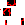
\includegraphics[width=0.25\textwidth]{Figures/fill_in_square.png}
	\caption{Terminal $A$-frozen parallel toppling odometer, $w_{\infty}$, on $\Z^2$ for initial conditions $w_0 = 1\{x \in A\}$ and $s_0' = 2+\Delta 1_A$. The set $A$ is denoted by red pixels and black pixels are sites which eventually topple.}
	\label{fig:fill_in}
\end{figure}


\begin{lemma}\label{lemma:local_convexity}
	Let $A := \{z^{(i)}\}$ be a finite path $z^{(i)} \sim z^{(i+1)}$.
	Let $w_t$ denote $A$-frozen parallel toppling with initial conditions 
	$w_0(x) = 1\{x \in A\}$ on the whole lattice (zero off $A$), $s_0' = \eta + \Delta w_0$. Then $w_t|_{\br(A)} = 1$ for every $t \geq |\br(A)|$.   
\end{lemma}
\begin{proof}
	By monotonicity of parallel toppling, we may take $\eta = (2 d - 2)$. Moreover, 
	it suffices to show that every site in $\br(A)$ eventually topples, as if no site topples at time $t$, then no site topples at time $(t+1)$.
	
	We say $A$ contains a $( \pm i, \pm j)$ turn if $z^{(m)} = z^{(m-1)} \pm  e_i$ and $z^{(m+1)} = z^{(m)} \pm e_j$
	for some $i \not = j$ where $z^{(m-1)} \sim z^{(m)} \sim z^{(m+1)}$ are in $A$.
	If $A$ does not contain a turn, then $\br(A) = A$. Hence, we may suppose it contains at least one turn.
	
	\subsubsection*{Case 1 - one-turn path}
	By shifting coordinates, we may suppose $A$ contains only a $(1,2)$ turn and that 
	\begin{equation}
	A = \{ 0, e_1, \ldots, k_1 e_1, k_1 e_1 + e_2, \ldots, k_1 e_1 + k_2 e_2 \}
	\end{equation}
	for $k_1 \geq k_2$.	We induct on $k_2$. If $k_2 = 1$, then after firing every site in $A$, 
	all sites in $A + e_2$ get one chip, while the corner site,
	$((k_1 - 1) e_1 + e_2)$ gets 2 chips. Since $\eta = (2 d- 2)$, that corner becomes unstable and fires, 
	causing all of its neighbors to the left, $((k_1 - 2) e_1 + e_2) \sim ((k_1 - 3) e_1 + e_2) \sim \cdots \sim e_2$ to fire. Continuing the induction shows that every site in $\br(A) = \{ x \in \Z^d : 0 \leq x \leq (k_1 e_1 + k_2 e_2)\}$ eventually fires. 
	
	\subsubsection*{Case 2 - cubic path} 
	We call $A$ a {\it cubic} path if, after an isometry, 
	\begin{equation}
	A = \{ 0, e_1, \ldots, k_1 e_1, k_1 e_1 + e_2, \ldots, \sum_{i=1}^d k_i e_i \}
	\end{equation}
	for $k_1 \geq \cdots \geq k_d \geq 0$. Let $d_0 := \max \{ i \leq d : k_i > 0 \}$. We induct on $d_0$, the base case $d_0 = 2$ established in Case 1. 
	For notational convenience, suppose the claim holds for $d_0 = (d-1)$ and we verify it for $d_0 = d$.
	
	
	Consider the $(d-1)$-turn subpaths, 
	\begin{equation}
	\begin{aligned}
	\mathcal{P}_1 &:= \{0, e_1, \ldots, \sum_{i=1}^{d-1} k_i e_i \} \\
	\mathcal{P}_2 &:= \{k_1 e_1, k_1 e_1 + e_2 , \ldots, \sum_{i=1}^{d} k_i e_i \}.
	\end{aligned}
	\end{equation}
	By the inductive hypothesis, after $\mathcal{P}_i$ fire,  
	both $(d-1)$-dimensional faces, 
	\begin{equation}
	\begin{aligned}
	\mathcal{F}_1 &:= \{x \in \Z^d : 0 \leq x \leq \sum_{i=1}^{d-1} k_i e_i \} \\
	\mathcal{F}_2 &:= \{x \in \Z^d : k_1 e_1 \leq x \leq \sum_{i=1}^{d} k_i e_i \}
	\end{aligned}
	\end{equation}
	fire. We then `fill in' the cube by identifying newly fired $(d-1)$-turn paths:
	\begin{equation}
	\begin{aligned}
	\mathcal{P}'_j := \{ & j  e_2, j e_2 + e_1, \ldots, j e_2 + k_1 e_1,  \\ 
	& j e_2 + k_1 e_1 + e_3, \ldots, j e_2 + k_1 e_1 + k_3 e_3, \\
	& \cdots \\
	&j e_2 + \sum_{i\not=2} k_i e_i \} 
	\end{aligned}
	\end{equation}
	which are in $\mathcal{F}_1 \cup \mathcal{F}_2$ for $j=0, \ldots, k_2$. By the inductive hypothesis, the firing of each $\mathcal{P}'_j$ makes every $(d-1)$-dimensional layer,
	\[
	\mathcal{L}_j := \{x \in \Z^d : j e_2 \leq x \leq j e_2 + \sum_{i\not=2} k_i e_i \},
	\]
	fire and $\br(A) = \cup_{j=0}^{k_2} \mathcal{L}_j$. 
	
	
	
	
	
	
	\subsubsection*{Case 3 - general path}
	
	It suffices to show that if there is a path of firings between any two distinct points $x,y$, 
	then $\br(\{x,y\})$ eventually fires. Before showing this, we suppose it were true and demonstrate sufficiency.
	Take $q \in \br(A)$ and observe by definition there are points $(z^{(1)}, Z^{(1)}), \ldots, (z^{(d)}, Z^{(d)})$ in $A$
	with $z_i^{(i)} \leq q_i \leq Z_i^{(i)}$.  Then,
	\[
	q^{(1)} := (q_1, \mathbf{q}_{d-1}') \in \br(\{z^{(1)}, Z^{(1)}\})
	\]
	for some $(d-1)$-vector $\mathbf{q}_{d-1}'$. Continue and let 
	\[
	q^{(2)} := \begin{cases}
	(q_1, q_2, \mathbf{q}_{d-2}'')  \in \br(\{q^{(1)}, z^{(2)}\}) &\mbox{ if $q^{(1)}_2 \geq q_2$}\\
	(q_1,q_2, \mathbf{q}_{d-2}''')  \in \br(\{q^{(1)}, Z^{(2)}\}) &\mbox{ otherwise }\\
	\end{cases}	
	\]
	for some $(d-2)$-vectors $\mathbf{q}_{d-2}'', \mathbf{q}_{d-2}'''$. After iterating, we find $q^{(d)} = q$, which shows that eventually $q$ will fire.
	
	
	Now fix two points $x,y \in A$ and decompose
	a path between them into a sequence of cubic paths
	\[
	\mathcal{P}^{(1)} := \bigcup_{i=1}^m \mathcal{P}^{(1)}_i, 
	\]
	where $\mathcal{P}^{(1)}_i := \{p_{i-1}, \ldots, p_i \}$ is cubic and $p_0 := x$ and $p_{m} := y$. (This can be done by, for example, 
	starting at x and exploring the path but cutting whenever the cubic condition is violated.) Case 2 shows that eventually every site in $\mathcal{A}^{(1)} := \bigcup_{i=1}^m \br(\mathcal{P}^{(1)}_i)$ will fire. 
	If $m = 1$, we are done, otherwise we construct a new cubic path from $p_0$ to $p_2$ 
	passing through $\mathcal{A}^{(1)}$. Once we have shown this, we
	iterate to conclude. 
	
	
	Suppose $p_0 = 0$, $p_{1} = \sum_{j=1}^d k_j e_j$, and 
	\[
	p_{2} = \sum_{j=1}^{d_1} (k_j-k_j') e_j  + \sum_{j=(d_1+1)}^{d_2} (k_j - k_j') e_j + \sum_{j=(d_2+1)}^{d} (k_j+k_j') e_j,
	\]
	for some $1 \leq d_1 \leq d_2 \leq d$ and $k_j,k_j' \geq 1$ where $(k_j - k_j') < 0$ for $j \leq d_1$ and $(k_j - k_j') \geq 0$
	for $(d_1 + 1) \leq j \leq d_2$. After this coordinate change, it suffices to exhibit a path from $p_0$ to $p_2$ with differences constrained to be $-e_j$ for $j = 1, \ldots, d_1$ and 
	$+e_j$ for $j = (d_1 + 1), \ldots, d$.
	
	There is a cubic path (only positive moves) from $p_0$ to
	\[
	w_1 := \sum_{j=(d_1+1)}^{d_2} (k_j - k_j') e_j + \sum_{j=(d_2+1)}^{d} (k_j) e_j
	\]
	contained within $\br(\{p_0, p_1\})$ as $p_0 = 0 \leq w_1 \leq p_1$. Then, since $w_1 \in \br(\{p_1,p_2\})$ there is a cubic path (only positive moves) from $w_1$ to 
	\[
	w_2 := w_1 + \sum_{j=(d_2+1)}^{d} k_j'e_j
	\]
	contained in $\br(\{p_1, p_2\})$ and similarly there is a cubic path (only negative moves) from $w_2$ to 
	\[
	p_2 = w_2  + \sum_{j=1}^{d_1} (k_j-k_j') e_j.
	\]
	Our new cubic path is the concatenation of these three paths: $p_0 \to w_1  \to w_2 \to p_2$. 
\end{proof}



\section{The last-wave}\label{sec:last_wave}
In this section we study a simplified parallel toppling procedure closely related to bootstrap percolation (see Section \ref{sec:criteria}
for an explicit connection, we do not utilize the coupling here). This simplified process has an inherent subadditive structure
which allows us to prove convergence using the subadditive ergodic theorem. In the next section we show that this process is a good approximation to an exploding sandpile. 


\subsection{\texorpdfstring{The $n$-wave process}{The n-wave process}} \label{subsec:n_wave}
Fix $n \geq 1$, $z \in \Z^d$, and consider the {\it $n$-wave} for $\eta$ starting at $z$,
\begin{equation} \label{eq:n_wave}
\begin{aligned}
u_0^{(n,z)} &:= n  \delta_z \\
u_{t+1}^{(n,z)}(x) &:= \lfloor \frac{ \sum_{y \sim x}  u_{t}^{(n,z)}(y) + \eta(x)}{2 d} \rfloor \mbox{ for $x \not= z$}.
\end{aligned}
\end{equation}
Note that there is intentionally no minimum in \eqref{eq:n_wave} with $u^{(n,z)}_t(x) + 1$
and it is possible that $u_{t+1}^{(n,z)}(x) > u_t^{(n,z)}(x) + 1$.
In particular, the $n$-wave started at $z$ dominates the $\{z\}$-frozen parallel toppling process defined in \eqref{eq:frozen_parallel_toppling} with the same initial conditions but may not coincide with it.

Overloading terminology, 
the $n$-wave is {\it stabilizable} if there is $T < \infty$
so that $u^{(n,z)}_{t} = u^{(n,z)}_{T}$ for all $t \geq T$. Let 
\begin{equation}
\hat{M}_{\eta}(z) := \min \{ n \geq 1 : \mbox{the $n$-wave for $\eta$ starting at $z$ is not stabilizable}\}.
\end{equation}


We write $u_t^{(z)} := u_t^{(\hat{M}_{\eta}(z),z)}$ for the $\hat{M}_{\eta}(z)$-wave starting at $z$ and call this the {\it last-wave}.  We also consider
the {\it penultimate-wave} starting at $z$ as the terminal odometer for the $(\hat{M}_{\eta}(z) - 1)$-wave, 
$\tilde{u}^{(z)}$, defined to be the zero function when $\hat{M}_{\eta}(z) = 1$. The set of sites touched by the penultimate wave is its {\it penultimate-cluster},
\begin{equation} \label{eq:penultimate_cluster}
\mathcal{P}(z) := \{z\} \cup \{ x \in \Z^d : \mbox{ there is $y \sim x$ with $\tilde{u}^{(z)}(y) > 0 $}\}
\end{equation}
(we included the point, $\{z\}$, as $\hat{M}_{\eta}(z)$ may be 1). When $z$ is the origin, we omit the superscripts. 


The {\it arrival time} for the last-wave starting at site $y$ to site $x$ is
\begin{equation} \label{eq:lastwave_fpp}
\hat{T}(y,x) := \min\{ t \geq 1 : u_{t}^{(y)}(x) > 0\}
\end{equation}
and the {\it penultimate-cluster arrival time} is 
\begin{equation} \label{eq:lastwave_modified_fpp}
\tilde{T}(y,x) := \min\{ t \geq 1 : u_{t}^{(y)}|_{\mathcal{P}(x)} > 0\}. 
\end{equation}
Note that the inequality in \eqref{eq:lastwave_modified_fpp} is strict --- $\tilde{T}(y,x)$ is the first time
the support of the last wave started at $y$ contains the entire penultimate wave of $x$, $\mathcal{P}(x)$. 
We write $\hat{T}(x) := \hat{T}(0,x)$ and $\tilde{T}(x) := \tilde{T}(0,x)$.
(The choice of the same letter $T$ for all arrival times is intentional --- we will see they are asymptotically close.)

\subsection{Basic properties of the last-wave} \label{sec:last_wave_basic_properties}
We derive some basic properties of the last-wave. Throughout this section and the next, let $\eta$ be drawn from the event of probability 1 in Proposition~\ref{prop:renormalization_properties} and let $k$ be the (deterministic but large) side length of a good cube.

For the wave in~\eqref{eq:n_wave}, the value at its starting site is frozen: $u_t^{(m,z)}(z)=m$ for every $t\geq0$. The parameter $m\in\N$ is a prescribed toppling count, not a number of added chips or a time horizon. Here the support of a wave means $\{x:\text{there exists }t\geq0\text{ with }u_t^{(m,z)}(x)>0\}$. Write $\Lambda_n=[-n,n]^d\cap\Z^d$ for the cube of radius $n$. The quantitative estimate below uses a lower bound on the radius of the toppled cube from Fey, den Boer and Redig~\cite{fey2008limiting} and an upper bound on the toppled set from Fey, Levine and Peres~\cite{fey2010growth}.

\begin{lemma}\label{lemma:square_lower_bound}
For each integer $d\geq2$ there is a deterministic constant $C_d>0$ with the following property. Let $\eta:\Z^d\to\Z$ satisfy $2d-2\leq\eta(x)\leq2d-1$ at every site. For every integer $n\geq1$ and every integer $m\geq1$ satisfying
\begin{equation*}
 m\geq
 \begin{cases}
 \lceil C_2 n^2\log(n+1)\rceil,&d=2,\\
 \lceil C_d n^d\rceil,&d\geq3,
 \end{cases}\,,
\end{equation*}
there exists a finite integer $T$ such that $u_t^{(m,0)}(x)>0$ for every $t\geq T$ and every $x\in\Lambda_n$. In particular the support of this wave contains $\Lambda_n$.
\end{lemma}

\begin{proof}
Set $h=2d-2$. Let $\Delta$ be the unnormalized Laplacian, $\Delta f(x)=\sum_{y\sim x}f(y)-2df(x)$. For $N\geq2$, let $v_N$ be the terminal ordinary toppling odometer for $h+N\delta_0$, and let $s_N=h+N\delta_0+\Delta v_N$. Throughout this proof $N$ counts extra chips and $m$ counts frozen origin topplings. Ordinary legal toppling preserves nonnegative heights, so $0\leq s_N\leq2d-1$.

\emph{Step 1.} We show that $\Lambda_n\subseteq\operatorname{supp}v_N\subseteq\mathcal D$ for the choice of $N$ and $\mathcal D$ made below, using two cited radius bounds.

Theorem 4.1 of Fey, den Boer and Redig~\cite{fey2008limiting} gives finite stabilization and a cubical toppled set $\operatorname{supp}v_N=\Lambda_{r_N}$, with
\begin{equation*}
 r_N\geq\frac{N^{1/d}-3}{2}\,.
\end{equation*}
Their model parametrizes the total origin height, which is $N+h$ here, so their lower bound with $N+h$ implies the bound with $N$. Equivalently, once the cubical shape is known, chip conservation gives $N=\sum_x(s_N(x)-h)\leq|\Lambda_{r_N+1}|=(2r_N+3)^d$, because all height changes lie in $\Lambda_{r_N+1}$, each increase is at most one, and the sum of the finitely supported Laplacian is zero.

Theorem 1.1 of Fey, Levine and Peres~\cite{fey2010growth}, applied at $h=2d-2$ and $\epsilon=1$, gives
\begin{equation*}
 \operatorname{supp}v_N\subseteq\Lambda_{A_dN^{1/d}},\qquad
 A_d=(d+1)\omega_d^{-1/d}\,,
\end{equation*}
for all sufficiently large $N$, where $\omega_d$ is the volume of the Euclidean unit ball. Its hypothesis $d\leq h\leq2d-2$ holds for every $d\geq2$ considered here. The bound concerns toppled sites, not the particle cluster with its extra boundary. Choose an integer $N_0(d)\geq2$ so the bound holds for every $N\geq N_0(d)$, and in the remainder take
\begin{equation*}
 N=(2n+3)^d+N_0(d),\qquad L=\lceil A_dN^{1/d}\rceil,\qquad \mathcal D=\Lambda_L\,.
\end{equation*}
Thus $\Lambda_n\subseteq\operatorname{supp}v_N\subseteq\mathcal D$, including for $n=1$.

\emph{Step 2.} We show that the walk killed on leaving $\mathcal D$ has a Green function $G_{\mathcal D}$ with $G_{\mathcal D}(0,0)$ and $\sum_{y\in\mathcal D}G_{\mathcal D}(0,y)$ bounded in terms of $L$.

Let $X_t$ be the continuous-time simple random walk with total jump rate one, each jump uniformly chosen among the $2d$ neighbors. Its generator is $P-I=\Delta/(2d)$. Put $\tau=\inf\{t\geq0:X_t\notin\mathcal D\}$ and
\begin{equation*}
 p_{\mathcal D}(t,x,y)=\mathbf P_x(X_t=y,\ t<\tau),\qquad
 G_{\mathcal D}(x,y)=\int_0^\infty p_{\mathcal D}(t,x,y)\,dt\,.
\end{equation*}
The holding times have mean one and are independent of the embedded walk, so $G_{\mathcal D}$ also equals the usual discrete-time expected number of visits before exit.

For each starting site $x\in\mathcal D$, the process $|X_t|_2^2-t$ is a martingale: averaging one jump increases squared norm by one. Bounded stopping at $t\wedge\tau$ gives
\begin{equation*}
 \mathbf E_x(t\wedge\tau)
 =\mathbf E_x|X_{t\wedge\tau}|_2^2-|x|_2^2
 \leq d(L+1)^2=:b\,.
\end{equation*}
The stopped walk lies in $\Lambda_{L+1}$, including the exit point. Monotone convergence proves $\mathbf E_x\tau\leq b$ and almost-sure exit, uniformly in $x$. Markov's inequality gives $\mathbf P_x(\tau>2b)\leq1/2$. The Markov property, successively at the deterministic times $2b,4b,\ldots$, therefore gives
\begin{equation*}
 \sup_{x\in\mathcal D}\mathbf P_x(\tau>t)\leq2^{-\lfloor t/(2b)\rfloor}\,.
\end{equation*}
This also proves integrability of every entry of the killed semigroup.

The coordinates of $X_t$ are independent symmetric continuous-time one-dimensional walks of rate $1/d$, by independent Poisson splitting of the jump directions. Fourier inversion of their integer-valued distributions gives, for the unrestricted transition probability $q(t,0,z)$,
\begin{equation*}
 |q(t,0,z)|\leq
 \left(\frac1{2\pi}\int_{-\pi}^{\pi}
 e^{-(t/d)(1-\cos\theta)}d\theta\right)^d
 \leq\min\{1,(d\pi/(8t))^{d/2}\}
 \leq K_d(1+t)^{-d/2}\,.
\end{equation*}
For completeness, the one-dimensional characteristic function is $\exp[(t/d)(\cos\theta-1)]$, obtained by summing its Poisson number of independent symmetric jumps. Fourier inversion follows by integrating $e^{i\theta(k-z)}$, whose integral is $2\pi$ if $k=z$ and zero otherwise; absolute summability permits exchanging the probability sum and integral. For the second inequality use $1-\cos\theta\geq2\theta^2/\pi^2$ on $[-\pi,\pi]$ and enlarge the Gaussian integral to the real line. The last inequality holds with, for example, $K_d=(1+\sqrt{d\pi/8})^d$.

The killed transition matrix is symmetric. Its semigroup identity and $0\leq p_{\mathcal D}\leq q$ now imply
\begin{equation*}
 \begin{aligned}
 p_{\mathcal D}(t,0,0)&=\sum_{y\in\mathcal D}p_{\mathcal D}(t/2,0,y)^2\\
 &\leq K'_d(1+t)^{-d/2}\sum_{y\in\mathcal D}p_{\mathcal D}(t/2,0,y)\\
 &\leq K'_d(1+t)^{-d/2}2^{-\lfloor t/(4b)\rfloor}\,.
 \end{aligned}
\end{equation*}
For $d=2$, integrate over $[0,4b]$ to get at most $K'_2\log(1+4b)$. On each interval $[4bk,4b(k+1)]$, $k\geq1$, the integral is at most $K'_2 2^{-k}/k$. For $d\geq3$, simply discard the survival factor and use $\int_0^\infty(1+t)^{-d/2}dt=2/(d-2)$. Consequently
\begin{equation*}
 G_{\mathcal D}(0,0)\leq
 \begin{cases}
 C\log(L+2),&d=2,\\
 C_d,&d\geq3,
 \end{cases}
 \qquad \sum_{y\in\mathcal D}G_{\mathcal D}(0,y)=\mathbf E_0\tau\leq d(L+1)^2\,.
\end{equation*}

\emph{Step 3.} We show that $v_N(0)\leq CN\log(N+1)$ for $d=2$ and $v_N(0)\leq C_dN$ for $d\geq3$, using the Green function of Step 2.

Let $P_{\mathcal D}$ be the killed discrete transition matrix on $\mathcal D$, with zero extension outside. Then $p_{\mathcal D}(t)=e^{-t(I-P_{\mathcal D})}$. Its integrable entries and the survival bound show that $p_{\mathcal D}(t)\to0$; integrating its derivative on $[0,R]$ and passing to the limit gives $(I-P_{\mathcal D})G_{\mathcal D}=G_{\mathcal D}(I-P_{\mathcal D})=I$. Thus $I-P_{\mathcal D}$ is invertible, with inverse $G_{\mathcal D}$. Since $v_N=0$ off $\mathcal D$, its conservation equation is exactly
\begin{equation*}
 (I-P_{\mathcal D})v_N=\frac{N\delta_0-(s_N-h)}{2d}\,.
\end{equation*}
Multiplication by this inverse gives
\begin{equation*}
 v_N(0)=\frac{N}{2d}G_{\mathcal D}(0,0)
       -\frac1{2d}\sum_{y\in\mathcal D}G_{\mathcal D}(0,y)(s_N(y)-h)\,.
\end{equation*}
The sign and normalization follow from $\Delta=2d(P-I)$. Since $s_N-h\geq-h$, positivity of $G_{\mathcal D}$ gives
\begin{equation*}
 v_N(0)\leq\frac{N}{2d}G_{\mathcal D}(0,0)+\frac{h}{2d}\mathbf E_0\tau
 \leq\begin{cases}
 C N\log(N+1),&d=2,\\
 C_d N,&d\geq3,
 \end{cases}\,.
\end{equation*}
Indeed, $L+1\leq A_dN^{1/d}+2$, and $N^{2/d}\leq N$ for $N\geq1$. Furthermore $N\leq(5^d+N_0(d))n^d$ for $n\geq1$, and in dimension two $\log(N+1)\leq C_2\log(n+1)$. Enlarge the deterministic constants so the lemma's lower bound on $m$ implies $m\geq v_N(0)$.

\emph{Step 4.} We show that $u_t^{(m,0)}(x)>0$ for every $x\in\Lambda_n$ and every $t\geq T$, for a finite time $T$.

Let $a_t$ be the ordinary parallel odometer for $h+N\delta_0$, starting from zero. At every time its height is nonnegative: a toppled site loses $2d$ only when it has at least $2d$, and all incoming chips are nonnegative. Away from zero the exact ordinary recurrence is therefore
\begin{equation*}
 a_{t+1}(x)=\min\left\{a_t(x)+1,
 \left\lfloor\frac{\sum_{y\sim x}a_t(y)+h}{2d}\right\rfloor\right\}\,.
\end{equation*}
To verify this, the numerator is $2da_t(x)+s_t(x)$. For $0\leq s_t(x)<2d$ its floor is $a_t(x)$; for $s_t(x)\geq2d$ the minimum is $a_t(x)+1$. At zero, $a_t(0)\leq v_N(0)\leq m$. Inductively $a_t\leq u_t^{(m,0)}$: the base case follows from $a_0=0\leq m\delta_0$, the origin is frozen at $m$, and away from zero use this recurrence, the monotone neighbor sum and floor, and $h\leq\eta$. Ordinary stabilization occurs at a finite time $T$, so $u_T^{(m,0)}\geq v_N>0$ on $\Lambda_n$.

Finally, for every background with $0\leq\eta\leq2d-1$, the wave is nonnegative, nondecreasing in time, and at most $m$. Nonnegativity and the upper bound follow by induction in its floor recurrence. For time monotonicity first $u_1\geq u_0$ (with equality at zero), and then use monotonicity of the update map. Hence positivity on $\Lambda_n$ persists for every $t\geq T$.
\end{proof}

The constant $C_d$ does not depend on the background, and the lemma gives no bound on $T$.

For a background bounded below only by an integer $\eta_{\min}$, as in Section~\ref{sec:generalization}, the wave~\eqref{eq:n_wave} need not be nonnegative: if $x\neq0$ is not adjacent to the origin and $\eta(x)<0$, then $u_1^{(m,0)}(x)=\lfloor\eta(x)/(2d)\rfloor<0$. Under Hypothesis~\ref{hyp:path_filling}, Step~1 of the proof of Proposition~\ref{prop:convergence_of_the_generalized_last_wave} shows that $\eta\geq0$ almost surely, so $0\leq\eta\leq2d-1$ holds almost surely there, and the exponential path argument for nonnegative backgrounds in Step~4 of that proof gives only a qualitative seeding, with no polynomial rate.

\begin{remark}[Sharp planar obstruction]\label{rem:sharp_planar_obstruction}
On homogeneous height $2$ in dimension two, the least integer order $M_2(n)$ whose wave covers $\Lambda_n$ satisfies
\begin{equation*}
 c n^2\log(n+1)\leq M_2(n)\leq C n^2\log(n+1)\,,
\end{equation*}
for every $n\geq1$.
We prove the lower bound first; the upper bound is Lemma~\ref{lemma:square_lower_bound}.
For sufficiently large $N$, the radius bound of Fey, Levine and Peres~\cite{fey2010growth} permits $L=\lceil2\sqrt N\rceil$ and $\operatorname{supp}v_N\subseteq\Lambda_L$.
The Green identity above and $s_N-2\leq1$ give
\begin{equation*}
 v_N(0)\geq\frac N4G_{\Lambda_L}(0,0)-\frac14\mathbf E_0\tau\,.
\end{equation*}
For the embedded discrete walk $S_j$, exit from $\Lambda_L$ is impossible by time $2j\leq L$. The increments of $S^1+S^2$ and $S^1-S^2$ are independent symmetric signs, so $\mathbf P(S_{2j}=0)=[\binom{2j}j/4^j]^2\geq1/(4j)$ for $j\geq1$. The binomial inequality follows by induction: its value at $j=1$ is $1/2$, and the ratio of successive values is $(2j+1)/(2j+2)\geq\sqrt{j/(j+1)}$. Therefore
\begin{equation*}
 v_N(0)\geq\frac N4+\frac N{16}H_{\lfloor L/2\rfloor}
                   -\frac{(L+1)^2}{2},\qquad H_k=\sum_{j=1}^k\frac1j\,.
\end{equation*}
Taking $N=\lfloor n^2/16\rfloor$ gives $L<n$ and $v_N(0)\geq c n^2\log(n+1)$ for all sufficiently large $n$.
The comparison in the opposite direction is proved by a further induction: if an integer-valued $w\geq0$ satisfies $w(0)\geq m$ and $2+\Delta w\leq3$ off zero, then $u_t^{(m,0)}\leq w$ at every time. At zero this is the frozen inequality; away from zero use $\sum w+2\leq4w(x)+3$ and integrality to bound the floor by $w(x)$. Applying this to $w=v_N$ shows that every $m\leq v_N(0)$ misses $\Lambda_n$. For the finitely many remaining $n$, $M_2(n)\geq1$, so reducing $c>0$ extends the lower bound to all $n\geq1$; Lemma~\ref{lemma:square_lower_bound} supplies the upper bound at every scale. No matching lower bound is claimed for arbitrary backgrounds: on homogeneous height $3$ a $1$-wave propagates to every site by induction on lattice distance.
\end{remark}





\begin{lemma} \label{lemma:finite_exploding}
	The last-wave is well-defined, $\hat{M}_{\eta}(0) < \infty$.
\end{lemma}
\begin{proof}
	By Lemma \ref{lemma:square_lower_bound}
	and Proposition \ref{prop:renormalization_properties}, if the origin is fired a sufficient number of times, the support of the odometer contains a good cube, $Q_k \subset \mathcal{C}_{\infty}$.
\end{proof}



\begin{lemma} \label{lemma:last_wave_bound}
	The last wave started at $z$ is bounded by one outside the interior of the penultimate-cluster of $z$. Moreover, for all $t \geq 1$ and $x,z \in \Z^d$, 
	\[
	u_t^{(z)}(x) \leq (1 + \tilde{u}^{(z)}(x)).
	\]
\end{lemma}

\begin{proof}
	To reduce clutter, we take $z = 0$. We prove this by induction on $t$. 
	The base case $t=0$ follows by definition. For all $t \geq 1$, the definition also ensures it holds at the origin.
	So, we may take $x \not = 0$ and check:
	\begin{align*}
	u_{t+1}(x) &= \lfloor \frac{ \sum_{y \sim x}  u_{t}(y) + \eta(x)}{2 d} \rfloor \\
	&\leq \lfloor \frac{ \sum_{y \sim x} (1 + \tilde{u}(y)) + \eta(x)}{2 d} \rfloor \\
	&= 1 + \tilde{u}(x) + \lfloor \frac{ \sum_{y \sim x} (\tilde{u}(y)-\tilde{u}(x)) + \eta(x)}{2 d} \rfloor \\
	&= 1 + \tilde{u}(x)
	\end{align*}
	as $\Delta \tilde{u}(x) + \eta(x) \leq (2 d- 1)$ for $x \not = 0$. 
	
	
	
	
	
	
	
\end{proof}




\begin{lemma} \label{lemma:approx_subadditivity}
	The penultimate-cluster arrival times are subadditive: for all $a,b,z \in \Z^d$, 
	\[
	\tilde{T}(a,z) \leq \tilde{T}(a,b) + \tilde{T}(b, z).
	\]	
\end{lemma}
\begin{proof}
	Suppose $\mathcal{P}(z) \not \subseteq \mathcal{P}(b)$, otherwise the claim is immediate.
	It suffices to check  
	\begin{equation}
	w_t(x)  := u_{\tilde{T}(a,b)+t}^{(a)}(x) \geq u_{t}^{(b)}(x) \qquad \mbox{for all $t \geq 1$ and $x \in \mathcal{P}(b)^c$},
	\end{equation}
	which we do by induction. 
	By Lemma \ref{lemma:last_wave_bound}, $u_t^{(b)}(x) \leq 1$ if $\tilde{u}^{(b)}(x) = 0$. 
	Also, by definition of the penultimate-cluster, we have that $\tilde u^{(b)}$  is zero 
	on $\partial^{\circ} \mathcal{P}(b)$.
	Hence, for all $t \geq 1$ and $x \in \partial^{\circ} \mathcal{P}(b)$,  $u_t^{(b)}(x) \leq 1 \leq w_t(x)$.
	Using this and the inductive hypothesis, if $x \in \mathcal{P}(b)^c \cap \{a\}^c$, 
	\begin{align*}
	w_{t+1}(x) &= \lfloor \frac{ \sum_{y \sim x} w_t(y) + \eta(x) }{ 2d} \rfloor \\
	&\geq  \lfloor \frac{ \sum_{y \sim x} u_{t}^{(b)}(y) + \eta(x) }{ 2d} \rfloor \\
	&=  u_{t+1}^{(b)}(x).
	\end{align*}
	If $x \in \mathcal{P}(b)^c \cap \{a\}$, then $w_t(x) \geq 1 \geq u_t^{(b)}(x)$ as $\hat{M}_{\eta}(a) \geq 1$. 
	
	
	
	
\end{proof}



\begin{lemma} \label{lemma:last_penultimate_cluster}
	There is a constant $\gamma > 0$ so that for all $n$ sufficiently large 
	and $|x| \leq n$, 
	\[
	\mathcal{P}(x) \subset x + [-(\log n)^{\gamma}, (\log n)^{\gamma}]^d.
	\]	
\end{lemma}
\begin{proof}
	By Lemma \ref{lemma:local_convexity}, $1\{ \tilde{u}^{(x)} > 0 \}$ is a rectangle,
	therefore it suffices to bound the maximal side length. By Proposition \ref{prop:renormalization_properties},
	for all $n$ sufficiently large, if any side length of the rectangle exceeds  $(2 k \log n)^{5/2}$ then it
	must overlap a good cube, contradicting stability. 
\end{proof}


\begin{lemma} \label{lemma:penultimate_upper_bound}
	There are constants $\gamma$ and $C$ so that on an event of probability 1, for all $n$ sufficiently large and $|x| \leq n$, 
	\[
	\hat{T}(x) \leq  C |x| +  (\log n)^{\gamma} .
	\]
\end{lemma}
\begin{proof}
	Let $x \in \Z^d$ be given. Since the sandpile is exploding, at some constant time $C_\eta$
	the support of the odometer will overlap the infinite cluster at a good cube near the origin, $Q_k(z)$ for some $z \in \Z^d$. Once this occurs the arrival time to any site is at most a constant times the chemical distance in the infinite cluster. Let $Q_k(y)$ for $y \in \Z^d$ be one of the nearest cubes in $\mathcal{C}_{\infty}$ to $x$.  There are now two cases to consider.
	
	
	If $|z-y| < (\log n)^2$, then we may choose nearby points $M_{i} \in \mathcal{C}_{\infty}$ so that $(\log n)^{c} \leq d(z,M_i) \leq (\log n)^C$ and $x,y \in \br(\{M_i\})$. 
	If $|z-y| \geq (\log n)^2$, then by the chemical distance bound and the definition of $\mathcal{C}_{\infty}$, 
	within at most $C |z-y| \leq C(|z| + |y|)$ steps, $Q_k(y)$ will topple. 
	Once this happens, $\mathcal{P}(x)$ is surrounded in at most $(\log n)^C$ more steps and $\mathcal{P}(x)$ will fire in at most $|\mathcal{P}(x)|$ additional steps.
	
\end{proof}





\subsection{Convergence of the last-wave}
We show that the arrival time for the last-wave converges under rescaling. 

\begin{lemma} \label{lemma:last_penultimate_close}
	There exists a constant $\gamma > 0$ so that on an event of probability 1, for all $n$ sufficiently large and $|x| \leq n$,
	\[
	\hat{T}(x) \leq \tilde{T}(x) \leq \hat{T}(x) + (\log n)^{\gamma}.
	\]
\end{lemma}
\begin{proof}
	The first inequality is immediate.  For the second inequality, let $C$ and $n_0$ be as in Proposition \ref{prop:renormalization_properties}.
	Take $n \geq n_0$ and suppose $v_t(x) > 0$ for $\min(t, |x|) > C$ and $|x| \leq n$.  We must show that there is a nearby good cube $Q_k(y) \subset \mathcal{C}_{\infty}$
	which has already fired. Once we have shown this, the same argument as in Lemma \ref{lemma:penultimate_upper_bound}
	allows us to conclude. 	This is, however, a consequence of Lemma \ref{lemma:local_convexity} and Proposition \ref{prop:renormalization_properties}. Any path of topplings of length at least $( 2k \log n)^{5/2}$ must overlap a good cube. 
\end{proof}


\begin{prop} \label{prop:convergence_of_the_last_wave}
	On an event of probability 1, the rescaled last-wave arrival times 
	\[
	n^{-1} \hat{T}_{\eta}([n x])
	\] 
	converge locally uniformly to $\mathcal{N}_{p}$, a continuous, convex, one-homogeneous function on $\R^d$. 
\end{prop}
\begin{proof}
	In light of Lemma~\ref{lemma:last_penultimate_close} it suffices to prove the result for $\tilde{T}$. On an event of probability 1, for all large $n$ and $x,x'\in[-n,n]^d$, Lemmas~\ref{lemma:penultimate_upper_bound} and~\ref{lemma:last_penultimate_close} give $\tilde{T}(x)\leq C|x|+(\log n)^{\gamma}$, and $\tilde{T}(x')\leq\tilde{T}(x)+C|x-x'|+(\log n)^{\gamma}$.
	For the second bound, at time $\hat{T}(x)$ the support of the last wave contains a path of distinct points from the origin to $x$. Lemma~\ref{lemma:local_convexity} fills the bounding rectangle of the last $(\log n)^{\gamma'}$ points of this path, where $\gamma'$ is the constant of Lemma~\ref{lemma:last_penultimate_cluster}. This rectangle contains a line of a cube of $\mathcal{C}_{\infty}$ by Proposition~\ref{prop:renormalization_properties}, and the argument of Lemma~\ref{lemma:penultimate_upper_bound} then reaches $\mathcal{P}(x')$.
	Fix $y\in\Z^d\setminus\{0\}$. Choose $C'>C|y|$ and $K$ so large that $A=\{\tilde{T}(0,ny)\leq C'n+K \text{ for every } n\geq1\}$ has $\mathbf{P}(A)>0$. This is possible because $\tilde{T}(0,ny)\leq C|y|n+(\log(n|y|))^{\gamma}$ for all large $n$ on an event of probability 1, and $(\log(n|y|))^{\gamma}=o(n)$. Let $\sigma_y$ be the translation of the background by $y$, $(\sigma_y\eta)(x)=\eta(x+y)$, so that $\tilde{T}(y,ny)=\tilde{T}(0,(n-1)y)\circ\sigma_y$. The translation $\sigma_y$ is mixing, hence ergodic, and the first-return map to $A$ preserves the restriction of the probability measure to $A$ and is ergodic. With $r_j$ the successive return times and $S_j=r_1+\dots+r_j$, the induced cocycle $G_j=\tilde{T}(0,S_jy)$ is subadditive by Lemma~\ref{lemma:approx_subadditivity}, and $G_1\leq C'r_1+K$ on $A$. The return time $r_1$ is integrable on $A$ by Kac's lemma, so the subadditive ergodic theorem applies to $G_j$ with no integrability bound on $\tilde{T}$ itself.
	The second bound passes from the return times to all $n$: for $S_j\leq n<S_{j+1}$ it gives $|\tilde{T}(0,ny)-G_j|\leq C r_{j+1}+(\log n)^{\gamma}$, and $r_{j+1}/j\to0$ almost surely by Birkhoff's theorem applied to the integrable $r_1$. Hence on $A$ the limit inferior and superior of $n^{-1}\tilde{T}(0,ny)$ are those of $G_j/S_j$, which converge because $G_j/j$ converges by Kingman's theorem and $S_j/j$ converges by Birkhoff's theorem.
	The limits inferior and superior of $n^{-1}\tilde{T}(0,ny)$ are invariant under $\sigma_y$: by Lemma~\ref{lemma:approx_subadditivity}, $\tilde{T}(0,ny)$ and $\tilde{T}(y,ny)=\tilde{T}(0,(n-1)y)\circ\sigma_y$ differ by at most the finite quantity $\tilde{T}(0,y)+\tilde{T}(y,0)$. By ergodicity they are almost surely constant, and they agree on $A$, so the limit exists almost surely. The second bound replaces continuity: it supplies the comparison needed to pass from integer directions to all $x$, giving locally uniform convergence, and the properties of $\mathcal{N}_p$ are immediate from the scaling and microscopic subadditivity.
\end{proof}

\begin{remark}
	Convergence of the last wave may be viewed as a sort of bootstrap percolation shape theorem. 
	Sites are initially randomly assigned two thresholds, 1 or 2. A site with threshold $l$
	becomes infected when at least $l$ of its neighbors are infected. Infected sites remain infected. 
	The above shows that if you start off with a large enough cluster of infected sites at the origin, every site will eventually become 
	infected and the speed at which the infection spreads converges. 
	
	For more on the relationship between sandpiles and bootstrap percolation, see Section \ref{sec:criteria} below. 
	Similar shape theorems include \cite{garet2012asymptotic, kesten2008shape,alves2002shape, cox1981some} and 
	especially \cite{willson1978convergence, gravner1993threshold,fey2010limiting}.
\end{remark}




\section{Proof of Theorem \ref{theorem:convergence_of_time_constant}} \label{sec:proof_of_theorem}
Let $\eta$ be drawn from the event of full probability in Proposition \ref{prop:convergence_of_the_last_wave}.
It suffices to show that the last-wave is a good approximation of the original process. 


\begin{prop} \label{prop:approximate_subadditive}
	On an event of probability 1, there are constants $C_1(\eta), C_2(\eta)$
	so that for all $x \in \Z^d$, 
	\begin{equation} \label{eq:ineq1}
	T(x) \leq \hat{T}(x) + C_1(\eta)
	\end{equation}
	and
	\begin{equation} \label{eq:ineq2}
	\hat{T}(x) \leq T(x) + C_2(\eta),
	\end{equation}
	where the last-wave arrival time $\hat{T}$ is defined in \eqref{eq:lastwave_fpp}  
	and $T(x) := \min \{ t \geq 0 : v_t(x) > 0 \}$. 
\end{prop}
\begin{proof}
	
	Recall that $v_t$ is the parallel toppling odometer for $\eta + M_{\eta}  \delta_0$ and recall the last-wave odometer $u_t$ from Section \ref{subsec:n_wave}.
	
	We first check \eqref{eq:ineq1}. 
	Let $u'_t$ be the $\mathcal{P}(0)$-frozen parallel toppling odometer with initial conditions $u'_0(x) = 1\{x \in \mathcal{P}(0)\}$ and
	$s_0' = \eta + \Delta u'_0$ 
	where $\mathcal{P}(0)$ is the penultimate-cluster for $0$ defined in \eqref{eq:penultimate_cluster}.
	By Lemma \ref{lemma:last_wave_bound}, for all $t \geq 0$, $u_{t}$ is at most 1 on the inner boundary of the penultimate-cluster, $\partial^{\circ} \mathcal{P}(0)$.  
	Hence, as $\eta \leq (2 d -1)$, 
	by \eqref{eq:frozen_parallel_toppling_recurse} and the definition of the last-wave we have $u'_t |_{\mathcal{P}(0)^c} \geq u_t |_{\mathcal{P}(0)^c}$ for all $t \geq 0$. Also, since $\eta + M_{\eta}  \delta_0$ is not stabilizable, for some $t_0 \geq C_{\eta}$, $v_{t_0} |_{\mathcal{P}(0)} \geq u'_{0} |_{\mathcal{P}(0)}$. 
	Hence by \eqref{eq:odometer_wave_comp}, $v_{t + t_0} |_{\mathcal{P}(0)^c} \geq u'_t |_{\mathcal{P}(0)^c} \geq u_t |_{\mathcal{P}(0)^c}$ for all $t \geq 0$, 
	completing the check of \eqref{eq:ineq1}
	
	
	%	We first observe that \eqref{eq:ineq1} follows immediately from \eqref{eq:odometer_wave_comp}:
	%	since $\hat{M}_{\eta}(0) < \infty$, and $\eta + M_{\eta}  \delta_0$ is not stabilizable, for $t \geq C_{\eta}$,
	%	$v_{t}(0) \geq \hat{M}_{\eta}(0) = u_0(0)$.  
	%	
	We now verify \eqref{eq:ineq2}. We first consider the special case where only
	one firing at the origin is needed to have an infinite last-wave. 
	
	\subsection*{Step 1: Special case,  \texorpdfstring{$\hat{M}_{\eta}(0) = 1$}{One firing} }
	Denote the reachable sets up to time $t$ for the last wave and exploding sandpile as 
	\begin{equation} \label{eq:reachablesets_definition}
	\begin{aligned}
	\mathcal{R}_t &:= \{ x \in \Z^d : v_t(x) > 0 \} \\
	\hat{\mathcal{R}}_t &:= \{ x \in \Z^d : u_t(x) > 0 \}.
	\end{aligned}
	\end{equation}
	Note, by minimality, if $\hat{M}_{\eta}(0) = 1$, then $\eta(0) + M_{\eta}(0) = 2 d$. 
	This together with $\eta \geq (2 d- 2)$, implies a strong regularity. 
	Specifically, we show by induction that for all $t \geq 0$,
	\begin{equation} \label{eq:induction1}
	\mathcal{R}_t \subseteq \hat{\mathcal{R}}_t 
	\end{equation}
	and 
	\begin{equation} \label{eq:induction2}
	\begin{aligned}
	|v_t(x \pm e_i \pm e_j) - v_t(x)| &\leq 1  \qquad \mbox{for all $x \in \Z^d$ and $e_i \not = e_j$} \\
	|v_t(x \pm e_i) - v_t(x)| &\leq 1   \qquad \mbox{for all $x \in \Z^d$ and $e_i$}
	\end{aligned}
	\end{equation}
	and 
	\begin{equation} \label{eq:induction3}
	v_t(0) \geq \max_{x \in \Z^d} v_t(x).
	\end{equation}
	The base case $t = 0$ is immediate, so suppose \eqref{eq:induction1}, \eqref{eq:induction2}, and \eqref{eq:induction3}
	hold at $t \geq 0$ and we check $(t+1)$.  
	\subsubsection*{Inductive step for \eqref{eq:induction3}}
	\eqref{eq:parallel_toppling_recursion} and \eqref{eq:induction3} at time $t$ imply
	if $x \not = 0$, 
	\begin{align*}
	v_{t+1}(x) &\leq \lfloor \frac{2 d  v_t(0) + \eta(x) }{2 d} \rfloor \\
	&= v_t(0) + \lfloor \frac{\eta(x)}{2 d} \rfloor \\
	&= v_t(0) \\
	&\leq v_{t+1}(0),
	\end{align*}
	as $\eta \leq (2 d - 1)$. 
	
	\subsubsection*{Inductive step for \eqref{eq:induction2}}
	We first check the origin. By \eqref{eq:induction3}, if $v_t(y) = v_t(0)-1$
	for some $y \sim 0$, then $\Delta v_t(0) + 2 d \leq (2 d -1)$. Otherwise, 
	suppose $v_t(e_i + e_j) = v_t(0) - 1$ for some $e_i \not = e_j$ and the origin is unstable at time $t$. Then,
	$v_t(e_i) = v_t(0)$ and $v_t(e_j) = v_t(0)$. This implies, by \eqref{eq:induction2} applied to $e_i$ and $e_j$, that all other neighbors $y \sim (e_i + e_j)$ have a lower bound, $v_t(y) \geq v_t(0) - 1$. 
	Hence, $\Delta v_t(e_i + e_j) \geq 2$, which implies that $(e_i+e_j)$ is unstable at time $t$
	using $\eta \geq (2 d - 2)$. 
	
	Now, take $x \not = 0$ and suppose for sake of contradiction 
	\begin{equation} \label{eq:unstable}
	\Delta v_t(x) + \eta(x) \geq 2 d
	\end{equation}
	but for some adjacent neighbor $(x + e_j)$,  
	\begin{equation} \label{eq:stable_neighbor1}
	v_t(x+e_j) = v_t(x) - 1 \qquad \mbox{and} \qquad  \Delta v_t(x+e_j) + \eta(x+e_j) \leq 2 d -1.
	\end{equation}
	At least two other adjacent neighbors, $y' \sim x$ must satisfy $v_t(y') = v_t(x) + 1$.
	Indeed, otherwise by \eqref{eq:stable_neighbor1} and \eqref{eq:induction2},	 $\Delta v_t(x) \leq 0$, violating
	our assumption \eqref{eq:unstable}. However, one of those neighbors must be 
	$y' = x \pm e_i$ for some $e_i \not= e_j$. This contradicts
	\eqref{eq:induction2} at time $t$ since 
	\[
	v_t(x + e_i) = v_t(x + e_i + (-e_i + e_j)) + 2.
	\]
	
	Next, take a diagonal neighbor,  $(x + e_i + e_j)$ for $i \not = j$, and suppose for sake of contradiction \eqref{eq:unstable}
	but
	\begin{equation} \label{eq:stable_neighbor2}
	v_t(x+e_i+e_j) = v_t(x) - 1 \qquad \mbox{and} \qquad  \Delta v_t(x+e_i+e_j) + \eta(x+e_i+e_j) \leq (2 d -1).
	\end{equation}
	By \eqref{eq:unstable} there must be at least one adjacent neighbor $y \sim x$ with $v_t(y) = v_t(x) + 1$.
	This neighbor cannot be $(x+e_i)$ or $(x+e_j)$ as it would contradict \eqref{eq:induction2} for $(x+e_i+e_j)$.
	Possibly $y  = (x \pm e_{i'})$ for $i' \not \in \{ i,j\}$,  $y = x - e_i$, or $y = x - e_j$.
	In these cases, 
	\begin{equation} \label{eq:large_neighbors}
	v_t(x + e_i) = v_t(x+e_j) = v_t(x) = v_t(x+e_i+e_j) + 1.
	\end{equation}
	Indeed, if not, then, say, $v_t(x+e_i) = v_t(x) - 1$, and so there must be an additional neighbor, 
	$y' \sim x$, $y' \not = y$, with $v_t(y') = v_t(x) + 1$.  But, either $y'$ or $y$ is diagonal to $(x + e_i)$, 
	which contradicts \eqref{eq:induction2}. 
	
	
	Assuming \eqref{eq:large_neighbors}, the same argument implies $v_t(y'') \geq v_t(x+e_i+e_j)$ for all $y'' \sim (x+e_i+e_j)$.
	Indeed, such a $y''$ with $v_t(y'') = v_t(x + e_i + e_j) - 1$ would be diagonal 
	to either $x + e_i$ or $x + e_j$. 
	This together with \eqref{eq:large_neighbors} shows $\Delta v_t(x + e_i + e_j) \geq 2$. 
	which contradicts \eqref{eq:stable_neighbor2}.
	
	
	
	
	\subsubsection*{Inductive step for \eqref{eq:induction1}}
	It suffices to check this for $x \not = 0$ as $u_t(0) = 1$. 
	Suppose for sake of contradiction there is some site $x$ with 
	\begin{equation} \label{eq:explode_unstable}
	\Delta v_t(x) + \eta(x) \geq 2 d
	\end{equation}
	but
	\begin{equation} \label{eq:wave_stable}
	\Delta u_t(x) + \eta(x) \leq (2 d -1)
	\end{equation}
	and $u_t(x) = 0$. By \eqref{eq:induction1}, $u_t(x) = v_t(x) = 0$ and hence 
	\begin{equation} \label{eq:neighbor_bound}
	v_t(y) \leq 1 \qquad \mbox{ for all $y \sim x$},
	\end{equation}
	by \eqref{eq:induction2}. However, \eqref{eq:induction1} and \eqref{eq:neighbor_bound} imply that
	$\Delta v_t(x) + \eta(x) \leq \Delta u_t(x) + \eta(x) \leq (2 d -1)$, contradicting \eqref{eq:explode_unstable}. 
	
	
	
	
	
	
	\subsection*{Step 2: General case}
	In the general case, we introduce a pair of approximations to which we can apply the arguments of the special case. Let $\tilde{v}$ be the terminal (unfrozen) odometer for $\eta + (M_{\eta}(0)-1)  \delta_0$ and let
	\begin{equation} \label{eq:penultimate_touched}
	\tilde{\mathcal{P}} := \{0\} \cup \{ x \in \Z^d : \mbox{ there is $y \sim x$ with $\tilde{v}(y) > 0 $}\}.
	\end{equation}
	Let $\tilde{w}_t$ be the $\tilde{\mathcal{P}}$-frozen parallel toppling odometer with initial conditions  
	\begin{equation} \label{eq:cluster_frozen}
	\begin{aligned}
	\tilde{w}_0(x) &= 1 \{ x \in \tilde{\mathcal{P}} \} \\
	s_0' &= \eta + \Delta \tilde{w}_0.
	\end{aligned}
	\end{equation}
	Let $w_t$ be the parallel toppling odometer for $s: \Z^d \to \Z$ where 
	\begin{equation}
	s(x) := 
	\begin{cases}
	\eta(x) &\mbox{ if $x \not \in \tilde{\mathcal{P}}$}  \\
	(2 d - 1) + \delta_0  &\mbox{ otherwise}.
	\end{cases}
	\end{equation}
	Denote the reachable sets for these processes by
	\begin{equation}
	\begin{aligned} 
	\mathcal{R}_t &:= \{ x \in \Z^d : w_t(x) > 0 \} \\
	\tilde{\mathcal{R}}_t &:= \{x \in \Z^d : \tilde{w}_t(x) > 0\}.
	\end{aligned}
	\end{equation}
	
	The same argument as in Step 1 shows that
	\begin{equation} \label{eq:induction_specialcase2}
	\mathcal{R}_t \subseteq \tilde{\mathcal{R}}_t.
	\end{equation}
	
	We claim that we can conclude after proving the following inequalities, 
	\begin{equation} \label{eq:approx1}
	\tilde{w}_t \leq u_{t + c}
	\end{equation}
	\begin{equation} \label{eq:approx2}
	v_{t} \leq \left( w_{t} + \tilde{v}\right).
	\end{equation}
	Indeed, if $v_t(x) > 0$, then \eqref{eq:approx2} implies $\tilde{v}(x) > 0$ or $w_{t}(x) > 0$. In both cases, 
	using either \eqref{eq:induction_specialcase2} or \eqref{eq:cluster_frozen},
	$\tilde{w}_t(x) > 0$ and so by \eqref{eq:approx1} $u_{t+c}(x) > 0$.
	
	
	\subsubsection*{Proof of \eqref{eq:approx1}}
	We know that $|\tilde{\mathcal{P}}| = C < \infty$. Hence, at some finite time 
	$u_{c}(\tilde{\mathcal{P}}) \geq 1$. Monotonicity implies $\tilde{w}_t \leq u_{t + c}$.
	
	\subsubsection*{Proof of \eqref{eq:approx2}}
	This is true at $t = 0$, we use \eqref{eq:parallel_toppling_recursion} and induct,
	\begin{align*}
	v_{t+1}(x) &\leq \lfloor \frac{\sum_{y \sim x} v_t(y) + \eta(x) + M_{\eta}  \delta_0}{2 d } \rfloor \\
	&\leq \lfloor \frac{\sum_{y \sim x} (w_t(y) + \tilde{v}(y)) + \eta(x) + M_{\eta}  \delta_0}{2 d } \rfloor \\
	&= \tilde{v}(x) + \lfloor \frac{\sum_{y \sim x} w_t(y) +  \sum_{y \sim x} (\tilde{v}(y) - \tilde{v}(x)) + \eta(x) + M_{\eta}  \delta_0}{2 d } \rfloor \\
	&\leq \tilde{v}(x) + \lfloor \frac{\sum_{y \sim x} w_t(y) +  s(x)}{2 d } \rfloor \\
	&= \tilde{v}(x) + w_{t+1}(x).
	\end{align*}
	The third inequality used $\Delta \tilde{v}(x) + (M_{\eta} - 1)  \delta_0 + \eta \leq (2 d -1)$.
	
	
	
	
	
	
	
\end{proof}
\begin{proof}[Proof of Theorem~\ref{theorem:limit_shape}] Let $\mathcal{N}_p$ be the limit of Theorem~\ref{theorem:convergence_of_time_constant} and let $\mathcal{B}(p)=\{y:\mathcal{N}_p(y)<1\}$. The arrival time satisfies $T_{\eta}(x)\geq\|x\|_1$, because the odometer at time $t$ is supported in the $\ell^1$ ball of radius $t$; hence $\|y\|_1\leq\mathcal{N}_p(y)$ and $\mathcal{B}(p)$ lies in the $\ell^1$ ball of radius one. The set $\mathcal{B}(p)$ is open and convex since $\mathcal{N}_p$ is continuous and convex, and it is nonempty since $\mathcal{N}_p(0)=0$.
The frontier of $\mathcal{B}(p)$ lies in $\{\mathcal{N}_p=1\}$. By homogeneity $\{\mathcal{N}_p\leq s\}=s\{\mathcal{N}_p\leq1\}$ for $s>0$, so $|\mathcal{B}(p)|\geq s^d|\{\mathcal{N}_p\leq1\}|$ for every $s<1$. Since $|\{\mathcal{N}_p\leq1\}|<\infty$, this gives $|\mathcal{B}(p)|=|\{\mathcal{N}_p\leq1\}|$, so $\{\mathcal{N}_p=1\}$ and the frontier of $\mathcal{B}(p)$ are Lebesgue-null. Since $v_t(x)>0$ if and only if $T_{\eta}(x)\leq t$, we have $\{\bar{v}_t>0\}=\{y:t^{-1}T_{\eta}([ty])\leq1\}$. Let $K$ be the closed $\ell^1$ ball of radius $2$. For large $t$ both $\{\bar{v}_t>0\}$ and $\mathcal{B}(p)$ lie in $K$, and by the locally uniform convergence of Theorem~\ref{theorem:convergence_of_time_constant} on $K$, for each $\varepsilon>0$ the symmetric difference $\{\bar{v}_t>0\}\triangle\mathcal{B}(p)$ lies in $\{y\in K:|\mathcal{N}_p(y)-1|\leq\varepsilon\}$ for all large $t$. Hence $\limsup_{t}|\{\bar{v}_t>0\}\triangle\mathcal{B}(p)|\leq|\{y\in K:|\mathcal{N}_p(y)-1|\leq\varepsilon\}|$, and the right side tends to $|\{\mathcal{N}_p=1\}\cap K|=0$ as $\varepsilon\downarrow0$. \end{proof}
\begin{remark}
	Some qualitative features of the limit shape are immediate. For example, the origin is an interior point and the limit 
	is invariant with respect to symmetries of the lattice (symmetry may fail in the periodic case introduced in Section \ref{sec:generalization}).	
	Also, a coupling with oriented percolation as in \cite{durrett1981shape, marchand2002strict} can be used to establish a `flat-edge' 
	for $p$ sufficiently close to one in all dimensions. We omit the details since it is routine --- see, for example, the proof of Theorem 1.2 in \cite{alves2002shape} or Theorem 6.3 in \cite{garet2004asymptotic}.
\end{remark}




\section{A generalization}	\label{sec:generalization}																																																																																																																																																																																																																																																																																																																																																																																																																																																																																																																																																																																																																																																																																																																																																																																																																																																																																																																																																																																																																																																																																																																																																																																																																																																																																																																																																																																																																																																																																																																																																																																																																																																																																																																																																																																																																																																																																																																																																																																																																																																																																																																																																																																																																																																																																																																																																																																																																																																																																																																																																																																																																																																																																																																																																																																																																																																																																																																																																																																																																																																																																																																																																																																																																																																																																																																																																																																																																																																																																																																																																																																																																																																																																																																																																																																																																																																																																																																																																																																																																																																																																																																																																																																																																																																																																																																																																																																																																																																																																																																																																																																																																																																																																																																																																																																																																																																																																																																																																																																																																																																																																																																																																																																																																																																																																																																																																																																																																																																																																																																																																																																																																																																																																																																																																																																																																																																																																																																																																																																																																																																																																																																																																																																																																																																																																																																																																																																																																																																																																																																																																																																																										
\subsection{Sufficient hypotheses} \label{sec:sufficient_hypotheses}
In this section assume $d\geq2$. We give sufficient hypotheses for convergence of last-wave arrival times. 
Fix $\eta_{\min} \in \Z$ and let $\Omega$ denote the set of all bounded functions $\eta: \Z^d \to \Z$, $\eta_{\min} \leq \eta \leq (2 d- 1)$.
Endow $\Omega$ with the $\sigma$-algebra $\mathcal{F}$ generated by $\{ \eta \to \eta(x) : x \in \Z^d\}$. Denote the action of integer translation by $T: \Z^d \times \Omega \to \Omega$, 
\[
T(y, \eta)(z) = (T_y \eta)(z) := \eta(y + z),
\]
and extend this to $\mathcal{F}$ by defining  $T_y E := \{ T_y \eta : \eta \in E\}$.
Let $\mathcal{L} \subseteq \Z^d$ be a {\it sublattice}, a finite index subgroup of $\Z^d$.
Let $\mathbf{P}$ be a {\it stationary} and {\it ergodic} probability measure on $(\Omega, \mathcal{F})$
with respect to $\mathcal{L}$,
\begin{equation}
\mbox{Stationary: for all $E \in \mathcal{F}, y \in \mathcal{L}$: } \mathbf{P}(T_y E) = \mathbf{P}(E),
\end{equation}
\begin{equation}
\mbox{Ergodic:  $E = \bigcap_{y \in \mathcal{L}} T_y E$ implies that $\mathbf{P}(E) \in \{0,1\}$ }.
\end{equation}
We refer to the probability measure $\mathbf{P}$ as {\it explosive} if $\mathbf{P}(\eta \mbox{ is explosive}) = 1$.

Stationarity and ergodicity are the weakest hypotheses under which a convergence result is proved --- straightforward 
counterexamples can be constructed.
%(In our context, a straightforward counterexample demonstrating necessity is a probability space of two backgrounds with different limit shapes.) 
However, we do not expect exploding sandpiles to have a limit shape without an additional independence hypothesis. At the very least, 
our proof will not work, as domination by a coarsened product measure was essential. Our first hypothesis is hence a quantification of ergodicity. 

\begin{hyp}[Finite range of dependence] \label{hyp:finite_range_of_dependence}
	There exists a constant $K < \infty$ such that, for every pair of finite sets $F,G \subset \Z^d$ satisfying $|x-y| > K$ for every $x \in F$ and $y \in G$, the sigma-fields $\sigma(\eta(x):x\in F)$ and $\sigma(\eta(y):y\in G)$ are independent. 
\end{hyp}

Next, fix a finite (rectangular) box with side length $k > 0$,  $\mathcal{B}_{k} := \{ x \in \Z^d : 1 \leq x_i \leq k_i \}$.
The $2 d$ external faces of $\mathcal{B}_k$ are 
\[
\begin{aligned}
\mathcal{F}_i &:= \{ x \in \bar{\mathcal{B}}_k : x_i = 0\}, \\
\mathcal{F}_{d+i} &:= \{x \in \bar{\mathcal{B}}_k : x_i = k_i+1\}.
\end{aligned}
\]
Take a face, $\mathcal{F}_i$, and let $w_t: \bar{\mathcal{B}}_k \to \N$ be the sequence of $\mathcal{B}_k^c$-frozen parallel toppling odometers with initial conditions  $w_0 = 1\{ x \in \mathcal{F}_i\}$ and $s_0' = \eta + \Delta w_0$. We say that $\mathcal{B}_k(\eta)$ can be {\it crossed} in direction $i$ if $w_{t}(x) \geq 1\{x \in \mathcal{B}_k \}$ for $t \geq |\mathcal{B}_k|$. 


\begin{hyp}[Box-crossing] \label{hyp:box_crossing}
	For each $\delta > 0$, there is $k$ so that 
	\[
	\min_{j \in \Z^d} \mathbf{P}(\mathcal{B}^{(j)}_k(\eta) \mbox{ can be crossed in each direction}) > 1 - \delta, 
	\]
	where 
	\[
	\bigcup_{j \in \Z^d} \mathcal{B}^{(j)}_{k} := \bigcup_{j \in \Z^d} (\mathcal{B}_k + j  k) = \Z^d
	\]
	is a tiling of the lattice by $\mathcal{B}_k$.
	
\end{hyp}
If $\eta$ were recurrent, Hypothesis \ref{hyp:box_crossing} would imply $\eta$ explodes with probability 1. In particular,  no holes would develop in the support of the odometer. (If unfamiliar, see Section \ref{sec:criteria}
below for the definition of recurrence, although this is not used here.) Our next hypothesis 
ensures this and more: any sufficiently long path of topplings fills its bounding rectangle.

\begin{hyp}[Path-filling] \label{hyp:path_filling}
	There exists a constant $\gamma > 0$ so that on an event of probability 1, for all $n \geq n_0$, and every path of
	distinct points, $[-n,n]^d \supset L_m := \{z_1, \ldots, z_m\}$, $z_{i+1} \sim z_i$, of length $m \geq  (\log n)^{\gamma}$ the following holds. 
	The $L_m$-frozen parallel toppling odometer with initial conditions $w_0 = 1\{ x \in L_m\}$ and $s_0' = \eta + \Delta w_0$
	is at least 1 on the bounding rectangle of $L_m$:
	\[
	w_t \geq 1 \{ \br(L_m) \}  \qquad \mbox{ for $t \geq m^d$.}  
	\]
\end{hyp}


In order for $\eta$ to have a limit shape in dimensions $d \geq 3$, we need to strengthen 
Hypothesis \ref{hyp:box_crossing}. The next assumption prevents low-dimensional tendrils from burrowing through good cubes (for a counterexample in three-dimensions take a large cube filled with 4
and connect each of the faces with disjoint tunnels of 5). For a point $z \in \bar{\mathcal{B}}_k$ and direction $1 \leq i \leq d$, consider, as before, a line passing from one side of the box to the other 
\begin{equation}
\mathcal{L}_k^{(i,z)} := \bigcup_{j=1,\ldots,k_i} (z_1, \ldots, z_{i-1}, j, z_{i+1}, \ldots, z_d).
\end{equation}
We say $\mathcal{B}_k(\eta)$ is {\it strongly box-crossing} if, for all $1 \leq i \leq d$ and $z \in \bar{\mathcal{B}}_k$, $w_{|\mathcal{B}_k|} \geq 1\{x \in \mathcal{B}_k \}$,
where $w_t$ is the odometer for $\{\mathcal{B}_k^c \cup \mathcal{L}_k^{(i,z)}\}$-frozen parallel toppling 
with initial conditions $w_0(x) = 1\{x \in \mathcal{L}_k^{(i,z)}\}$, $s_0' = \eta + \Delta w_0$.

\begin{hyp}[Strongly box-crossing] \label{hyp:box_filling}
	For each $\delta > 0$, there is $k$ so that, using the same notation as Hypothesis \ref{hyp:box_crossing}, 
	\[
	\min_{j \in \Z^d} \mathbf{P}(\mathcal{B}^{(j)}_k(\eta) \mbox{ is strongly box-crossing}) > 1 - \delta.
	\]
\end{hyp}




We now have made enough assumptions to prove convergence of the last-wave as in Section \ref{sec:last_wave}. 



\begin{prop}[Convergence of the last-wave] \label{prop:convergence_of_the_generalized_last_wave}
	Under Hypotheses \ref{hyp:finite_range_of_dependence}, \ref{hyp:path_filling}, and \ref{hyp:box_filling},
	on an event of probability 1, $\eta$ is explosive and the rescaled {\it last-wave} arrival times, $n^{-1} \hat{T}_{\eta}([nx]) := n^{-1} \min \{ t > 0 : u_t([nx]) > 0\}$ converge locally uniformly to $\mathcal{N}_{\eta}$, a deterministic, continuous, convex, one-homogeneous function on $\R^d$
	depending only on the law of $\eta$.
\end{prop}
\begin{proof}
The proof has six steps. Step 1 shows that $\eta$ is nonnegative and recurrent on finite sets. Step 2 builds the cluster $\mathcal C$ of good boxes and bounds its geometry. Step 3 shows that a path of sites produces a full good box, and that full good boxes spread to every site. Step 4 shows that the last wave is finite and compares its arrival times with the binary infection times $a(x)$. Step 5 shows that the passage times $S$ are integrable and subadditive and compares them with the arrival times. Step 6 takes limits along directions and identifies the limit shape.

We work in dimension $d\geq2$, with initial state $s_0'=\eta+\Delta w_0$, so that the seed $w_0$ is already added to $\eta$. All constants below are deterministic unless their dependence on $\eta$ is indicated. Write $|x|=|x|_1$.

\emph{Step 1.} We show that $\eta$ is recurrent on every finite set in the sense of Section~\ref{sec:criteria}, and that $\eta(x)\geq0$ for every $x$. To see this, let $V$ be finite and fire its external boundary once, freezing the complement of $V$. Since $\eta\leq2d-1$, each site of $V$ fires at most once. If the procedure does not fill $V$, then its nonempty terminal untoppled set $E$ satisfies
\begin{equation*}
 \eta(x)+2d-\#\{y\in E:y\sim x\}\leq2d-1
 \qquad(x\in E)\,.
\end{equation*}
No process whose seeds avoid $E$ and whose odometers are at most one can infect $E$. Indeed, at a first infection time in $E$, every site of $E$ was still uninfected one round earlier, while even firing every neighbor outside $E$ once leaves the displayed height below $2d$.

Choose a large integer $R$ with $V\subset(-R,R)^d$ and take the monotone edge path on the boundary of $[-R,R]^d$ from $(-R,\ldots,-R)$ to $(R,\ldots,R)$, changing coordinates successively. It avoids $E$, has $2dR+1$ distinct vertices, and has bounding rectangle $[-R,R]^d$. For sufficiently large $R$ it satisfies the threshold in Hypothesis~\ref{hyp:path_filling}, a contradiction. Thus $V$ is recurrent. Taking $V=\{x\}$ proves $\eta(x)\geq0$ for every $x$.

Moreover, once the whole external boundary of every finite $V$ is infected, $V$ fills in at most $|V|$ further parallel steps: before completion every nonstationary round adds at least one new site.

\emph{Step 2.} We show that the good boxes contain a unique infinite cluster $\mathcal C$, that every component of $\mathcal C^c$ meeting $[-n,n]^d$ has size at most $h_n$ for all large $n$, and that the chemical distance $d_{\mathcal C}$ is at most a constant times the $\ell^1$ distance. Let the positive integer side vector $k=(k_1,\ldots,k_d)$ be chosen from Hypothesis~\ref{hyp:box_filling}, with failure probability $\delta$ to be fixed below. Put $\Lambda=\operatorname{diag}(k_1,\ldots,k_d)$, $\mathcal B^{(j)}_k=\mathcal B_k+\Lambda j$ for $j\in\Z^d$, and $V_k=|\mathcal B_k|$. The deadline in the definition of strong box-crossing is $V_k$.

Call $\mathcal B^{(j)}_k$ good when $\mathcal B^{(j)}_k(\eta)$ is strongly box-crossing, and let $X_j$ indicate this event. The event $X_j=1$ depends only on $\eta|_{\mathcal B^{(j)}_k}$. The finite-set independence in Hypothesis~\ref{hyp:finite_range_of_dependence} extends to sigma-fields of separated collections by a monotone-class argument. For example, $r=\lceil K\rceil+2$ bounds its dependence neighborhood in the coarse $\ell_\infty$ metric, independently of $k$.

Declare a coarse nearest-neighbor edge $\{i,j\}$ admissible when $X_iX_j=1$. These edge indicators have a fixed finite dependence neighborhood and marginal at least $1-2\delta$. The domination theorem of Liggett, Schonmann and Stacey \cite{liggett1997domination} therefore couples them above independent bond percolation with parameter $p_0$ arbitrarily close to one as $\delta$ decreases. This applies the same domination theorem to a bounded-degree index graph. Alternatively, encode the $d$ positively oriented edges based at $i$ as the sites $(di_1+s,i_2,\ldots,i_d)$ with $0\leq s<d$, and apply the lattice version. The encoded dependence neighborhood is bounded in terms of $d$ and $K$. Consequently $\delta$ can be fixed before $k$ is chosen.

We now give the estimates that transfer the percolation bounds to the entire good-box cluster. Denote the infinite cluster of the independent bond process by $I$. Call a coarse vertex defective when at least one incident independent bond is closed. Put $\Delta_*=3^d-1$ and choose $p_0>p_c(d)$ so close to one that $\alpha=\Delta_*^2[2d(1-p_0)]^{1/3^d}<\frac14$.

By independent-bond infinite-cluster uniqueness, $I$ is almost surely the unique infinite cluster of the coupled bond process. For any prescribed set of $m$ vertices, one of its residue classes modulo $3$ has at least $m/3^d$ vertices. Their incident bond sets are disjoint. Thus the probability that every vertex of the prescribed set is defective is at most $[2d(1-p_0)]^{m/3^d}$.

There are at most $\Delta_*^{2m}$ star-connected sets of size $m$ through a specified vertex, by a depth-first traversal of a spanning tree. Hence defective star-components are finite and have exponentially decaying volume tails.

Every connected component $H$ of $I^c$ has connected complement: every other component attaches to $I$. Its inner boundary is star-connected and defective. The lattice boundary fact used in Lemma~5.2 of \cite{mathieu2008quenched} therefore makes this boundary finite. A finite boundary cannot separate two infinite subsets here: the complement of a sufficiently large finite box in $\Z^d$ is connected for $d\geq2$. Since the complement of $H$ contains $I$, it follows that $H$ is finite.

For its containing defective star-component $G$, an elementary coordinate-line count gives
\begin{equation*}
 |H|\leq|\partial^\circ H|^2\leq|G|^2\,.
\end{equation*}
Indeed, choose distinct coordinate directions $e_1,e_2$. Each $e_1$-line meeting $H$ has a last site in $H$ on its positive ray, giving a distinct site of $\partial^\circ H$. For each first-coordinate value attained in $H$, choose a site with that value and follow its positive $e_2$-ray to its last site in $H$; the first coordinate is preserved, so these boundary sites are distinct. A site of $H$ is determined by its $e_1$-line and its first coordinate, which gives the product bound. Also $H\subseteq\br(G)$. If $z\in H$ and $|G|=m$, a vertex of $G$ lies within distance $m$ of $z$ in the $\ell_\infty$ metric. The preceding animal count, now summed over at most $(2m+1)^d$ possible anchors, proves
\begin{equation*}
 \mathbf P\bigl(z\in I^c,\ |H(z)|\geq s\bigr)
 \leq C\exp(-c\sqrt{s})\,,\qquad s\geq1\,.
\end{equation*}
The bound is for the holes $H(z)$, which may contain finite open islands.

There is a unique infinite component $\mathcal C$ of the good vertices $\{X=1\}$. Indeed it contains $I$, while any other infinite component would be confined to one of the finite components of $I^c$. Every component of $\mathcal C^c$ is contained in one such hole. For each coarse vertex $a$, let $\pi(a)$ be its nearest vertex of $\mathcal C$, with translation-covariant lexicographic tie breaking. Let $d_{\mathcal C}$ be graph distance in $\mathcal C$.

Choose $p_0$ depending only on $d$ with $\alpha\leq1/8$ in the preceding animal estimate, so that the constants in the resulting hole tail depend only on $d$. Write $L_n=(\log(n+2))^2$ and $h_n=\beta L_n$, where the deterministic $\beta=\beta(d)\geq1$ is large enough that $c\sqrt\beta>d+2$, and $c>0$ denotes the exponent in the hole tail. Put $W_n=[-4n,4n]^d$. A union over the vertices of $W_n$ gives
\begin{equation*}
 \mathbf P\{\text{some $I^c$ hole meeting $W_n$ has size $>h_n$}\}
 \leq Cn^d\exp(-c\sqrt{\beta L_n})\,.
\end{equation*}
The all-pair Antal--Pisztora estimate \cite{antal1996chemical} and a union over pairs in $W_n$ give
\begin{equation*}
 \mathbf P\{\exists a,b\in I\cap W_n:\ |a-b|\geq L_n,\
                    d_I(a,b)>\rho|a-b|\}
 \leq Cn^{2d}\exp(-c'L_n)\,.
\end{equation*}
Both bounds are summable: the first is $O(n^{d-c\sqrt\beta})$ by the choice of $\beta$. Hence, almost surely, both properties hold for all sufficiently large $n$, with a random threshold and deterministic $\beta$ and $\rho$.

For $i\in\mathcal C\cap[-n,n]^d$, follow a simple path in $\mathcal C$ to its first vertex $a\in I$. When $i\notin I$, this initial segment lies in $H(i)$ and has length at most $|H(i)|+1\leq h_n+1$. Take $a=i$ when $i\in I$, and choose $b\in I$ similarly for $j\in\mathcal C\cap[-n,n]^d$. If $|a-b|\geq L_n$, then apply the Antal--Pisztora bound directly. Otherwise translate $a$ by $\lceil10h_n\rceil e_1$ and choose $w\in I$ within $h_n+1$ steps of that translate; the hole bound supplies $w$. For all large $n$, $a,b,w\in W_n$, $|a-w|\geq9h_n-1$ and $|b-w|\geq9h_n-1-L_n$, so both exceed $L_n$, and $|a-w|+|w-b|\leq Ch_n$. The two Antal--Pisztora legs and the endpoint paths therefore give, with a deterministic constant $A$,
\begin{equation*}
 d_{\mathcal C}(i,j)\leq A(|i-j|+h_n)
 \qquad(i,j\in\mathcal C\cap[-n,n]^d)\,.
\end{equation*}
The same hole bound places each nearest-cluster projection $\pi(a)$ within $h_n+1$ of $a$. Its connecting paths and the two-leg detour stay in $W_n$ for all large $n$. Applying the same argument there and adjusting $A$ gives
\begin{equation*}
 \begin{split}
 &\text{every component of }\mathcal C^c\text{ meeting }[-n,n]^d
       \text{ has size at most }h_n,\\
 &|\pi(a)-a|\leq h_n+1,\\
 &d_{\mathcal C}(\pi(a),\pi(b))\leq A(|a-b|+h_n)
       \qquad(a,b\in[-n,n]^d)\,.
 \end{split}
\end{equation*}
Finally let $x,y\in\mathcal C$, $|x|\leq n$, and $|x-y|\geq(\log n)^2$, and put $N=\max\{n,|y|\}$. The preceding additive estimate at scale $N$ applies to $x$ and $y$. If $|y|\leq2n$, then $h_N\leq C\beta(\log n)^2\leq C\beta|x-y|$. If $|y|>2n$, then $|x-y|\geq N/2$ and $h_N\leq C\beta N\leq C\beta|x-y|$ for all large $n$. Thus, almost surely, $d_{\mathcal C}(x,y)\leq C'|x-y|$ with a deterministic $C'$, for all $n$ above a random threshold. The lower bound $d_{\mathcal C}(x,y)\geq|x-y|$ follows from the nearest-neighbor graph metric.

We also need a moment bound, not merely an eventual almost-sure estimate. For fixed $a,b$ and $R\geq|a-b|+2$, require all $I^c$ holes meeting $a+[-40R,40R]^d$ to have size at most $R$, and require the Antal--Pisztora bound for all pairs in that box separated by at least $R$. The failure probability is at most $CR^{2d}\exp(-c\sqrt R)$. On this event the projections of $a$ and $b$ and their connecting vertices in $I$ are within $O(R)$ of $a$. A vertex of $I$ near $a+10Re_1$ supplies the same two-leg connection as above. Hence, for deterministic constants $A_*$, $C$ and $c$,
\begin{equation*}
 \mathbf P\{d_{\mathcal C}(\pi(a),\pi(b))>A_*R\}
 \leq CR^{2d}\exp(-c\sqrt R)\,,
 \qquad R\geq|a-b|+2\,.
\end{equation*}
The constants $A_*$, $C$ and $c$ do not depend on $a$ or $b$. Summing the tail over increasing $R$ gives $\mathbf E d_{\mathcal C}(\pi(a),\pi(b))<\infty$.

All constants in this geometry depend only on $d$, $K$, the chosen domination parameter and, after conversion to physical coordinates, the fixed side vector $k$. The auxiliary coupling is used only to prove estimates: $\mathcal C$ and $\pi$ are functions of $\eta$ itself.

\emph{Step 3.} We show that a process containing one full good box of $\mathcal C$ eventually infects every site, and that a path of $\ell_n$ sites produces a full good box of $\mathcal C$ nearby. A fully infected good box infects every neighboring good box within $V_k$ additional steps. A shared external face contains one of the line seeds in the strong crossing definition: choose a direction tangent to that face, which is possible since $d\geq2$. Thus every process containing one full box of $\mathcal C$ eventually contains all of its boxes. It then infects the boundary of every finite component of their complement, and recurrence fills each such component. It consequently reaches every physical site.

We now turn a path into a full good box. Let $\gamma$ be the exponent in Hypothesis~\ref{hyp:path_filling}, and put $q=\max\{\gamma+1,3d\}$ and $\ell_n=\lceil(\log(n+2))^q\rceil$. Increase the random cutoff so that all preceding estimates and Hypothesis~\ref{hyp:path_filling} apply in the required fixed enlargements of $[-n,n]^d$.

Suppose that at time $t$ a process contains a self-avoiding path of $\ell_n$ sites ending at $x\in[-n,n]^d$. The path lies in $[-2n,2n]^d$ for large $n$. Comparison with the frozen odometer of the path and Hypothesis~\ref{hyp:path_filling} fill its bounding rectangle by time $t+\ell_n^d$. That rectangle has a coordinate side containing at least $\ell_n^{1/d}$ sites. A line along this side contains more than $h_{2n}$ consecutive full coarse-box line segments, since $q/d\geq3>5/2$ and $k$ is fixed. They cannot all lie in one component of $\mathcal C^c$. Therefore one is a full line in a box of $\mathcal C$, which is completely infected by time $t+\ell_n^d+V_k$. This box is within physical distance $O(\ell_n+|k|)$ of $x$. Call this conclusion the path-to-box statement.

The comparison just used applies to the floor waves, to ordinary legal parallel toppling, and to binary frozen processes. It is an induction on time: when the larger odometer is already at least one there is nothing to prove, and otherwise the required neighbor chips are dominated.

\emph{Step 4.} We show that $\hat M_\eta(z)<\infty$ for every $z$, and that the last-wave arrival times differ from the binary infection times $a(x)$ by finite constants. For $0\leq\eta\leq2d-1$, the order-$m$ wave is nonnegative, nondecreasing in time, bounded above by $m$, and has finite propagation speed. These facts follow directly by induction in \eqref{eq:n_wave}. With $m=(2d)^R$ that recurrence gives
\begin{equation*}
 u_t^{(m,z)}(y)\geq(2d)^{R-|y-z|}
 \quad\text{when }|y-z|\leq R,\ t\geq|y-z|\,.
\end{equation*}
Choose $R$ so that the ball of radius $R$ about $z$ covers a fixed box of $\mathcal C$. The resulting wave cannot stabilize, by propagation along $\mathcal C$. This proves $\hat M_\eta(z)<\infty$ for every $z$, on the common probability-one event.

This also proves ordinary explosion, but it is necessary to respect the different clocks. Add $2dm$ chips at the origin. It then topples at least $m$ times during its first $m$ rounds. In the legal process with the origin frozen at $m=(2d)^R$, once distance $r-1$ has odometer at least $(2d)^{R-r+1}$, every site at distance $r$ attains $(2d)^{R-r}$ within at most $(2d)^{R-r}$ more rounds, using one predecessor and $\eta\geq0$. Hence the whole radius-$R$ ball fills in at most $\sum_{r=1}^R(2d)^{R-r}\leq m$ rounds of that frozen legal process. Ordinary toppling dominates it after time $m$, by \eqref{eq:odometer_wave_comp}. It reaches the good box and cannot stabilize. No ordinary-odometer estimate from a compact-growth theorem is used.

Fix the last wave from zero. Its penultimate wave has finite support: it stabilizes at a finite time and propagation speed is finite. The last wave has infinite support, since a nondecreasing, integer-valued wave bounded by its finite order would stabilize in a finite time if its support were finite. Its positive support is connected to its source. It therefore contains arbitrarily long self-avoiding paths, each present at some finite time. To apply the path-to-box statement to a path based at the source and ending far away, take a window radius $n$ larger than its endpoint distance and its polylogarithmic terminal segment. As the available path lengths grow without bound, $n$ can also exceed the almost-sure random cutoff while $\ell_n$ remains shorter than the path. The path-to-box statement then makes the last wave reach a full box of $\mathcal C$. It follows that the last wave reaches every site.

For a finite set $Q$, write $\Phi_t^Q$ for the binary infection process with permanent seed $Q$, in which an uninfected $x$ is infected when at least $2d-\eta(x)$ neighbors are infected. This is exactly the $Q$-frozen parallel toppling process, whose odometer is at most one. Take $Q_0=\mathcal B^{(\pi(0))}_k$ and write $a(x)=\min\{t\geq0:x\in\Phi_t^{Q_0}\}$. The previous propagation argument shows $a(x)<\infty$ for every $x$. The last wave eventually covers $Q_0$, so for a finite $c_1(\eta)$,
\begin{equation*}
 \hat T(x)\leq a(x)+c_1(\eta)+1\,.
\end{equation*}
Conversely, $\Phi_t^{Q_0}$ eventually covers the finite set $\mathcal P(0)$. Lemma~\ref{lemma:last_wave_bound} and its proof use only $0\leq\eta\leq2d-1$: the last wave is at most one outside $\mathcal P(0)$ and on its inner boundary. Once $\Phi_t^{Q_0}$ covers $\mathcal P(0)$, the same exterior induction as in Lemma~\ref{lemma:approx_subadditivity} dominates the last wave outside that set; inside it, infection has already occurred. Consequently, for another finite $c_2(\eta)$,
\begin{equation*}
 a(x)\leq\hat T(x)+c_2(\eta)\qquad(x\in\Z^d)\,.
\end{equation*}
Neither time shift is required to be integrable.

\emph{Step 5.} We show that $\mathbf E S(a,b)<\infty$ for every pair of coarse sites, that $S$ is subadditive, and that $\hat T(x)$ and $S(0,b(x))$ differ by $o(n)$ uniformly on $[-n,n]^d$. For coarse sites $a,b$ define
\begin{equation*}
 S(a,b)=\min\{t\geq0:
             \mathcal B^{(\pi(b))}_k\subseteq\Phi_t^{\mathcal B^{(\pi(a))}_k}\}\,.
\end{equation*}
Restarting from an infected target box and using monotonicity gives
\begin{equation*}
 S(a,c)\leq S(a,b)+S(b,c),\qquad
 S(a,b)\leq V_k\,d_{\mathcal C}(\pi(a),\pi(b))\,.
\end{equation*}
The quantitative geometry therefore gives $\mathbf E S(a,b)<\infty$ for every fixed pair. It also gives, uniformly for $a,b\in[-n,n]^d$ and all sufficiently large $n$,
\begin{equation*}
 |S(0,a)-S(0,b)|\leq V_kA(|a-b|+h_n)\,.
\end{equation*}
Let $b(x)$ be the index of the physical box containing $x$. We compare the completion time $S(0,b(x))$ with the point time $a(x)$. If $b(x)\in\mathcal C$, then $a(x)\leq S(0,b(x))$. Otherwise let $H$ be the component of $\mathcal C^c$ containing $b(x)$. Its size is at most $h_n$, after a fixed enlargement of the window. The projection $\pi(b(x))$ is adjacent to $H$, and every other boundary vertex of $H$ is within $h_n+1$ coarse steps of it. The chemical-distance estimate and propagation infect all boundary boxes in at most $CV_kh_n$ more steps. Recurrence then fills $\bigcup_{j\in H}\mathcal B^{(j)}_k$ in at most $V_kh_n$ further steps. Thus
\begin{equation*}
 a(x)\leq S(0,b(x))+Ch_n\,.
\end{equation*}
For the reverse comparison, trace a path of first infections from $Q_0$ to $x$ at time $a(x)$; infection times strictly decrease when this path is traced backwards. If it has at least $\ell_n$ vertices, then apply the path-to-box statement to its last $\ell_n$ vertices. The resulting full good box is within $O(\ell_n+|k|)$ of $x$. Propagation through $\mathcal C$ reaches $\mathcal B^{(\pi(b(x)))}_k$ in at most $C(\ell_n+h_n)$ further steps. If the path is shorter, then $x$ is already within $\ell_n$ of $Q_0$, and the same chemical bound applies directly. Hence, uniformly for $x\in[-n,n]^d$ and all sufficiently large $n$,
\begin{equation*}
 S(0,b(x))\leq a(x)+C\ell_n^d\,.
\end{equation*}
Combining these estimates gives the required comparison
\begin{equation*}
 \sup_{x\in[-n,n]^d}
 |\hat T(x)-S(0,b(x))|
 \leq c_1(\eta)+c_2(\eta)+1+C\ell_n^d=o(n)\,.
\end{equation*}

\emph{Step 6.} We show that the directional limits of $S$ exist and extend to a continuous, convex, positively one-homogeneous function $\mu$ on $\R^d$, and that $n^{-1}\hat T_\eta([nx])$ converges locally uniformly to $\mathcal N_\eta(x)=\mu(\Lambda^{-1}x)$. Let $\Gamma=\{z\in\Z^d:\Lambda z\in\mathcal L\}$. It is a finite-index subgroup. The kernel $S$ is covariant under translations by $\Lambda z$ for $z\in\Gamma$, and is a measurable function of $\eta$. For each nonzero $z\in\Gamma$, the transformation $T_{\Lambda z}$ is mixing, hence ergodic: separated finite cylinder events are independent by Hypothesis~\ref{hyp:finite_range_of_dependence}, and approximation by cylinders proves mixing for all events.

The subadditive ergodic theorem applies to $S(0,nz)$, and its hypotheses have been verified, including integrability. On a common probability-one event, for every $z\in\Gamma$, $S(0,nz)/n\to\mu(z)$ almost surely and in $L^1$, where $\mu(z)$ is deterministic. Integer homogeneity follows by subsequences. Taking expectations in $S(0,n(z+w))\leq S(0,nz)+S(nz,n(z+w))$, using stationarity and $L^1$ convergence, proves $\mu(z+w)\leq\mu(z)+\mu(w)$. The uniform modulus above gives $|\mu(z)-\mu(w)|\leq V_kA|z-w|$. Thus rational homogeneity and continuity extend $\mu$ uniquely to a continuous, convex, positively one-homogeneous function on $\R^d$. Since $\Gamma$ has finite index, its rational span is all of $\Q^d$. For every fixed $L<\infty$, apply the directional limits on a finite net in $[-L,L]^d\cap\Q^d$. Integer subsequences from $\Gamma$ give convergence at the net points, and the uniform modulus controls every coarse $a$ with $|a|_\infty\leq Ln$ by a nearby net point. Sending the net mesh to zero proves $\sup_{|a|_\infty\leq Ln}|n^{-1}S(0,a)-\mu(a/n)|\to0$ for each $L$.

The projection error is $o(n)$ uniformly on bounded rescaled windows. Finite propagation speed gives $S(0,nz)\geq\operatorname{dist}_1(\mathcal B^{(\pi(0))}_k,\mathcal B^{(\pi(nz))}_k)$, so $\mu(z)\geq|\Lambda z|$. The chemical estimate gives $\mu(z)\leq C|\Lambda z|$.

Define $\mathcal N_\eta(x)=\mu(\Lambda^{-1}x)$. The point-to-box comparison now proves $n^{-1}\hat T_\eta([nx])\to\mathcal N_\eta(x)$ locally uniformly, with
\begin{equation*}
 |x|_1\leq\mathcal N_\eta(x)\leq C|x|_1\,.
\end{equation*}
This deterministic limit depends only on the law of $\eta$. Different choices of the auxiliary tiling give the same limit, since each is compared with the same last-wave arrival times $\hat T_\eta$.
\end{proof}

If additionally $\eta \geq (2 d - 2)$, then the argument given in Section \ref{sec:proof_of_theorem} implies that the exploding
sandpile is close to the last-wave and hence converges. Simulations indicate $\eta \geq (2d - 2)$ is not necessary, however, we have not found an alternative condition and are forced to assume this: 

\begin{hyp}[Wave-approximation] \label{hyp:wave_approximation}
	Suppose $\eta$ is explosive, let $u_t$ denote the last-wave, $v_t$ the parallel toppling odometer for $\eta + M_{\eta}  \delta_0$,
	and $\hat{T}_{\eta}$, $T_{\eta}$ the respective arrival times. On an event of probability 1, 
	\[
	\sup_{x \in [-n,n]^d} |\hat{T}_{\eta}(x)- T_{\eta}(x)| = o(n).
	\]
\end{hyp}


\begin{theorem}[Convergence of the exploding sandpile] \label{theorem:generalized_convergence}
	Under the assumptions in Proposition \ref{prop:convergence_of_the_generalized_last_wave} and Hypothesis \ref{hyp:wave_approximation},
	on an event of probability 1, $\eta$ is explosive and the rescaled arrival times, $n^{-1} T_{\eta}([nx]) := n^{-1} \min \{ t > 0 : v_t([nx]) > 0\}$ converge locally uniformly to $\mathcal{N}_{\eta}$, a deterministic, continuous, convex, one-homogeneous function on $\R^d$
	depending only on the law of $\eta$.
\end{theorem}

\begin{proof}
	Immediate from Hypothesis \ref{hyp:wave_approximation} and Proposition \ref{prop:convergence_of_the_generalized_last_wave}.
\end{proof}

\begin{remark} 
	Box-crossing with probability 1 implies $\eta$ is recurrent (see Section \ref{sec:criteria} if unfamiliar).  However, not every 
	recurrent sandpile is explosive  --- take $\eta = (2 d - 2)$ and use \cite{fey2010growth} --- and not every exploding sandpile has a recurrent initial condition ---  see Section \ref{sec:counterexample}. 
\end{remark}



\subsection{Examples satisfying the hypotheses}

The simplest way to ensure Hypotheses \ref{hyp:path_filling} and \ref{hyp:wave_approximation}
is to take $\eta \geq (2 d - 2)$. A random background can be built which satisfies the 
rest of the hypotheses using a {\it Bernoulli cloud}, see Figure \ref{fig:bernoulli_clouds}. Take $p > 0$, fix a finite nonempty set of points, $\varnothing\ne\mathcal{S} \subset \Z^d$ (say a triangle, circle, or a line), and independently sample a uniform random variable at each site on the lattice, $\{U_j\}_{j \in \Z^d}$. 
Then, let 
\begin{equation} \label{eq:bernoulli_cloud}
\eta(x)  :=  
\begin{cases} (2 d- 1)  & \mbox{ if there exists $j \in \Z^d$ such that $U_j < p$ and $x \in \{ \mathcal{S} + j \}$} \\
(2d - 2) & \mbox{ otherwise.}
\end{cases}
\end{equation}
The field $\eta(x)$ depends only on the uniforms $U_{x-s}$, $s\in\mathcal S$. If $|x-y|>\max_{s,t\in\mathcal S}|s-t|$, then $x-s\neq y-t$ for all $s,t\in\mathcal S$, so the fields on separated finite sets depend on disjoint families of independent uniforms and are independent. This is Hypothesis~\ref{hyp:finite_range_of_dependence} with $K=\max_{s,t\in\mathcal S}|s-t|$. Choose $s\in\mathcal S$. The indicators $1\{U_{x-s}<p\}$, $x\in\Z^d$, are independent with mean $\min\{p,1\}>0$, and each is bounded above by $1\{\eta(x)=2d-1\}$. In a side-$k$ cube, a union bound over its $dk^{d-1}$ coordinate lines shows that some line has no high site with probability at most $dk^{d-1}(1-\min\{p,1\})^k$, which tends to zero as $k\to\infty$. On the event that every line has a high site, the line-filling argument of Proposition~\ref{prop:crossing_time} fills the box by its volume deadline $|\mathcal B_k|$. Hence the box is strongly box-crossing with probability tending to one, which verifies Hypothesis~\ref{hyp:box_filling}.

Another family of examples is the {\it random checkerboard}. Fix a box $\mathcal{B}$ which tiles the lattice, $\Z^d = \bigcup_{j \in \Z^d} \mathcal{B}_j$.  Take functions $\zeta_1, \ldots, \zeta_m$, defined on the box,  $\zeta_i: \mathcal{B} \to \{ (2 d - 2), (2 d - 1)\}$. Suppose further that $\mathcal{B}(\zeta_1)$ contains at least one site 
with $(2d-1)$ chips along every straight line.  Let $\{Y_j\}_{j \in \Z^d}$ be a field of i.i.d. random variables, where $P(Y_j = i) = p_i$, for $i = 1, \ldots, m$. 
Then, let 
\begin{equation} \label{eq:random_checkerboard}
\eta(x) := \zeta_i(z(x)) \qquad \mbox{ if $Y_{j(x)} = i$}, 
\end{equation}
where $z(x)  \in \mathcal{B}$ is the position of $x$ in its tiled box, $\mathcal{B}_{j(x)}$. 
Finite range
Finite range of dependence follows from the independent basic-tile choices. For a coarse box comprising $L$ basic tiles in each coordinate, a fixed coordinate line traverses $L$ independent tile choices, and it misses type 1 in all of them with probability $(1-p_1)^L$. There are $O(L^{d-1})$ such lines. A union bound and the line-filling argument of Proposition~\ref{prop:crossing_time} show that, when $p_1>0$, the coarse box is strongly box-crossing by time $|\mathcal B_k|$ with probability tending to one as $L\to\infty$.


The random checkerboard includes the degenerate case $p_1 = 1$, where $\eta$ is a periodic copy of $\zeta_1$. 
See Table \ref{tab:periodic_exploding_shapes} for pictures. 
Theorem~4.2 of \cite{fey2010growth} gives a sufficient condition for robustness: there is a sequence of enclosing rectangular boundaries on which every height is at most $2d-2$. However, it is possible to build random (and periodic) checkerboard, exploding sandpiles with $\eta \not \geq (2 d - 2)$. One could then proceed in an ad hoc manner to check the hypotheses. However, we have not found a general recipe in this case. The counterexample in Section~\ref{sec:counterexample} uses $\eta \not \geq (2d - 2)$.

\begin{figure}
	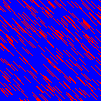
\includegraphics[width=0.2\textwidth]{Figures/bernoulli_cloud/init_condition1.png}
	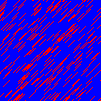
\includegraphics[width=0.2\textwidth]{Figures/bernoulli_cloud/init_condition2.png}
	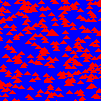
\includegraphics[width=0.2\textwidth]{Figures/bernoulli_cloud/init_condition3.png}
	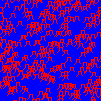
\includegraphics[width=0.2\textwidth]{Figures/bernoulli_cloud/init_condition5.png} \\
	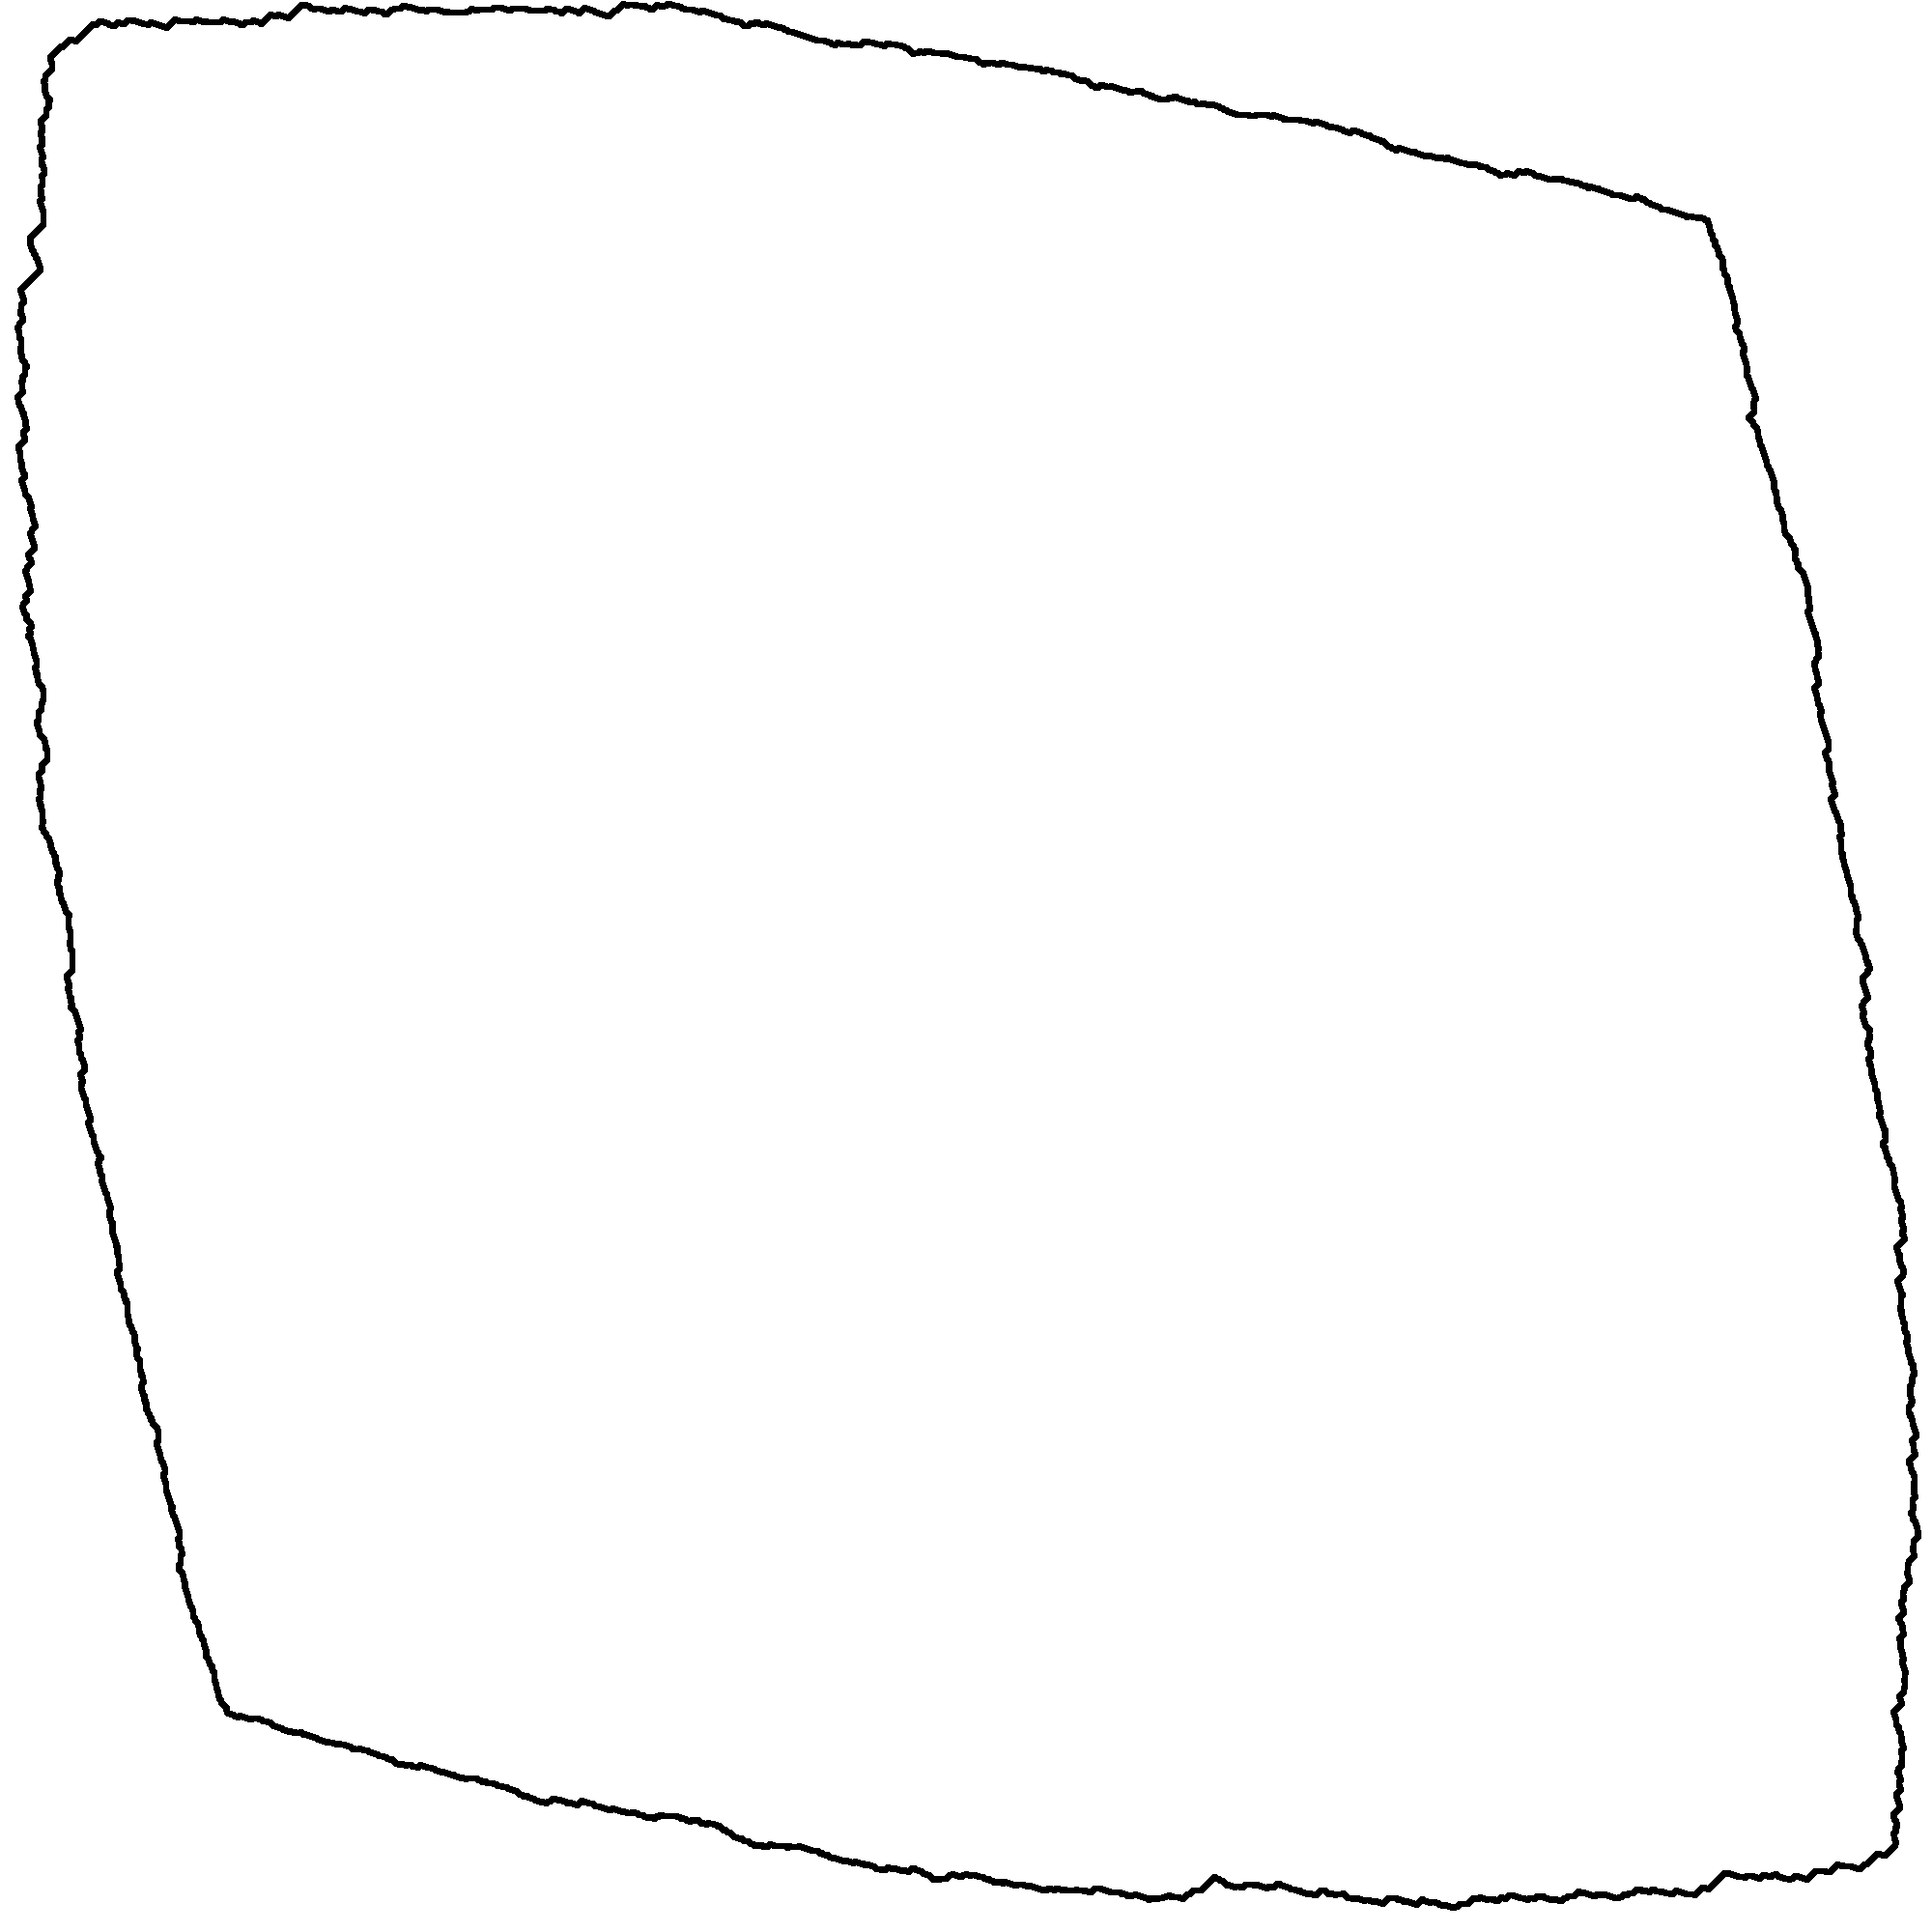
\includegraphics[width=0.2\textwidth]{Figures/bernoulli_cloud/limit_shape1.png}
	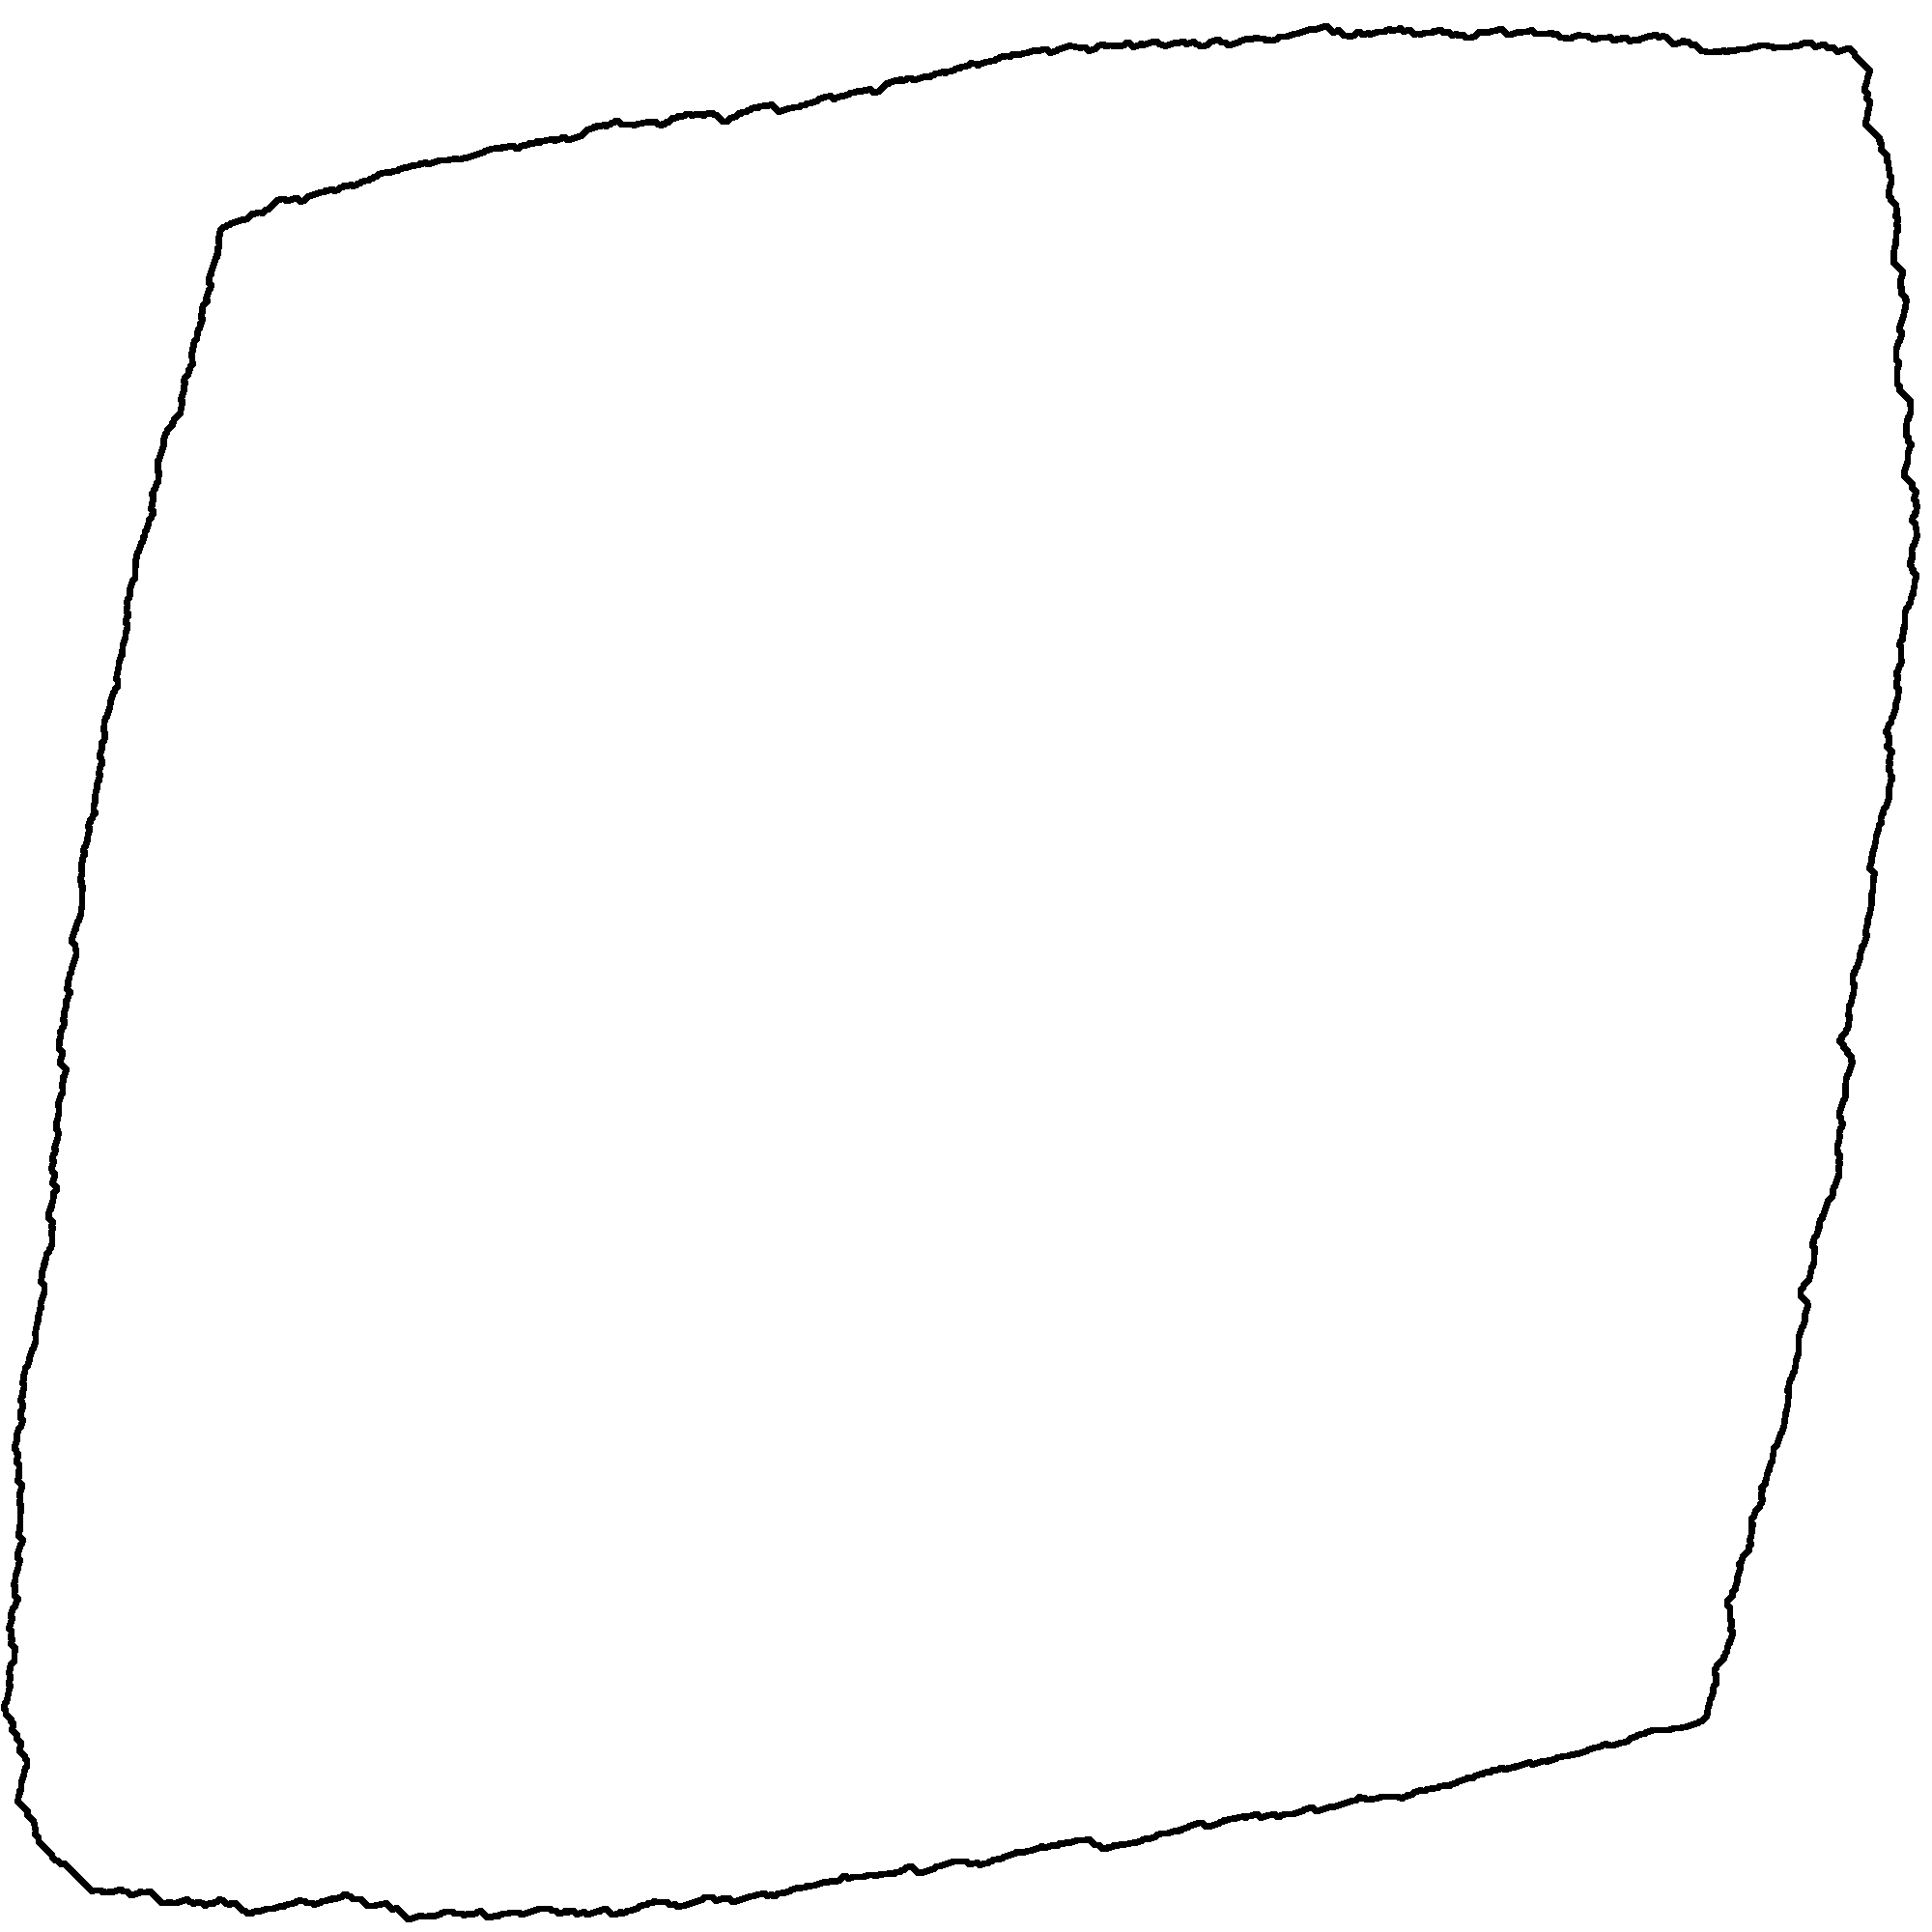
\includegraphics[width=0.2\textwidth]{Figures/bernoulli_cloud/limit_shape2.png}
	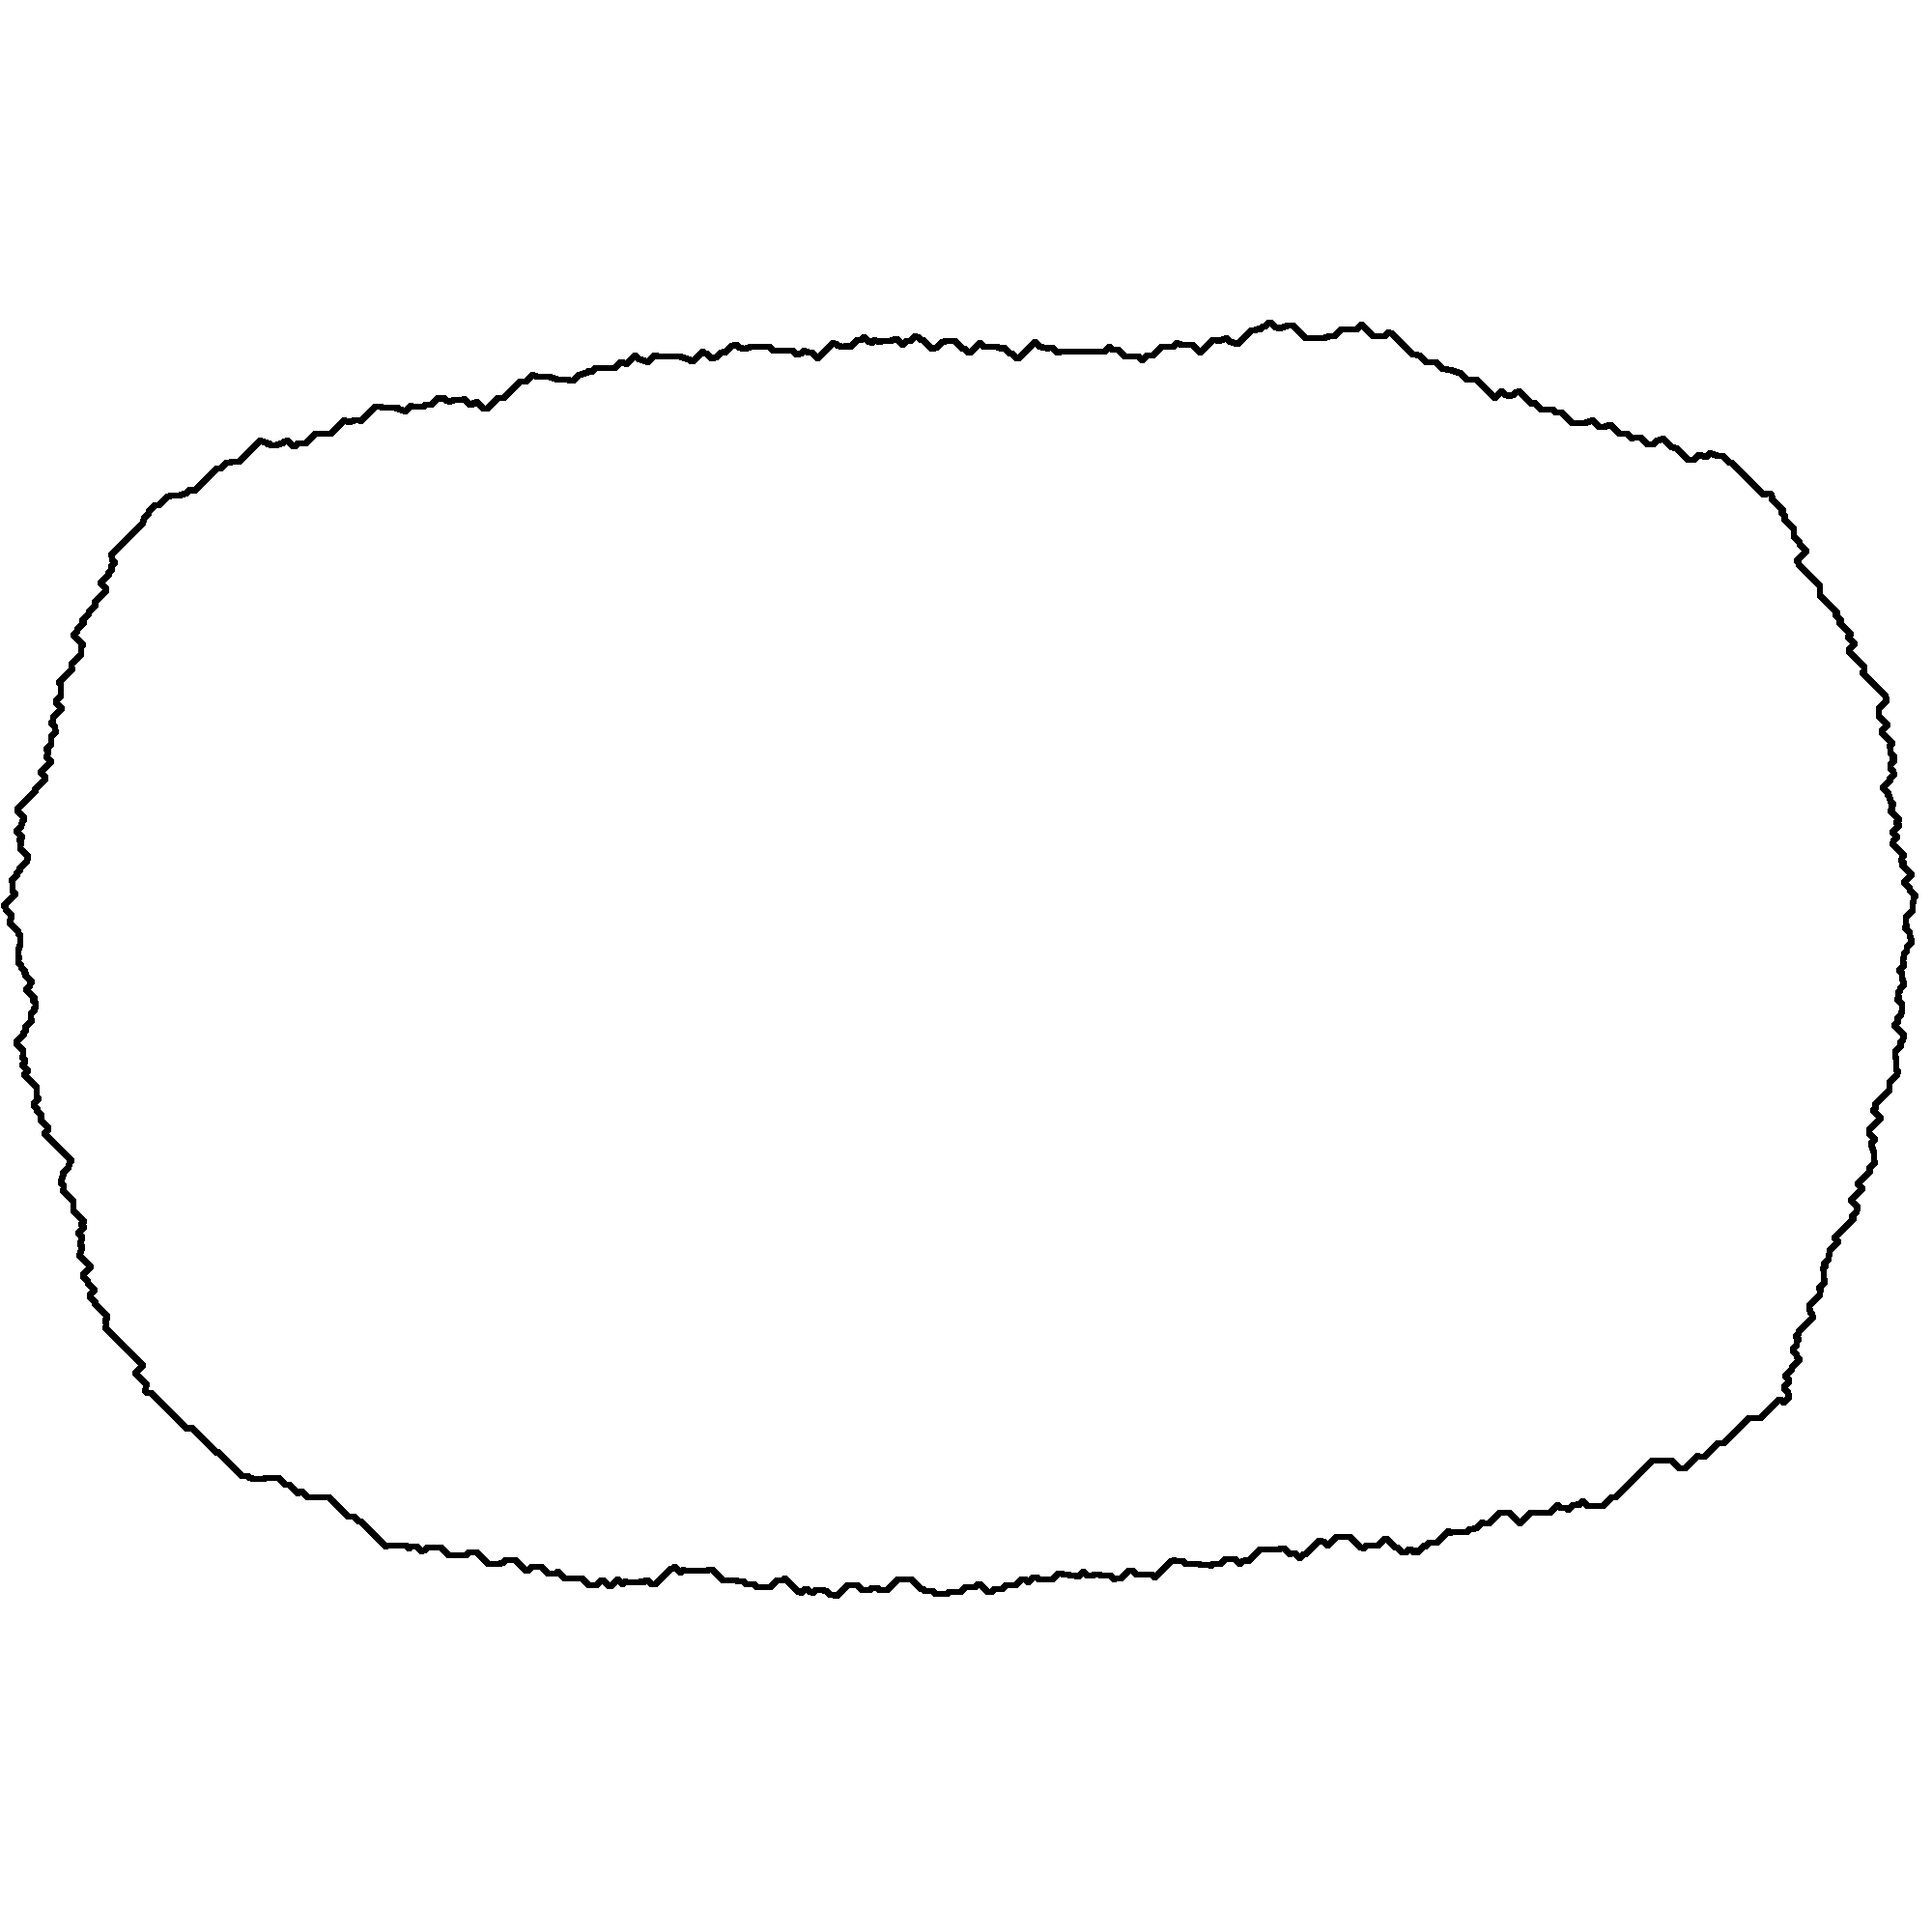
\includegraphics[width=0.2\textwidth]{Figures/bernoulli_cloud/limit_shape3.png}
	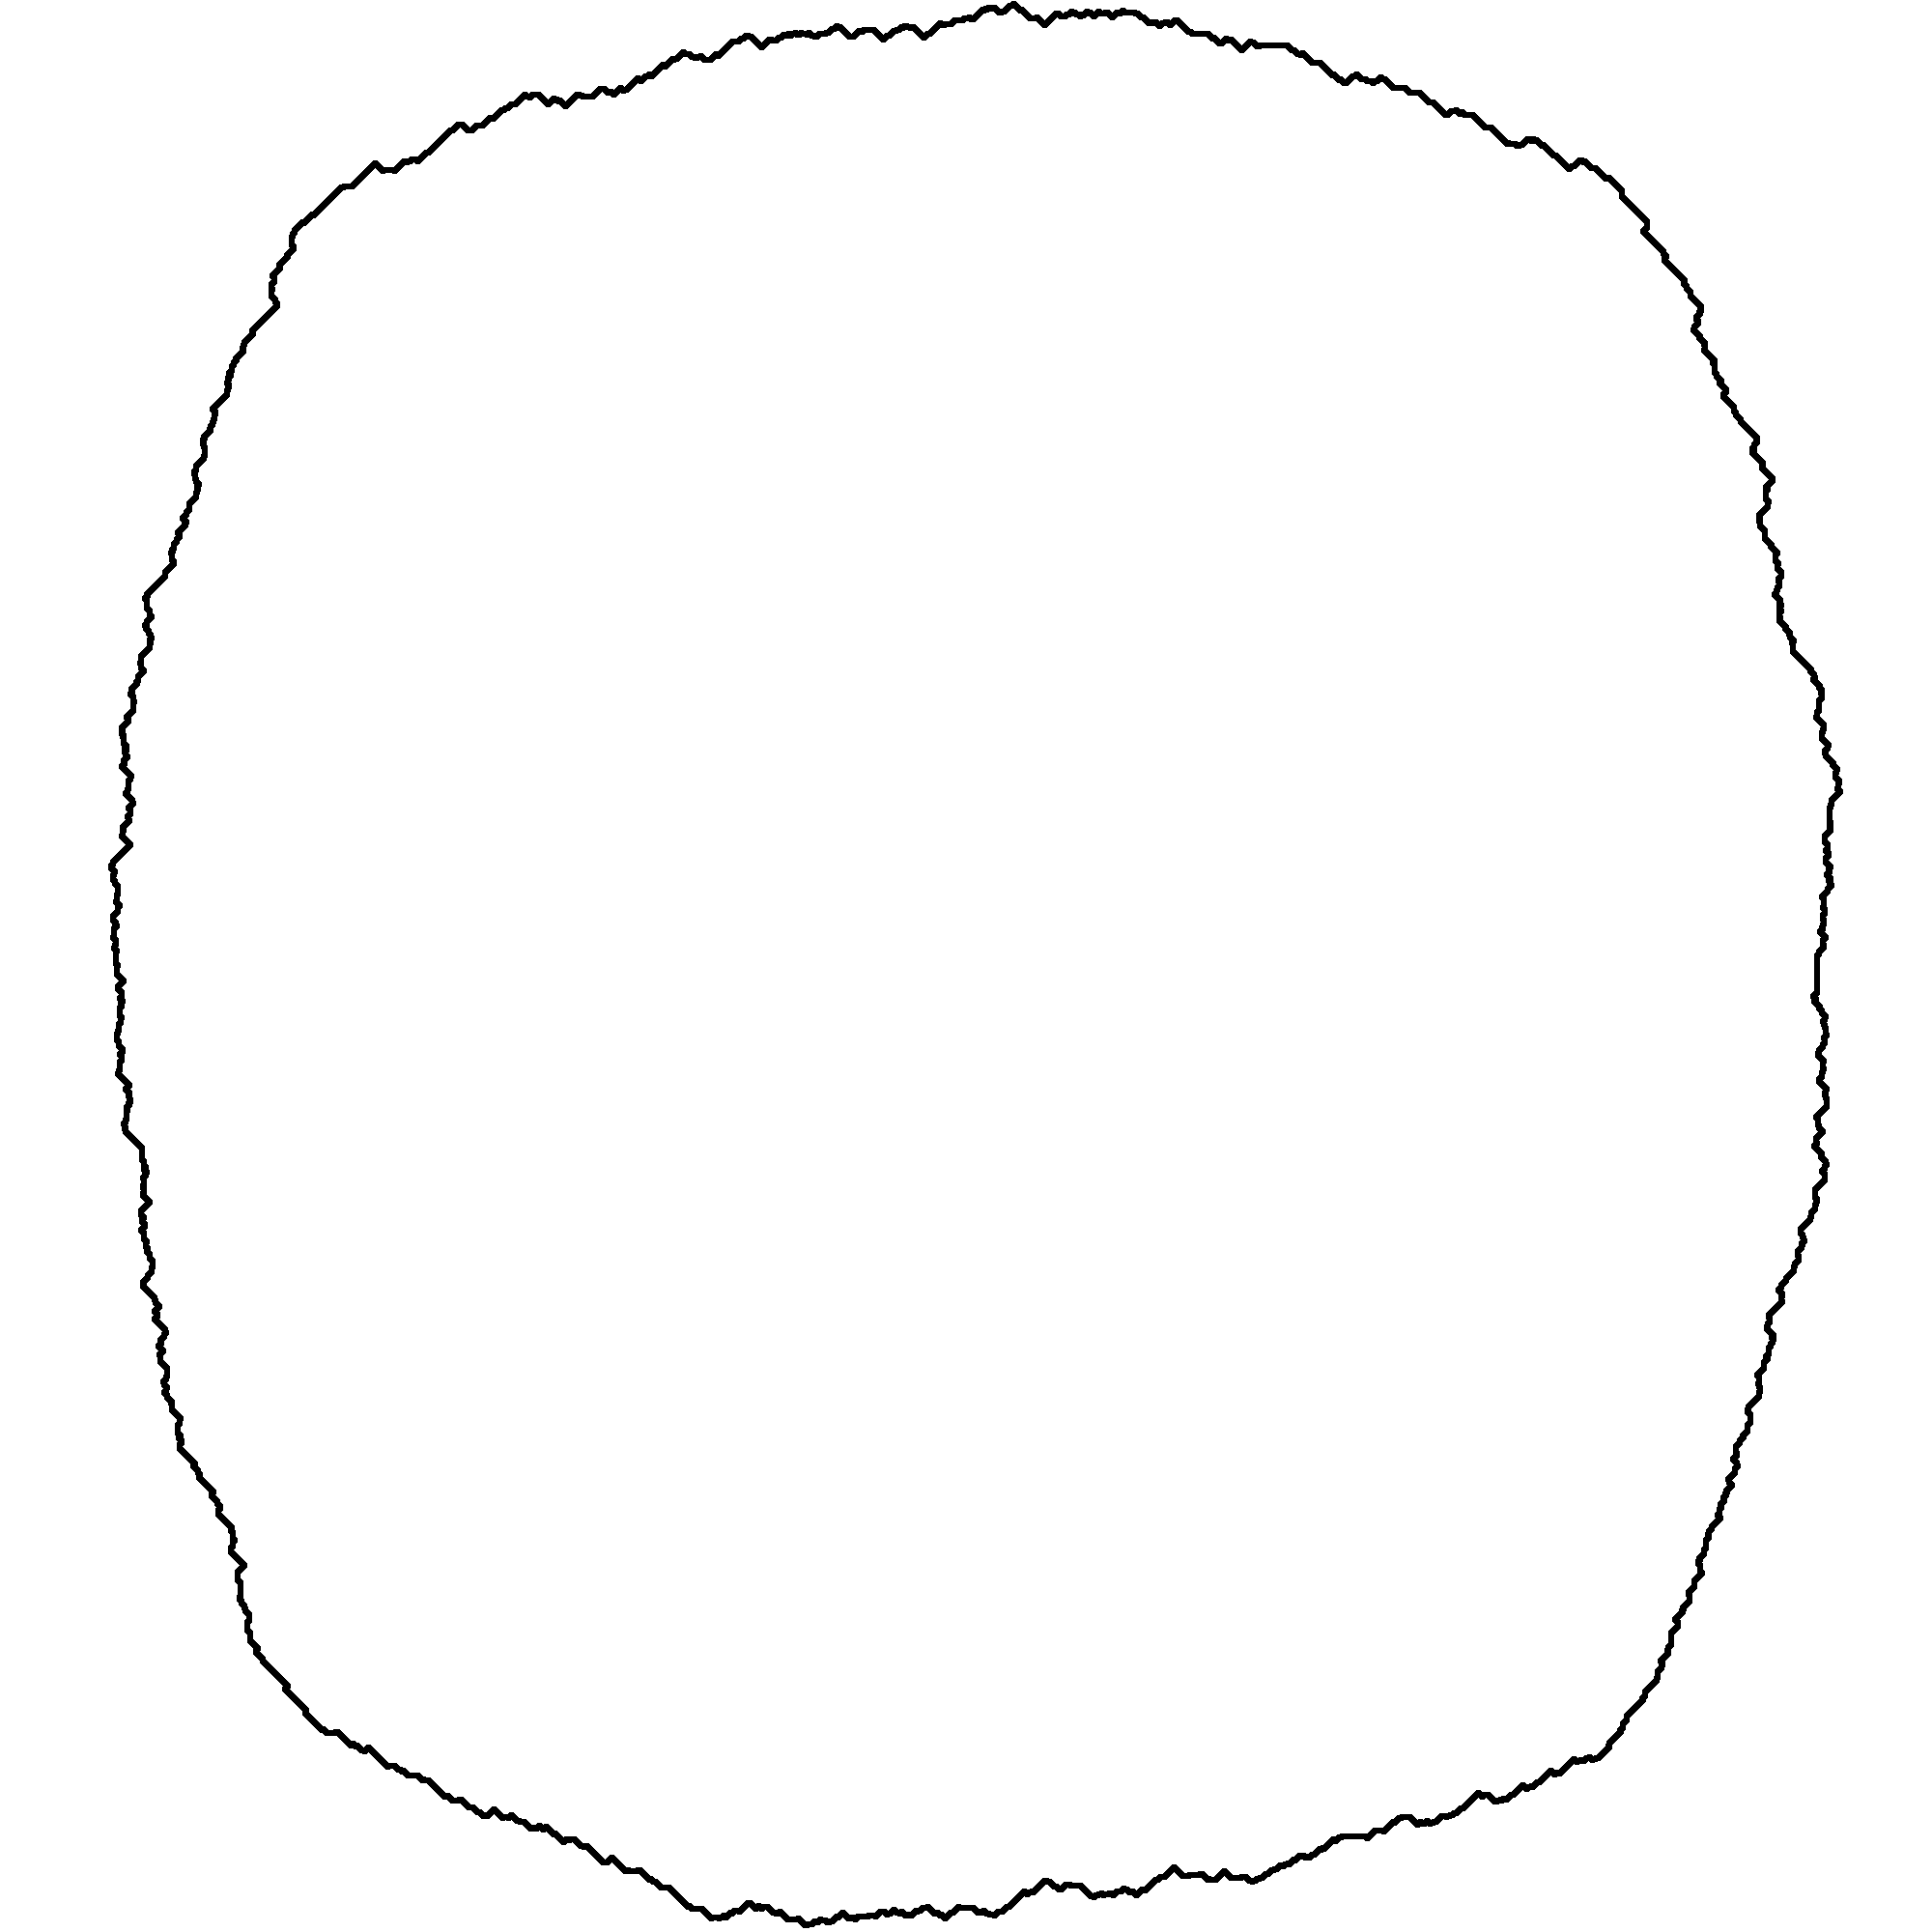
\includegraphics[width=0.2\textwidth]{Figures/bernoulli_cloud/limit_shape5.png}    
	\caption{Initial random backgrounds and computed limit shapes. The random backgrounds
		are built from Bernoulli clouds of the indicated point sets. Blue is 2 chips and red is 3 chips. }
	\label{fig:bernoulli_clouds}
\end{figure} 
\begin{table}
	\begin{tabular}{ c |  c |   c | c | c } \hline
		$\begin{bmatrix} 3 \end{bmatrix}$  & 
		$\begin{bmatrix} 2 & 3 \\
		3 & 2 
		\end{bmatrix}$   &
		$\begin{bmatrix}
		3& 2 & 3 \\ 
		2 & 3 & 3 \\
		3 & 2 & 3 
		\end{bmatrix}$ &
		$\begin{bmatrix}
		2 & 2 & 3  &  3 \\
		3 &  2 &  3 &  2 \\
		2 & 3 & 2 & 2 \\
		2 & 2 &  3 & 2 
		\end{bmatrix}$ &
		$\begin{bmatrix}
		3 & 2 & 3 & 3 & 3 \\
		2 & 2 & 3 & 3 & 3 \\
		2 &  2 & 3 & 2 & 2 \\
		3 & 3 & 2 & 2 & 2 \\
		3 & 3 & 3 & 2 & 3 
		\end{bmatrix}$ 
		\\ \hline
		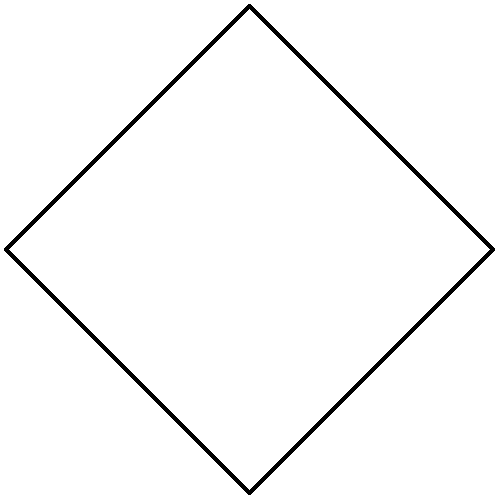
\includegraphics[width=0.15\textwidth]{Figures/checkerboard/1.png} & 	
		
\includegraphics[width=0.14\textwidth]{Figures/checkerboard/2.png} &
		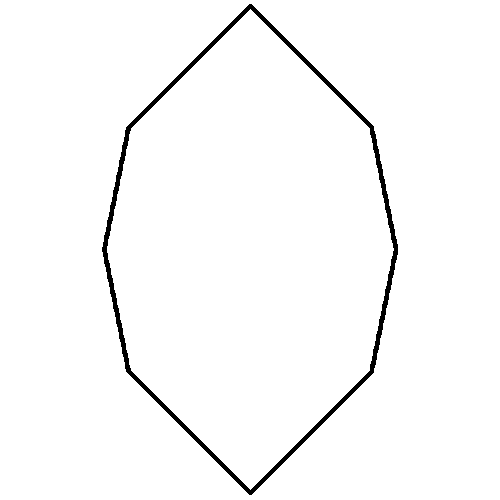
\includegraphics[width=0.15\textwidth]{Figures/checkerboard/3.png} &
		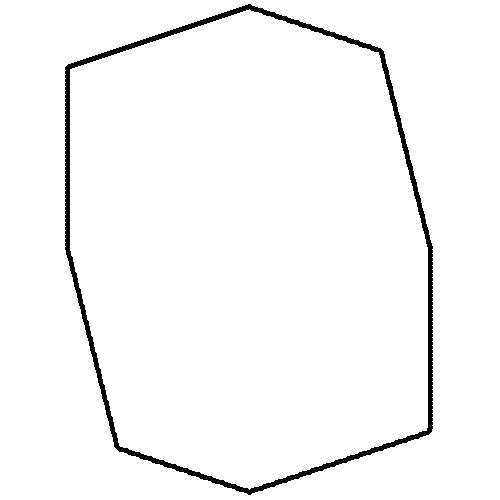
\includegraphics[width=0.15\textwidth]{Figures/checkerboard/4.png} &
		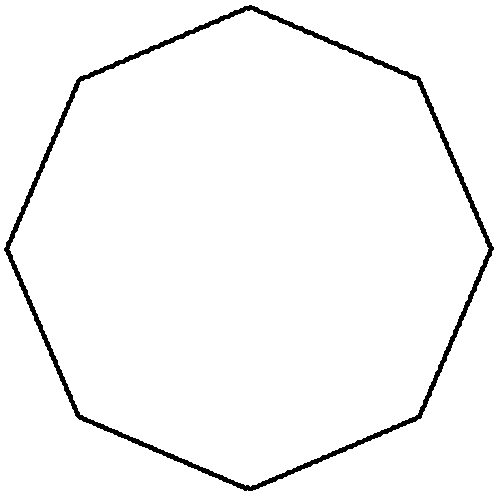
\includegraphics[width=0.15\textwidth]{Figures/checkerboard/5.png} 
		\\ \hline
	\end{tabular}
	\caption{Computed limited shapes of periodic, checkerboard backgrounds of the indicated box.}	
	\label{tab:periodic_exploding_shapes}
\end{table}

\section{Failure of convergence} \label{sec:counterexample}
In this section we construct a family of exploding sandpiles which fail to have a limit shape. 
As the construction indicates, the counterexample is stable: it can be random or periodic. 

\begin{theorem} \label{theorem:counterexample}
	For each dimension $d \geq 2$, there are explosive backgrounds $\eta \not \geq (2d - 2)$ on $\Z^d$ which fail to have a limit shape;
	the first arrival times $\mathcal{T}(n) := \min\{ t > 0 : v_t(n e_1) > 0 \}$ do not converge,
	\begin{equation} \label{eq:counterexample_upper}
	\limsup_{n \to \infty} n^{-1} \mathcal{T}(n) \geq 3/2
	\end{equation}
	and 
	\begin{equation} \label{eq:counterexample_lower}
	\liminf_{n \to \infty} n^{-1} \mathcal{T}(n) = 1.
	\end{equation}
\end{theorem}



\begin{figure}
	
\includegraphics[width=0.4\textwidth]{Figures/counter_example/limit_shape.png}
	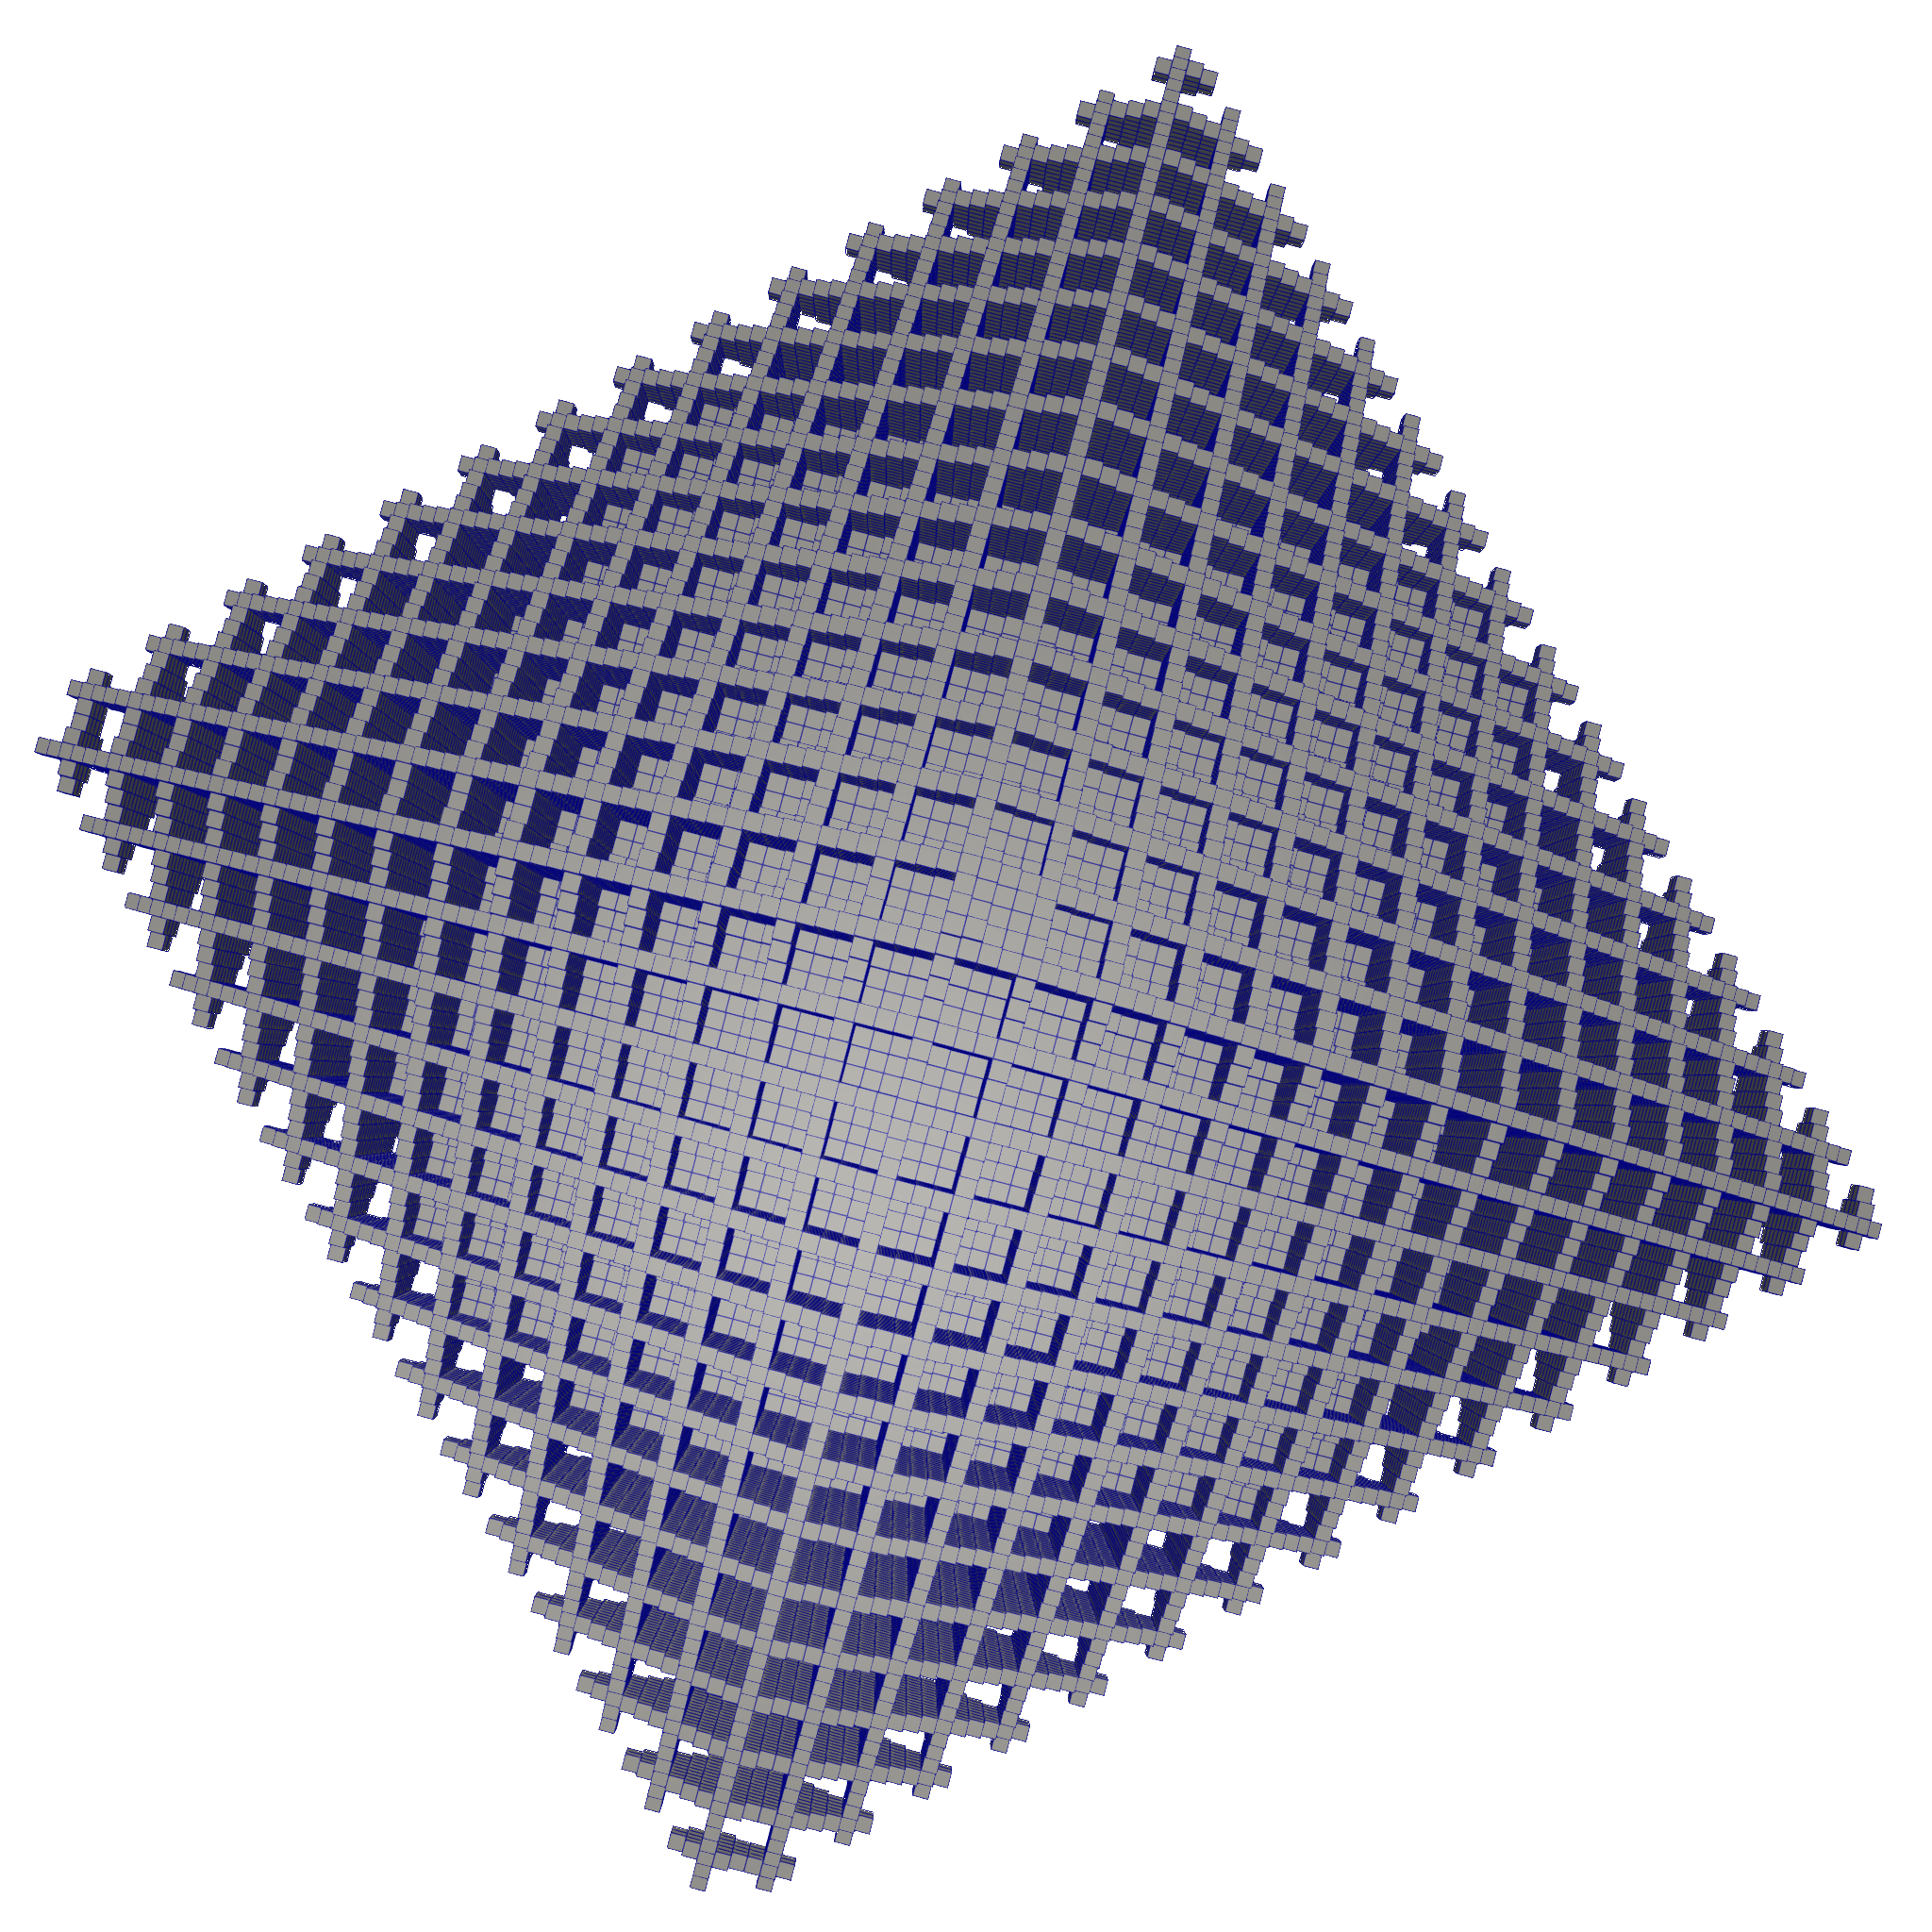
\includegraphics[width=0.4\textwidth]{Figures/counter_example/surface_with_edges.png}
	\caption{The counterexample from Theorem \ref{theorem:counterexample} for $d = 2$ and $d = 3$.}
	\label{fig:counterexample}
\end{figure}

We explicitly demonstrate a family of checkerboard backgrounds which are explosive but do not have a limit shape. Our counterexample is essentially a two-dimensional one. After constructing it in two dimensions, we embed it into higher-dimensions and show failure of convergence by comparison with the two-dimensional counterexample. 


\subsection{Proof of Theorem \ref{theorem:counterexample} for \texorpdfstring{$d=2$}{d=2}} \label{sec:counterexample_2D}
We use the notation of Section \ref{sec:generalization}.  Let $\mathcal{B} := \{ x \in \Z^2 : 0 \leq x \leq 3\}$
denote a box of side length 4 and take $\zeta_1,\zeta_2: \mathcal{B} \to \{1,2, 3\}$ as
\[
\zeta_1 := 
\begin{bmatrix}
1 & 3 & 3 & 1 \\
3 & 3 & 3 & 3 \\
3 & 3 & 3 & 3  \\
1 & 3 & 3 & 1
\end{bmatrix}
\qquad 
\zeta_2 := 
\begin{bmatrix}
1 & 3 & 3 & 1 \\
3 & 2 & 3 & 3 \\
3 & 3 & 3 & 3  \\
1 & 3 & 3 & 1
\end{bmatrix}, 
\]
where the lower-left corner of the box is $(0,0)$ and left-to-right and down-to-up are increasing coordinates.
Let $\eta$ be an arbitrary tiling of $\zeta_1, \zeta_2$; for example, $\eta$ could be a sample from the 
random checkerboard measure. Fix coordinates so that 
\[
\eta(x_1, x_2) = \zeta_i(x_1 \mbox{ mod }  4, x_2  \mbox{ mod }  4).
\]
Let $v_t$ be the sequence of parallel toppling odometers for $s_0 = \eta + 3  \delta_0$. We first verify \eqref{eq:counterexample_lower}.

\subsubsection*{Step 1: Proof of \eqref{eq:counterexample_lower}}
We show for all $n \geq 0$
\begin{equation}
(4 n + 1) \leq \mathcal{T}(4 n + 1) \leq 4 n + 4.
\end{equation} 
By inspection, $v_1(0) = 1$ and $v_2(e_1) = v_2(e_2) = 1$. Now, take $n \geq 1$
and observe that there is a line of 3s connecting $e_2$ to $(e_2 + (4 n + 1)e_1)$.
Thus, $v_{4 n+3}(e_2 + (4 n + 1)e_1) = 1$ and $v_{4 n+4}( (4 n + 1)e_1) = 1$.
The lower bound is immediate from $\eta \leq (2d - 1)$ --- a site can fire only if a neighbor has fired previously.


\subsubsection*{Step 2: $\eta$ is explosive}
By Theorem 2.8 in \cite{fey2009stabilizability}, 
it suffices to construct a toppling procedure
which transforms  $\eta$ into a configuration $\eta'$ which is not stabilizable
in such a way that only sites with at least $2 d$ chips are toppled. 
Start by toppling the origin, then every 3, then every 2, then the $2 \times 2$ box of 1s 
containing the origin,
\[
\eta' := \eta + \Delta \left( 1\{\eta \geq 2\} + \delta_0 + \delta_{-e_1} + \delta_{-e_2} + \delta_{-e_1-e_2} \right).
\]
(It may be checked that this is indeed a legal toppling procedure in the sense of \cite{fey2009stabilizability}.)
The resulting configuration is (away from the origin) a tiling of $\zeta_1',\zeta_2' : \mathcal{B} \to \{2, 3\}$, 
\begin{equation} \label{eq:modified_checkerboard}
\zeta_1' := 
\begin{bmatrix}
3 & 2 & 2 & 3 \\
2 & 3 & 3 & 2 \\
2 & 3 & 3 & 2  \\
3 & 2 & 2 & 3
\end{bmatrix}
\qquad 
\zeta_2' := 
\begin{bmatrix}
3 & 2 & 2 & 3 \\
2 & 2 & 3 & 2 \\
2 & 3 & 3 & 2  \\
3 & 2 & 2 & 3
\end{bmatrix}.
\end{equation}
\begin{remark}
	The reason why convergence fails for this counterexample is that the limit 
	shape of the explosive background $\eta'$ is not a diamond. See Figure \ref{fig:counterexample}.
	When $d=2$ the limit shape is a regular octagon with boundary $\max(|x-y/3|, |x+y/3|, |x/3 - y|, |x/3 + y|)$, but we will not prove this. 
\end{remark}

Both $\zeta_1'$ and $\zeta_2'$ are box-crossing, so it remains to check 
that we can construct a sequence of firings to the outer face
of a box away from the origin. The box containing
the origin is at least
\[
\eta'|_{[0,3]^2} \geq
\begin{bmatrix}
3 & 2 & 2 & 3 \\
2 & 2 & 3 & 2 \\
3 & 3 & 3 & 2 \\
1 & 3 & 2 & 3
\end{bmatrix}.
\]
From this we see that $3  \delta_0 + \eta'$ is not stabilizable --- in a finite number of steps every site in $[0,3]^2$ will fire. 

\subsubsection*{Step 3: Reductions}
Before proving \eqref{eq:counterexample_upper}, we make several reductions.
We seek to lower bound $\mathcal{T}$, therefore, we are free to add
to $\eta$ as this will only decrease the arrival time. First, we may suppose all of the boxes are $\zeta_1$ rather then $\zeta_2$. 

We then increment the background so as to reduce to a sandpile on a cylinder,  $\mathcal{C} := \{ x \in \Z^2 : x_1 \geq 0,  3 \geq x_2 \geq 0\}$. 
Specifically, let $\zeta: \mathcal{C} \to \{1, 3, 4\}$, 
\[
\zeta := 
\begin{bmatrix}
\begin{matrix}
1 & 3 & 3 & 1 \\
3 & 3 & 3 & 3 \\
3 & 3 & 3 & 3 \\
4 & 3 & 3 & 1 
\end{matrix}
& \zeta_1 & \zeta_1 & \cdots
\end{bmatrix}
\]
with the origin, $(0,0)$, on the bottom left with left-to-right, down-to-up 
increasing.  To 
periodically tile by $\zeta$: set for $x_1 \geq 0$, 
\[
\hat{\eta}(x_1, x_2) :=
\zeta(x_1, x_2 \mbox{ mod } 4)
\]
and for $x_1 < 0$, 
\[
\hat{\eta}(x_1, x_2) := \hat{\eta}(-(x_1+1), x_2).
\]
Note that $\hat{\eta} \geq \eta$. 

The structure of $\hat{\eta}$ allows us to reduce
to a symmetrized Laplacian on the cylinder $\mathcal{C}$ (see for example Lemma 2.3 in \cite{bou2020dynamic}) with reflecting boundaries at $x_1 = 0$: $v_t(-1, x_2) = v_t(0,x_2)$
and torus boundary conditions for $x_2 \in \{0,3\}$: $v_t(x_1, -1) = v_t(x_1,3)$, and $v_t(x_1, 4) = v_t(x_1,0)$.  This defines the {\it symmetrized} Laplacian $\Delta$ and nearest neighbors $y \sim x$ on $\mathcal{C}$. 

Let $\tilde{u}(x): \mathcal{C} \to \{0 ,1\}$ be  $\tilde{u}(x) := 1 \{ \hat{\eta}(x) \geq 3\}$.
Then, 
\[
\Delta \tilde{u} + \zeta
=
\begin{bmatrix}
\begin{matrix}
4 & 2 & 2 & 3 \\
2 & 3 & 3 & 2 \\
3 & 3 & 3 & 2 \\
3 & 3 & 2 & 3 
\end{matrix}
& \zeta_1' & \zeta_1' & \cdots 
\end{bmatrix}
=: \zeta'.
\]
Let $v_t: \mathcal{C} \to \Z^+$ be the symmetrized parallel toppling odometer for $\zeta$ and $w_t:\mathcal{C} \to \Z^+$ the
same for $\hat{\eta}'$ (defined with $\zeta'$ as $\hat{\eta}$ was with $\zeta$). We claim that 
\begin{equation} \label{eq:second_limit_reduction}
\mathcal{T}'(3 + 8n) \leq \mathcal{T}(3 + 8 n), 
\end{equation}
where $\mathcal{T}'(n) := \min\{t > 0 : w_t(n e_1) > 0\}$.
In fact, we claim
\begin{equation} \label{eq:topple_compare_induc}
v_t \leq w_t + \tilde{u}
\end{equation}
for all $t \geq 0$.  This includes \eqref{eq:second_limit_reduction} as $\tilde{u}( (3 + 8 n) e_1) = 0$. 
We observe \eqref{eq:topple_compare_induc} is a consequence of induction: the base case $t = 0$ is automatic and 
the inductive step is, 
\begin{align*}
v_{t+1}(x) &=  \lfloor \frac{\sum_{y \sim x}  v_t(y) + \zeta(x)}{4} \rfloor  \\
&\leq  \lfloor \frac{\sum_{y \sim x}  (w_t(y) + \tilde{u}(y)) + \zeta(x)}{4} \rfloor  \\
&= \tilde{u}(x) +  \lfloor \frac{\sum_{y \sim x}  w_t(y) + \Delta \tilde{u}(x) + \zeta(x)}{4} \rfloor  \\
&= \tilde{u}(x) +  w_{t+1}(x).
\end{align*}

\subsubsection*{Step 4: Proof of \eqref{eq:counterexample_upper}}
We show for all $n \geq 1$,
\begin{equation} \label{eq:second_limit_upper_bound}
\mathcal{T}'(3 + 8 n) \geq 12 n.
\end{equation}
We do so by building a `pulsating front' for $w_t$ in the horizontal direction. (Readers interested in pulsating fronts in periodic media on $\R^d$ may see Section 2.2 of \cite{xin2009introduction}.)


We first reduce to the last-wave for $w_t$, $\hat{w}_t$, with initial conditions
$\hat{w}_0 = \delta_{(0,3)}$ and
$\hat{s}_0 = \zeta' + \Delta \hat{w}_0$. The justification is identical to Step 1 of the proof of Proposition \ref{prop:approximate_subadditive}
and so is omitted.  Using $\hat{w}_t \leq 1$, we make another reduction to initial condition
$\hat{w}_0: \mathcal{C} \to \{0, 1\}$, 
\[
\hat{w}_0 = 
\begin{bmatrix} 
\begin{smallmatrix}
1 & 1 & 1 & 1 \\
1 & 1 & 1 & 0 \\
1 & 1 & 1 & 0 \\
1 & 1 & 1 & 1 
\end{smallmatrix}
& \mathbf{0} & \mathbf{0} & \cdots
\end{bmatrix}.
\]
\setcounter{MaxMatrixCols}{50}
We now show, by manual computation, that the configuration of the odometer at the front, the rightmost $4 \times 4$ box in $\mathcal{C}$ containing a site which has toppled, 
is 12-periodic in time. For notational ease, we denote sites which have toppled by $*$, 
\begin{align*}
\hat{s}_0 &= 
\begin{bmatrix}
\begin{smallmatrix}
* & * & * & * & 4 & 2 & 2 & 3 & 3 & 2 & 2 & 3  & 3 \\
* & * & * & 4 & 2 & 3 & 3 & 2 & 2 & 3 & 3 & 2 & 2 \\
* & * & * & 4 & 2 & 3 & 3 & 2 & 2 & 3 & 3 & 2 & 2 \\ 
* & * & * & * & 4 & 2 & 2 & 3 & 3 & 2 & 2 & 3 & 3
\end{smallmatrix}
& 
\cdots
&
\end{bmatrix}
\qquad
\hat{s}_7 = 
\begin{bmatrix}
\begin{smallmatrix}
* & * & * & * & * & * & * & * & * & 3 & 2 & 3 & 3 \\
* & * & * & * & * & * & * & * & 4 & 3 & 3 & 2 & 2  \\
* & * & * & * & * & * & * & * & 4 & 3 & 3 & 2 & 2 \\
* & * & * & * & * & * & * & * & * & 3 & 2 & 3 & 3
\end{smallmatrix}
& 
\cdots
&
\end{bmatrix} \\
\hat{s}_1 &= 
\begin{bmatrix}
\begin{smallmatrix}
* & * & * & * & * & 3 & 2 & 3 & 3 & 2 & 2 & 3 & 3 \\ 
* & * & * & * & 4 & 3 & 3 & 2 & 2 & 3 & 3 & 2 & 2 \\
* & * & * & * & 4 & 3 & 3 & 2 & 2 & 3 & 3 & 2 & 2 \\
* & * & * & * & * & 3 & 2 & 3 & 3 & 2 & 2 & 3 & 3
\end{smallmatrix}
& 
\cdots
&
\end{bmatrix} 
\qquad \hat{s}_8 =
\begin{bmatrix}
\begin{smallmatrix}
* & * & * & * & * & * & * & * & * & 3 & 2 & 3 & 3 \\ 
* & * & * & * & * & * & * & * & * & 4 & 3 & 2 & 2 \\ 
* & * & * & * & * & * & * & * & * & 4 & 3 & 2 & 2 \\ 
* & * & * & * & * & * & * & * & * & 3 & 2 & 3 & 3
\end{smallmatrix}
& 
\cdots
&
\end{bmatrix} \\
\hat{s}_2 &= 
\begin{bmatrix}
\begin{smallmatrix}
* & * & * & * & * & 3 & 2 & 3 & 3 & 2 & 2 & 3 & 3 \\
* & * & * & * & * & 4 & 3 & 2 & 2 & 3 & 3 & 2 & 2 \\ 
* & * & * & * & * & 4 & 3 & 2 & 2 & 3 & 3 & 2 & 2 \\
* & * & * & * & * & 3 & 2 & 3 & 3 & 2 & 2 & 3 & 3
\end{smallmatrix}
& 
\cdots
&
\end{bmatrix} 
\qquad \hat{s}_9 =
\begin{bmatrix}
\begin{smallmatrix}
* & * & * & * & * & * & * & * & * & 4 & 2 & 3 & 3 \\ 
* & * & * & * & * & * & * & * & * & * & 4 & 2 & 2 \\ 
* & * & * & * & * & * & * & * & * & * & 4 & 2 & 2 \\
* & * & * & * & * & * & * & * & * & 4 & 2 & 3 & 3
\end{smallmatrix}
& 
\cdots
&
\end{bmatrix} \\
\hat{s}_3 &= 
\begin{bmatrix}
\begin{smallmatrix}
* & * & * & * & * & 4 & 2 & 3 & 3 & 2 & 2 & 3 & 3 \\ 
* & * & * & * & * & * & 4 & 2 & 2 & 3 & 3 & 2 & 2 \\
* & * & * & * & * & * & 4 & 2 & 2 & 3 & 3 & 2 & 2 \\
* & * & * & * & * & 4 & 2 & 3 & 3 & 2 & 2 & 3 & 3
\end{smallmatrix}
& 
\cdots
&
\end{bmatrix} 
\qquad \hat{s}_{10} = 
\begin{bmatrix}
\begin{smallmatrix}
* & * & * & * & * & * & * & * & * & * & 4 & 3 & 3 \\ 
* & * & * & * & * & * & * & * & * & * & * & 3 & 2 \\ 
* & * & * & * & * & * & * & * & * & * & * & 3 & 2 \\ 
* & * & * & * & * & * & * & * & * & * & 4 & 3 & 3
\end{smallmatrix}
& 
\cdots
&
\end{bmatrix} \\
\hat{s}_4 &= 
\begin{bmatrix}
\begin{smallmatrix}
* & * & * & * & * & * & 4 & 3 & 3 & 2 & 2 & 3 & 3 \\ 
* & * & * & * & * & * & * & 3 & 2 & 3 & 3 & 2 & 2 \\ 
* & * & * & * & * & * & * & 3 & 2 & 3 & 3 & 2 & 2 \\ 
* & * & * & * & * & * & 4 & 3 & 3 & 2 & 2 & 3 & 3
\end{smallmatrix}
& 
\cdots
&
\end{bmatrix}
\qquad \hat{s}_{11} = 
\begin{bmatrix}
\begin{smallmatrix}
* & * & * & * & * & * & * & * & * & * & * & 4 & 3 \\ 
* & * & * & * & * & * & * & * & * & * & * & 3 & 2 \\
* & * & * & * & * & * & * & * & * & * & * & 3 & 2 \\
* & * & * & * & * & * & * & * & * & * & * & 4 & 3
\end{smallmatrix}
& 
\cdots
&
\end{bmatrix} \\
\hat{s}_5 &= 
\begin{bmatrix}
\begin{smallmatrix}
* & * & * & * & * & * & * & 4 & 3 & 2 & 2 & 3 & 3 \\ 
* & * & * & * & * & * & * & 3 & 2 & 3 & 3 & 2 & 2 \\ 
* & * & * & * & * & * & * & 3 & 2 & 3 & 3 & 2 & 2 \\ 
* & * & * & * & * & * & * & 4 & 3 & 2 & 2 & 3 & 3
\end{smallmatrix}
& 
\cdots
&
\end{bmatrix} 
\qquad \hat{s}_{12} = 
\begin{bmatrix}
\begin{smallmatrix}
* & * & * & * & * & * & * & * & * & * & * & *  & 4 \\
* & * & * & * & * & * & * & * & * & * & * & 4  & 2 \\
* & * & * & * & * & * & * & * & * & * & * & 4 &  2 \\ 
* & * & * & * & * & * & * & * & * & * & * & * & 4
\end{smallmatrix}
& 
\cdots
&
\end{bmatrix}. \\
\hat{s}_6 &= 
\begin{bmatrix}
\begin{smallmatrix}
* & * & * & * & * & * & * & * & 4 & 2 & 2 & 3 & 3 \\ 
* & * & * & * & * & * & * & 4 & 2 & 3 & 3 & 2 & 2 \\ 
* & * & * & * & * & * & * & 4 & 2 & 3 & 3 & 2 & 2 \\ 
* & * & * & * & * & * & * & * & 4 & 2 & 2 & 3 & 3
\end{smallmatrix}
& 
\cdots
&
\end{bmatrix}
\end{align*}

This shows that
\[
\hat{w}_{12} = 
\begin{bmatrix}
\begin{smallmatrix}
1 & 1 & 1 & 1 & 1 & 1 & 1 & 1 & 1 & 1 & 1 & 1 \\ 
1 & 1 & 1 & 1 & 1 & 1 & 1 & 1 & 1 & 1 & 1 & 0 \\ 
1 & 1 & 1 & 1 & 1 & 1 & 1 & 1 & 1 & 1 & 1 & 0 \\ 
1 & 1 & 1 & 1 & 1 & 1 & 1 & 1 & 1 & 1 & 1 & 1
\end{smallmatrix}
& 
\mathbf{0} 
&
\mathbf{0} 
& \cdots
\end{bmatrix},
\]
so the odometer at the front is identical to what it was at the start and the process `resets'. Hence, 
by induction on $n\geq1$,
\begin{equation}
\hat{T}(3 + 8 n) = 12 n\,,
\end{equation}
where $\hat{T}(n) := \min\{ t > 0 : \hat{w}_t(n e_1) > 0 \}$. 
This implies  \eqref{eq:second_limit_upper_bound}, completing the proof by \eqref{eq:second_limit_reduction}.



\subsection{Proof of Theorem \ref{theorem:counterexample} for \texorpdfstring{$d \geq 3$}{d > 2}} \label{sec:proof_of_generalization}
Let $\eta^{(2D)}: \Z^2 \to \{1, 2, 3\}$ be the (possibly random) background defined in Section \ref{sec:counterexample_2D} and let $d \geq 3$ be given. Our higher-dimensional counterexample $\eta: \Z^d \to \{ 2 d - 3, 2 d -2, 2 d - 1\}$
is built by stacking the two-dimensional one, 
\begin{equation} \label{eq:stacked_tiling1}
\eta(x_1, x_2, \ldots, x_d) = 2  (d- 2) + \eta^{(2D)}(x_1, x_2) \mbox{ for all $x \in \Z^d$}.
\end{equation}
\subsubsection*{Step 1: Proof of \eqref{eq:counterexample_lower}}
The argument is identical to $d = 2$. 



\subsubsection*{Step 2: $\eta$ is explosive}

Let ${\eta'}^{(2D)}$ be the tiling of $\zeta_1', \zeta_2'$, defined in \eqref{eq:modified_checkerboard}.
The higher-dimensional analogue, $\eta': \Z^d \to \{ 2 d - 3, 2 d -2, 2 d - 1\}$ is also stacked, 
\begin{equation} \label{eq:stacked_tiling2}
\eta'(x_1, x_2, \ldots, x_d) := {\eta'}^{(2D)}(x_1, x_2) + 2  (d - 2).
\end{equation}
The argument is as before: we construct a toppling procedure that transforms $\eta$ into $\eta'$. Since $3  \delta_0 + \eta' \geq (2 d - 2)$ is box-crossing, it is not stabilizable. 

Topple the origin, all sites with $(2d - 1)$ chips, then all sites with $(2d - 2)$, then the column of $(2 d-3)$ near the origin. Let $\tilde{u}$ denote the odometer for this and $\tilde{u}^{(2D)}$ the two-dimensional version and observe that $\tilde{u}(x_1, x_2, \ldots, x_d) = \tilde{u}^{(2D)}(x_1,x_2)$. This implies,
\begin{align*}
&\sum_{i=1}^{d} (\tilde{u}(x-e_i) + \tilde{u}(x+e_i) - 2 \tilde{u}(x)) + \eta \\
&= \sum_{i=1}^2 (\tilde{u}^{(2D)}(x-e_i) + \tilde{u}^{(2D)}(x+e_i) - 2 \tilde{u}^{(2D)}(x)) + \eta \\
&= \sum_{i=1}^2 (\tilde{u}^{(2D)}(x-e_i) + \tilde{u}^{(2D)}(x+e_i) - 2 \tilde{u}^{(2D)}(x)) + \eta^{(2D)} + 2  (d-2) \\
&= {\eta'}^{(2D)} + 2  (d-2) \\
&= \eta'. 
\end{align*}
We conclude by observing $\eta'$ is box-crossing as $3  \delta_0 + \eta' \geq (2 d - 2)$ and every layer in the box  $\mathbf{B}^{(d)} := \{ x \in \Z^d : 0 \leq x \leq 3 \}$, contains at least one site with $(2 d - 1)$ chips. Indeed, for all $(3, 3, \mathbf{x}_{d-2}) \in \mathbf{B}^{(d)}$, 
\[
\eta'(3,3, \mathbf{x}_{d-2}) = {\eta'}^{(2D)}(3, 3) + 2  (d - 2) = (2 d - 1),
\]
and every layer in ${\eta'}^{(2D)}$ has at least one site with 3 chips. 




\subsubsection*{Step 3: Proof of \eqref{eq:counterexample_upper}}
Let $v_t^{(2D)}$ be the parallel toppling odometer for $\eta^{(2D)}$. By \eqref{eq:second_limit_upper_bound}
it suffices to show that
\begin{equation} \label{eq:parabolic_least_action}
v_t(x_1, x_2, \ldots, x_d) \leq v_t^{(2D)}(x_1,x_2). 
\end{equation}
This is a consequence of the parabolic least action principle (Lemma 2.3 in \cite{bou2020dynamic}) but 
we provide a self-contained proof here:

Suppose \eqref{eq:parabolic_least_action} holds at time $t$ and we want to show it holds at $(t+1)$.
Let $x$ be given. If $v_t(x) < v_t^{(2D)}(x_1,x_2)$ we are done. Hence, we may suppose $v_t(x) = v_t^{(2D)}(x_1,x_2)$
and 
\[
\Delta v_t(x) + \eta = \sum_{i=1}^d (v_t(x + e_i) + v_t(x - e_i) - 2 v_t(x)) + \eta \geq 2 d.
\]
By \eqref{eq:parabolic_least_action} at time $t$, this implies 
\[
\sum_{i=1}^2 (v_t^{(2D)}((x_1,x_2) + e_i) + v_t^{(2D)}((x_1,x_2) - e_i) - 2 v_t^{(2D)}(x_1,x_2)) + \eta \geq 2 d,
\]
and by \eqref{eq:stacked_tiling1}, 
\[
\Delta v_t^{(2D)}(x_1,x_2) + \eta^{(2D)}(x_1,x_2) \geq 2 d - 2  (d - 2) = 4,
\]
completing the proof.

To verify failure of convergence in the volume sense of Theorem~\ref{theorem:limit_shape}, choose the periodic two-dimensional background obtained by using $\zeta_1$ in every tile, and for $d\geq3$ extend it by \eqref{eq:stacked_tiling1}. For integer $t\geq1$, write $A_t=\{y\in\R^d:\bar v_t(y)>0\}$ and $a_n=3+8n$.
For every $n\geq1$, $k\in\Z$, and $z\in\Z^{d-2}$, the cylinder comparison, followed by~\eqref{eq:parabolic_least_action} when $d\geq3$, gives
\begin{equation*}
v_t(a_n,4k,z)=0\qquad(t<12n)\,.
\end{equation*}
When $d=2$, $z$ is the empty tuple in $\Z^0$, $\|z\|_1=0$, and trailing empty coordinates below are omitted.
The site $e_2$ has fired by time $2$. The nearest-neighbor path from $e_2$ through $(1,1,0)$, $(1,4k+1,0)$, and $(1,4k+1,z)$ to $(a_n,4k+1,z)$ has $a_n+|4k|+\|z\|_1$ edges. Every site after $e_2$ on this path has background height $2d-1$, so
\begin{equation*}
v_{a_n+|4k|+\|z\|_1+2}(a_n,4k+1,z)>0\,.
\end{equation*}
Fix $\varepsilon_d=1/(100d)$ and $\Omega_d=\{y\in\R^d:3/4<y_1<4/5,\ |y_i|<\varepsilon_d\ (2\leq i\leq d)\}$.
For all sufficiently large integers $t$, a fixed positive proportion of the nearest-site cells in an interior box of $\Omega_d$ have centers $(a_n,4k,z)$ and satisfy $t<12n$ and $a_n+|4k|+\|z\|_1+2\leq t$. The congruence conditions on the first two coordinates have density $1/32$, and there is no restriction on the remaining coordinates. Each such cell is absent from $A_t$, while its translate by $e_2/t$ is present. Hence, for some $c_d>0$,
\begin{equation*}
\left|(A_t\triangle(A_t-e_2/t))\cap\Omega_d\right|\geq c_d
\qquad\text{for all sufficiently large integers }t\,.
\end{equation*}
If $|A_t\triangle B|\to0$ for a measurable set $B$, then the triangle inequality and local $L^1$ continuity of translation give $|(A_t\triangle(A_t-e_2/t))\cap\Omega_d|\to0$, a contradiction.

\section{A criterion for exploding} \label{sec:criteria}

For Proposition~\ref{prop:explosion_criteria}, let $(\Omega,\mathcal F,\mathbf P)$ be the bounded-background probability space of Section~\ref{sec:generalization}. The criterion below is applied, in the proof of Theorem~\ref{theorem:explosive}, to the field $\alpha_d$ defined there.
For a finite domain $V \subset \Z^d$, we say  $\eta: V \to \Z$ is {\it recurrent} if the firing of $\partial V$ causes every site in $V$ to eventually topple. Specifically, the $V^c$-frozen parallel toppling odometer for initial conditions $w_0 = 1\{ x \in \partial V\}$, $s_0' = \eta + \Delta w_0$, is eventually 1 on $V$: $w_t |_{V} = 1$ for $t \geq |V|$. We say $\eta: \Z^d \to \Z$ is recurrent if its restriction to $V$ is recurrent for every finite $V \subset \Z^d$.  The measure $\mathbf{P}$ is recurrent if $\mathbf{P}(\mbox{$\eta$ is recurrent}) = 1$. The following criterion follows from recurrence, finite-range dependence, and box-crossing.

\begin{prop} \label{prop:explosion_criteria}
	Let $d\geq2$. If Hypotheses~\ref{hyp:finite_range_of_dependence} and~\ref{hyp:box_crossing} are satisfied and $\mathbf{P}$ is recurrent then $\mathbf{P}$ is explosive.
\end{prop}

\begin{proof}
The backgrounds of Section~\ref{sec:generalization} satisfy $\eta\leq 2d-1$.
Recurrence of the singleton $\{x\}$ implies $\eta(x)\geq0$: after all
$2d$ external neighbors fire once, its height is $\eta(x)+2d$.
Thus $0\leq\eta\leq2d-1$ almost surely.

Given $\delta>0$, choose the tiling $\{\mathcal B_k^{(j)}:j\in\Z^d\}$ from Hypothesis~\ref{hyp:box_crossing}, and let $X_j$ indicate that the $j$th box can be crossed from each external face. Hypothesis~\ref{hyp:finite_range_of_dependence} makes $\{X_j\}$ finitely dependent, with a dependence range bounded in terms of $K$ independently of $k$. The domination theorem of \cite{liggett1997domination}, used also in Section~\ref{sec:generalization}, therefore gives, for $\delta$ small enough, a coupling in which $\{X_j\}$ dominates supercritical independent site percolation. Almost surely there is an infinite nearest-neighbor cluster $\mathcal C_\infty$ of boxes with $X_j=1$.

Fix one box $\mathcal B_k^{(j_0)}\in\mathcal C_\infty$ and set $R=\max\{\|x\|_1:x\in\mathcal B_k^{(j_0)}\}$ and $N=(2d)^R$.
For the $N$-wave from the origin in~\eqref{eq:n_wave}, induction on $r=\|x\|_1$ gives
\begin{equation*}
u_t^{(N,0)}(x)\geq(2d)^{R-r}\qquad(r\leq R,\ t\geq r)\,,
\end{equation*}
because $\eta\geq0$. Hence every site of the chosen box topples.
If every site of one box in $\mathcal C_\infty$ has toppled, then all sites of the shared external face of every adjacent box have toppled. Comparison with that box's $\mathcal B_k^c$-frozen process, started by one prescribed firing on this face, shows that every site of each adjacent box in $\mathcal C_\infty$ subsequently topples. Following finite paths in $\mathcal C_\infty$ gives the $N$-wave infinite support, so it cannot stabilize.

If $\eta+2dN\delta_0$ stabilized with terminal odometer $v_\infty$, then the stable height at the origin would imply $v_\infty(0)\geq N$. At every $x\ne0$, stability and $0\leq s_\infty(x)<2d$ give
\begin{equation*}
\left\lfloor\frac{\eta(x)+\sum_{y\sim x}v_\infty(y)}{2d}\right\rfloor
=v_\infty(x)\,.
\end{equation*}
Induction in~\eqref{eq:n_wave} would then give $u_t^{(N,0)}\leq v_\infty$ for every $t$. Since $v_\infty$ has finite support and finite values, the nondecreasing integer-valued $N$-wave would stabilize, a contradiction. Thus $\eta$ is explosive.

\end{proof}

In dimension one the conclusion also holds. Recurrence of an interval of at least two sites with zero height at both endpoints is impossible, since firing its two external neighbors starts no toppling. Two zeros at distinct sites $x<y$ would be the endpoints of such an interval, so a recurrent stable background has at most one zero. Stationarity under the finite-index sublattice makes the probability of a zero at each site vanish, so $\eta\equiv1$ almost surely. Its $1$-wave from the origin reaches both sites at distance $t$ by time $t$. The comparison in the proof above then proves explosion in this case as well.

For the proof of Theorem~\ref{theorem:explosive}, now use Proposition~\ref{prop:explosion_criteria} as follows.
Let $\eta$ have the original common product law $\mathbf P=\bigotimes_{x\in\Z^d}\nu$ from that theorem, with $d\geq2$, $\nu(\{m\in\Z:m\geq d\})=1$, and $p:=\nu(\{2d-1\})\in(0,1]$.
Define $r_d:\Z\to\Z$ by $r_d(m)=2d-1$ if $m=2d-1$ and $r_d(m)=d$ otherwise, and set $\alpha_d(x):=r_d(\eta(x))$.
Almost surely $d\leq\alpha_d\leq2d-1$ and $\alpha_d\leq\eta$; the reduced law is $\mathbf P_d:=\bigotimes_{x\in\Z^d}((1-p)\delta_d+p\delta_{2d-1})$.
We prove recurrence and box-crossing for $\mathbf P_d$, the law of $\alpha_d$. Proposition~\ref{prop:explosion_criteria} then gives explosion for $\alpha_d$, and monotonicity transfers box-crossing and explosion to the original $\eta$. Recurrence is asserted only for $\alpha_d$, not for $\eta$. The dimension-one box-crossing case is separate.



\subsection{Dimensional reduction}
Let $Q_n^{(d)} := \{ x \in \Z^d : 1 \leq x \leq n\}$ and denote each of the (internal) $2d$ faces of $Q_n^{(d)}$ as 
\begin{equation}\label{eq:faces_definition}
\begin{aligned}
\mathcal{F}_i(Q_n^{(d)}) &:= \{ x \in Q_n^{(d)} : x_i = 1\} \\
\mathcal{F}_{d+i}(Q_n^{(d)}) &:= \{ x \in Q_n^{(d)} : x_i = n\}.
\end{aligned}
\end{equation}
We show that after firing the outer boundary of $\mathcal{F}_i(Q_n^{(d)})$, 
the sandpile dynamics on $\mathcal{F}_i(Q_n^{(d)})$ can be coupled
with $(d-1)$-dimensional sandpile dynamics on $Q_n^{(d-1)}$.

Specifically, fix $i=1$ and write points of $\mathcal F_1(Q_n^{(d)})$ as $(1,\mathbf x_{d-1})$. Let $\eta^{(d)}:Q_n^{(d)}\to\Z$ be given, and let $\beta:\partial Q_n^{(d-1)}\to\{0,1\}$ be an arbitrary field of tangential external values. In the constrained $(Q_n^{(d)})^c$- and $(Q_n^{(d-1)})^c$-frozen processes, prescribe
\begin{equation}\label{eq:constrained_toppling}
\begin{aligned}
&u_0^{(d)}(0,\mathbf y)=1
  &&(\mathbf y\in Q_n^{(d-1)}),\\
&u_0^{(d-1)}(\mathbf y)=u_0^{(d)}(1,\mathbf y)=\beta(\mathbf y)
  &&(\mathbf y\in\partial Q_n^{(d-1)}),\\
&u_0^{(d-1)}(\mathbf x)=u_0^{(d)}(1,\mathbf x)=0
  &&(\mathbf x\in Q_n^{(d-1)}),\\
&s_0^{(d)}(1,\mathbf x)=\eta^{(d)}(1,\mathbf x)
  +\Delta u_0^{(d)}(1,\mathbf x)
  &&(\mathbf x\in Q_n^{(d-1)}),\\
&\eta^{(d-1)}(\mathbf x)=\eta^{(d)}(1,\mathbf x)-1,\qquad
 s_0^{(d-1)}(\mathbf x)=\eta^{(d-1)}(\mathbf x)
  +\Delta u_0^{(d-1)}(\mathbf x)
  &&(\mathbf x\in Q_n^{(d-1)}).
\end{aligned}
\end{equation}
All other external odometers are initially zero. The proof of Proposition~\ref{prop:dimensional_reduction} uses only the initial conditions and the update rules, so it holds for every field $\beta$. The all-zero field is the one used for box-crossing in Proposition~\ref{prop:box_crossing}, and the all-one field is the one used for recurrence in Proposition~\ref{prop:recurrence}.
The constraints are
\begin{equation} \label{eq:frozen_constraint}
\begin{aligned}
u_t^{(d)}(x_1,\mathbf{x}_{d-1}) &= 0 \quad \mbox{ for all $x_1 > 1$} \\
u_t^{(d)}(1, \mathbf{x}_{d-1}) & \leq 1 \\
u_t^{(d-1)}(\mathbf{x}_{d-1}) &\leq 1,
\end{aligned}
\end{equation}
for all $t \geq 0$. Specifically, we take initial conditions given by \eqref{eq:constrained_toppling}
and enforce the constraints \eqref{eq:frozen_constraint} by defining the odometer sequences for $t \geq 0$ as
\[
u_{t+1}^{(d)}(x) = 
\begin{cases}
u_t^{(d)}(x) \qquad \mbox{if $x \in (Q_n^{(d)})^c$} \\
u_t^{(d)}(x) \qquad \mbox{if $x_1 > 1$} \\
u_t^{(d)}(x) \qquad \mbox{if $x_1 = 1$ and $u_t^{(d)}(x)  = 1$} \\
u_t^{(d)}(x) + 1\{s_t^{(d)}(x) \geq 2 d\} \qquad \mbox{otherwise}
\end{cases}
\]
and
\[
u_{t+1}^{(d-1)}(\mathbf x_{d-1}) = 
\begin{cases}
u_t^{(d-1)}(\mathbf x_{d-1}) \qquad
\mbox{if $\mathbf x_{d-1}\in(Q_n^{(d-1)})^c$} \\
u_t^{(d-1)}(\mathbf x_{d-1}) \qquad \mbox{if $u_t^{(d-1)}(\mathbf{x}_{d-1}) = 1$} \\
u_t^{(d-1)}(\mathbf x_{d-1}) + 1\{s_t^{(d-1)}(\mathbf x_{d-1}) \geq 2 (d-1)\} \qquad \mbox{otherwise}.
\end{cases}
\]
The sandpile sequences are defined as in the unconstrained case. 
Observe that constrained frozen toppling odometers are dominated by the corresponding unconstrained odometers.

We prove the following by an induction on time. Note that a symmetric result holds for every face. 
\begin{prop} \label{prop:dimensional_reduction}
	For all $t \geq 0$ and $(1, \mathbf{x}_{d-1}) \in \mathcal{F}_1(Q_n^{(d)})$, 
	\begin{equation} \label{eq:odometer_reduction}
	u_t^{(d)}(1,\mathbf{x}_{d-1}) = u_t^{(d-1)}(\mathbf{x}_{d-1})
	\end{equation}
	and
	\begin{equation} \label{eq:sandpile_reduction}
	s_t^{(d)}(1,\mathbf{x}_{d-1}) = s_t^{(d-1)}(\mathbf{x}_{d-1}) + 2 \qquad \mbox{ if $ u_t^{(d)}(1,\mathbf{x}_{d-1}) = 0 $}.
	\end{equation}
\end{prop}

\begin{proof}
	For all $t \geq 0$, if  $u_{t}^{(d)}(1,\mathbf{x}_{d-1}) = 0$ and $u_t^{(d)}(1,\mathbf{y}_{d-1}) = u_t^{(d-1)}(\mathbf{y}_{d-1})$ for all $\mathbf{y}_{d-1}$, 
	\begin{align*}
	&s_{t}^{(d)}(1, \mathbf{x}_{d-1}) \\
	&=  \eta^{(d)}(1, \mathbf{x}_{d-1})  \\
	&+ \left( -2 u_{t}^{(d)}(1, \mathbf{x}_{d-1}) + u_{t}^{(d)}(0, \mathbf{x}_{d-1}) + u_{t}^{(d)}(2, \mathbf{x}_{d-1}) \right) \\
	&+ \sum_{i=2}^d \left( u_{t}^{(d)}((1,\mathbf{x}_{d-1}) + e_i) + u_{t}^{(d)}((1,\mathbf{x}_{d-1})-e_i) - 2 u_{t}^{(d)}(1,\mathbf{x}_{d-1}) \right) \\
	&= \eta^{(d-1)}(\mathbf{x}_{d-1}) + 2 \\
	&+  \sum_{i=1}^{d-1} \left( u_{t}^{(d-1)}(\mathbf{x}_{d-1} + e_i) + u_{t}^{(d-1)}(\mathbf{x}_{d-1}-e_i) - 2 u_{t}^{(d-1)}(\mathbf{x}_{d-1}) \right) \\
	&=s_{t}^{(d-1)}(\mathbf{x}_{d-1})+2.
	\end{align*}
	
The initial conditions give~\eqref{eq:odometer_reduction} at $t=0$; the calculation above gives~\eqref{eq:sandpile_reduction} whenever the common face odometer is zero. Suppose both assertions hold at time $t$. At a face site where the common odometer is already one, both constrained odometers remain one. Where it is zero,~\eqref{eq:sandpile_reduction} gives
\begin{equation*}
s_t^{(d)}(1,\mathbf x_{d-1})\geq2d
\quad\Longleftrightarrow\quad
s_t^{(d-1)}(\mathbf x_{d-1})\geq2(d-1)\,.
\end{equation*}
Thus both odometers make the same update, proving~\eqref{eq:odometer_reduction} at time $t+1$; the calculation above then proves~\eqref{eq:sandpile_reduction} wherever the new common odometer is zero.
	
\end{proof}







\subsection{\texorpdfstring{$\mathbf{P}_d$}{P_d} is recurrent}
Since $d\leq\alpha_d\leq2d-1$, monotonicity of recurrence among backgrounds with values in $\{d,\ldots,2d-1\}$ reduces the claim for $\mathbf P_d$ to the following deterministic proposition.
\begin{prop} \label{prop:recurrence}
	For every $d \geq 1$, $\eta:\Z^d \to \{d\}$ is recurrent.
\end{prop}
\begin{proof}
For a background bounded by $2d-1$, a process with each external neighbor fired once has odometer at most one in its domain: the constant-one odometer is a supersolution of the toppling update. Consequently it suffices to prove recurrence for translated cubes. Indeed, for every finite $V$, put $V$ together with $\partial V$ inside such a cube. Once that cube topples throughout, each site of $\partial V$ has toppled once; comparison with the $V^c$-frozen process, which has all of $\partial V$ fired at time zero, makes every site of $V$ topple.
We induct first on dimension and then on cube side length. In dimension one, firing both external neighbors of a constant-one interval makes its sites topple successively. For every dimension, $n=1$ is immediate because the unique site receives one chip from each of its $2d$ external neighbors. For $n=2$, every site receives one chip from each of its $d$ external neighbors, bringing its height from $d$ to $2d$.

Now let $n\geq3$ and assume recurrence for side length $n-2$ in dimension $d$ and for all side lengths in dimension $d-1$. We use the decomposition
\begin{equation}\label{eq:cube_decomp}
Q_n^{(d)}=\bigl(\mathbf 1+Q_{n-2}^{(d)}\bigr)
 \cup\bigcup_{i=1}^{2d}\mathcal F_i(Q_n^{(d)}),
\qquad \mathbf 1=(1,\ldots,1)\,.
\end{equation}
Fire the external boundary of $Q_n^{(d)}$. For each face, compare the resulting process with the constrained process of Proposition~\ref{prop:dimensional_reduction}: fire its outer normal external face and its tangential external neighbors, and freeze all other sites off the selected face. Under~\eqref{eq:constrained_toppling} with the all-one field, the reduced $(d-1)$-dimensional background is the constant $d-1$ with all its external neighbors fired once. The dimension induction and~\eqref{eq:odometer_reduction} therefore make every site of the selected face topple. The full boundary-firing process dominates each such constrained process, so every outer face topples.

Every external neighbor of $\mathbf 1+Q_{n-2}^{(d)}$ lies on an outer face. Comparing with its boundary-firing process and using the side-length induction makes the inner cube topple as well. Equation~\eqref{eq:cube_decomp} then covers every site of $Q_n^{(d)}$.
\end{proof}
\begin{remark}
	The argument given here is similar to the proof of Lemma 3.1 in \cite{schonmann1992behavior}.
\end{remark}

\subsection{\texorpdfstring{$\mathbf{P}$}{P} is box-crossing}
A coupling between the sandpile and bootstrap percolation has been observed before  \cite{fey2010growth}. 
Bootstrap percolation is a cellular automata on $\Z^d$ with a random initial state and a deterministic update rule. 
Every site $x \in \Z^d$ starts off as {\it infected} independently at random with probability $p$. 
Infected sites remain infected and if an uninfected site contains at least $d$ neighbors which
are infected, it becomes infected.

These dynamics exactly match parallel toppling for a background $\eta':\Z^d \to \{d, 2 d\}$
where sites are constrained to topple at most once.
Infected sites are those which have toppled, and sites with $2 d$ chips start as infected. Indeed, any 
site beginning with $d$ chips topples if and only if it has at least $d$ neighbors which have toppled.


We first prove box-crossing for the reduced law $\mathbf P_d$ using this coupling and the large-deviation bound of \cite{schonmann1992behavior} in Proposition~\ref{prop:schonnmann_bootstrap}, then transfer it to the original law $\mathbf P$ by monotonicity. Borrowing the terminology of \cite{schonmann1992behavior}, we say a cube $Q_n^{(d)} \subset \Z^d$ is $\eta'-${\it internally spanned} if the $(Q_n^{(d)})^c$-frozen parallel toppling procedure with $u_0 = 0$, $s_0' = \eta'$, and sites constrained to topple at most once, concludes with every site in $Q_n^{(d)}$ toppling.




\begin{prop}[\cite{schonmann1992behavior}] \label{prop:schonnmann_bootstrap}
	Let
	\[
	\eta'(x) := \begin{cases} 2 d &\mbox{with probability $p$} \\
	d &\mbox{otherwise.}
	\end{cases}
	\]
	There are constants $c,C$ depending only on dimension and $p > 0$
	so that 
	\begin{equation}
	P(\mbox{$Q_n^{(d)}$ is $\eta'$-internally spanned}) \geq 1 -  c \exp(-C n).
	\end{equation}
\end{prop}


We use Proposition \ref{prop:schonnmann_bootstrap} to show $\mathbf{P}$ is box-crossing. 

\begin{prop} \label{prop:box_crossing}
    For $d\geq2$, the original product law $\mathbf P$ is box-crossing. In dimension one, every law supported on backgrounds $\eta\geq1$ is box-crossing.
\end{prop}
\begin{proof}
	The claim is immediate in dimension one: a singleton box is crossed from either external face after its prescribed seed delivers one chip, since the height is at least one.
The field $\alpha_d$ and the constant $p$ are as in the proof of Theorem~\ref{theorem:explosive}, so $\alpha_d\leq\eta$ almost surely and $\alpha_d$ has common marginal $(1-p)\delta_d+p\delta_{2d-1}$. For $n\geq1$, decompose the box into layers
\begin{equation*}
Q_n^{(d)} = \bigcup_{i=1}^{n} \mathcal{L}_i\,,
\end{equation*}
where $\mathcal{L}_i := \{ x \in Q_n^{(d)} : x = (i, \mathbf{x}_{d-1})\}$. The projection of each layer to a $(d-1)$-dimensional box is $\mathcal{L}_i^{(d-1)}$. Let
\begin{align*}
\Omega_i' &:= \{\eta : \mbox{$\mathcal{L}_i^{(d-1)}$ is $\eta'_i$-internally spanned, where $\eta'_i(\mathbf{x}_{d-1}) := \alpha_d(i,\mathbf{x}_{d-1}) - 1$} \}\,.
\end{align*}
The variables $\eta'_i(\mathbf{x}_{d-1})$, over all layers and sites, are independent with common marginal $(1-p)\delta_{d-1}+p\delta_{2(d-1)}$. Let
\begin{equation*}
\Omega'  := \bigcap_{i=1}^n \Omega_i'\,.
\end{equation*}
On $\Omega'$, start with one prescribed firing on the external face normal to $e_1$. The internal spanning of $\mathcal L_1^{(d-1)}$ and Proposition~\ref{prop:dimensional_reduction}, with the all-zero tangential field, make every site of $\mathcal L_1$ topple. Its firings deliver the prescribed external face to $\mathcal L_2$; the same comparison applies successively to all $n$ layers. Hence $Q_n^{(d)}(\alpha_d)$ is crossed in direction $e_1$, and monotonicity transfers this crossing to $Q_n^{(d)}(\eta)$.
Proposition~\ref{prop:schonnmann_bootstrap} and a union bound give $\mathbf P(\Omega'^c)\leq n c\exp(-Cn)$; symmetry gives every direction.
	
\end{proof}

\section*{Corrections to the published version}

This edition corrects the arXiv v2 text, arXiv:2102.04422v2. The list is complete: it records every change of a statement, hypothesis, definition or proof relative to arXiv v2, and its last entry records the changes of wording that change no mathematics. Theorem~\ref{prop:fey_levine_peres_explode}, Theorem~\ref{theorem:limit_shape} and Theorem~\ref{theorem:convergence_of_time_constant} change through the reading of~\eqref{eq:toy-eta-definition}, and Theorem~\ref{theorem:limit_shape} also changes through its proof, which now shows that $\mathcal B(p)$ is open, convex and nonempty. Theorem~\ref{theorem:explosive} is stated for one common marginal and $d\geq2$. Theorem~\ref{theorem:generalized_convergence} changes through the restriction to $d\geq2$, through the initial seed and the deadline in entries~C05 and~C13, and it also assumes Hypothesis~\ref{hyp:finite_range_of_dependence} in a stronger form than printed.

\begin{enumerate}
\item[C01.] Law~\eqref{eq:toy-eta-definition} in the subsection Main results, and the notation $\eta\sim\mathrm{Bernoulli}(a,b,p)$ in the subsection Notation and conventions. Published: $\mathbf P(\eta(0)=(2d-2))=1-p$ and $\mathbf P(\eta(0)=(2d-1))=p$, which fix the marginal at the origin only; the notation $\eta\sim\mbox{Bernoulli}(a,b,p)$ is shorthand for a product measure $\mathbf P$ with $\mathbf P(\eta(0)=a)=p$ and $\mathbf P(\eta(0)=b)=(1-p)$. Corrected: $\nu_p=(1-p)\delta_{2d-2}+p\delta_{2d-1}$ with $0<p\leq1$, and $\mathbf P=\bigotimes_{x\in\Z^d}\nu_p$, so that every site has the same marginal; the notation $\eta\sim\mathrm{Bernoulli}(a,b,p)$ means that $\eta$ has law $\bigotimes_{x\in\Z^d}((1-p)\delta_b+p\delta_a)$, with this same marginal at every site. Reason: the published law does not determine the background away from the origin. A marginal at the origin alone, with $2d-2$ at every other site, gives a robust background, so $M_\eta$ does not exist. The Bernoulli notation has the same defect, and it is used in the captions of two figures.
\item[C02.] Theorems~\ref{prop:fey_levine_peres_explode},~\ref{theorem:limit_shape} and~\ref{theorem:convergence_of_time_constant}, reading of~\eqref{eq:toy-eta-definition}, and the convex domain of Theorem~\ref{theorem:limit_shape}. Published:~\eqref{eq:toy-eta-definition} fixes only the marginal at the origin, and the convex domain of Theorem~\ref{theorem:limit_shape} is not further specified. Corrected:~\eqref{eq:toy-eta-definition} is read as in entry~C01 in all three statements. The statement of Theorem~\ref{theorem:limit_shape} is otherwise unchanged, and its proof, given in entry~C10, shows that $\mathcal B(p)$ is open, convex and nonempty. Reason: the statements require the common marginal, and the published text does not show that the set in Theorem~\ref{theorem:limit_shape} is open, convex and nonempty.
\item[C03.] Theorem~\ref{theorem:explosive}, statement. Published: ``Suppose $\beta:\Z^d\to\Z$ is drawn from a product measure $\mathbf P$. If $\beta\geq d$ and $\mathbf P(\beta(0)=(2d-1))>0$, then $\beta$ is explosive with probability 1.'' Corrected: ``For $d\geq2$, let $\nu$ be a probability measure on $\Z$ with $\nu(\{m\in\Z:m\geq d\})=1$ and $\nu(\{2d-1\})>0$. If $\beta:\Z^d\to\Z$ has law $\mathbf P=\bigotimes_{x\in\Z^d}\nu$, then $\beta$ is explosive with probability 1.'' Reason: the published statement is false for product laws whose marginals differ between sites, so this main theorem changes. Let $\beta(0)$ equal $d$ or $2d-1$ with probability $\tfrac12$ each, and let $\beta(x)=d$ for $x\neq0$. Then $\beta\geq d$ and $\mathbf P(\beta(0)=2d-1)=\tfrac12$. Since $d\leq2d-2$ for $d\geq2$, the background $\beta+n\delta_0$ lies below $(2d-2)+(n+1)\delta_0$ for every $n\geq1$. The constant background $2d-2$ is not explosive~\cite{fey2010growth}, so $(2d-2)+m\delta_0$ is stabilizable for every $m\geq1$. By monotonicity, $\beta+n\delta_0$ is stabilizable for every $n\geq1$, so $\beta$ is robust and not explosive. The restriction to $d\geq2$ is the setting of the main results.
\item[C04.] Frozen recursion~\eqref{eq:frozen_parallel_toppling_recurse}. Published: $w_{t+1}(x)=\lfloor\frac{s_0(x)+\sum_{y\sim x}w_t(y)}{2d}\rfloor$ for $x\notin\mathcal S$, and $s_{t+1}'(x)=s_0(x)+\Delta(w_{t+1}-w_0)(x)$. Corrected: $w_{t+1}(x)=\max\{w_t(x),\lfloor\frac{s_0(x)+\sum_{y\sim x}w_t(y)}{2d}\rfloor\}$ for $x\notin\mathcal S$, and $s_{t+1}'(x)=s_0(x)+\Delta w_{t+1}(x)$. Reason: the odometer never decreases, and the maximum states this. The published identity for $s_{t+1}'$ holds only when $\Delta w_0=0$, because the seed is $s_0+\Delta w_0$.
\item[C05.] Initial seed $s_0'$ in Proposition~\ref{prop:crossing_time}, Lemma~\ref{lemma:local_convexity}, Hypotheses~\ref{hyp:box_crossing},~\ref{hyp:path_filling} and~\ref{hyp:box_filling}, the recurrence definition of Section~\ref{sec:criteria}, and the proof of Proposition~\ref{prop:approximate_subadditive}. Published: $s_0'=\eta$ in each of these places. Corrected: $s_0'=\eta+\Delta w_0$ in each of these places, where $w_0$ is the initial odometer there, which is the seed of~\eqref{eq:frozen_parallel_toppling} for $s_0=\eta$. In the proof of Proposition~\ref{prop:approximate_subadditive} the corrected seeds are $\eta+\Delta u_0'$ and $\eta+\Delta\tilde w_0$. In Hypothesis~\ref{hyp:path_filling}, the words ``quickly exceeds 1'' are replaced by ``is at least 1'', which is the inequality displayed. Reason: the published $s_0'=\eta$ contradicts~\eqref{eq:frozen_parallel_toppling}, which defines $s_0'=s_0+\Delta w_0$. With $s_0'=\eta$, nothing topples on an L-shaped path on $\eta\equiv2d-2$. The L-shaped example refutes Lemma~\ref{lemma:local_convexity}, and Proposition~\ref{prop:crossing_time} fails because nothing topples at all.
\item[C06.] The paragraph before Proposition~\ref{prop:renormalization_properties}, proof only. Published: the good cubes dominate a high-density independent site percolation process, and large deviation bounds for supercritical percolation~\cite{antal1996chemical, garet2007large} are applied to it. Corrected: the good edges, those whose two cubes are good, dominate an independent bond percolation process $\zeta$ of density close to one by Corollary~1.4 of~\cite{liggett1997domination}. The cubes all of whose $\zeta$-edges are open form a finitely dependent site process, which dominates an independent site percolation process of high density by the same corollary. The infinite cluster of this independent site process lies in an infinite open cluster of $\zeta$, whose cubes are good. Lemma~5.2 of~\cite{mathieu2008quenched} bounds the holes of the independent site process, and Theorem~1.1 of~\cite{antal1996chemical}, applied to $\zeta$ with the Borel--Cantelli lemma, bounds the chemical distances. Reason: Lemma~5.2 of~\cite{mathieu2008quenched} and the chemical distance bound of Antal and Pisztora concern independent percolation, and the cube process is only finitely dependent. So each bound is applied to the independent process that the cube process dominates.
\item[C07.] Lemma~\ref{lemma:local_convexity}, initial odometer, and the caption of the figure after it. Published: $w_0|_A=1$, and the caption reads $s_0'=2$. Corrected: $w_0(x)=\mathbf 1\{x\in A\}$ on the whole lattice, zero off $A$, and the caption reads $s_0'=2+\Delta\mathbf 1_A$. Reason: the frozen process~\eqref{eq:frozen_parallel_toppling} takes its initial odometer on the whole lattice, so $w_0$ must be defined off $A$.
\item[C08.] Lemma~\ref{lemma:square_lower_bound}, statement and proof, the two paragraphs after its proof, and Remark~\ref{rem:sharp_planar_obstruction}. Published: ``There is a constant $C:=C_d$ so that for all $n\geq1$, the support of the $(Cn^d)$-wave contains $[-n,n]^d$.'' The proof derives this from Theorem~4.1 of~\cite{fey2008limiting}. Corrected: the paragraph before the lemma defines the support of a wave and the cube $\Lambda_n=[-n,n]^d\cap\Z^d$, and it states the two radius bounds used. The lemma states: ``For each integer $d\geq2$ there is a deterministic constant $C_d>0$ with the following property.'' For every $\eta$ with $2d-2\leq\eta(x)\leq2d-1$ at every site, every $n\geq1$, and every integer $m$ with $m\geq\lceil C_2n^2\log(n+1)\rceil$ when $d=2$, or $m\geq\lceil C_dn^d\rceil$ when $d\geq3$, there is a finite integer $T$ with $u_t^{(m,0)}(x)>0$ for every $t\geq T$ and every $x\in\Lambda_n$. The two paragraphs after the proof are new. They state that $C_d$ does not depend on the background, and that for a background bounded below only by $\eta_{\min}$ the wave need not be nonnegative. Remark~\ref{rem:sharp_planar_obstruction} is new, and it proves $c\,n^2\log(n+1)\leq M_2(n)\leq C\,n^2\log(n+1)$ for homogeneous height $2$ in dimension two. Reason: the published bound $Cn^2$ is false in dimension two, given the lower bound of Remark~\ref{rem:sharp_planar_obstruction}. That lower bound uses only the radius bound of Fey, Levine and Peres~\cite{fey2010growth}. The theorem of Fey, den Boer and Redig~\cite{fey2008limiting} and this radius bound belong to the remark as a whole, and the corrected proof of the lemma uses both.
\item[C09.] Proof of Proposition~\ref{prop:convergence_of_the_last_wave}, proof only. Published: convergence in integer directions follows from the subadditive ergodic theorem, and convergence everywhere follows from continuity and approximation. Corrected: two bounds on $\tilde T$ that hold on an event of probability 1, a linear bound and a comparison of $\tilde T$ at nearby points; the subadditive ergodic theorem applied to the first-return map to the set where $\tilde T(0,ny)\leq C'n+K$ for every $n\geq1$, whose return time is integrable by Kac's lemma; and the comparison of $\tilde T$ at nearby points in place of continuity. Reason: the subadditive ergodic theorem needs $\tilde T(0,y)$ to be integrable, which the published proof does not show, and continuity of $\tilde T$ is not available.
\item[C10.] Theorem~\ref{theorem:limit_shape}, proof. Published: the text gives no derivation of Theorem~\ref{theorem:limit_shape}. Corrected: a proof after that of Theorem~\ref{theorem:convergence_of_time_constant} takes $\mathcal B(p)=\{y:\mathcal N_p(y)<1\}$, writes the region toppled by time $t$ as a sublevel set of the rescaled arrival times, and uses that the level set $\{\mathcal N_p=1\}$ has Lebesgue measure zero. Reason: Theorem~\ref{theorem:limit_shape} is asserted without proof.
\item[C11.] Standing assumption at the start of Section~\ref{sec:generalization}, and Proposition~\ref{prop:convergence_of_the_generalized_last_wave} and Theorem~\ref{theorem:generalized_convergence}. Published: no dimension is assumed. Corrected: ``In this section assume $d\geq2$.'' Reason: Proposition~\ref{prop:convergence_of_the_generalized_last_wave} and Theorem~\ref{theorem:generalized_convergence} are false in dimension one. Take $\eta\equiv0$ on $\Z$. It is stationary and ergodic, and it satisfies Hypothesis~\ref{hyp:finite_range_of_dependence}. Hypotheses~\ref{hyp:path_filling} and~\ref{hyp:box_filling} hold, since in dimension one a path or a line already fills its bounding rectangle. Hypothesis~\ref{hyp:wave_approximation} holds vacuously, since it begins ``Suppose $\eta$ is explosive''. Yet $0=2d-2$ is not explosive, so the explosion asserted for $\eta$ fails. Theorem~\ref{theorem:generalized_convergence} is a main theorem. Its statement is unchanged, and the restriction to $d\geq2$ comes from the standing assumption of Section~\ref{sec:generalization}.
\item[C12.] Hypothesis~\ref{hyp:finite_range_of_dependence}, statement. Published: ``There exists a constant $K<\infty$ so that for all $x,y\in\Z^d$, $\eta(x)$ and $\eta(y)$ are independent if $|x-y|>K$.'' Corrected: ``There exists a constant $K < \infty$ such that, for every pair of finite sets $F,G \subset \Z^d$ satisfying $|x-y| > K$ for every $x \in F$ and $y \in G$, the sigma-fields $\sigma(\eta(x):x\in F)$ and $\sigma(\eta(y):y\in G)$ are independent.'' Reason: the domination step in the proof of Proposition~\ref{prop:convergence_of_the_generalized_last_wave} needs the joint independence of the families on the two sets, which pairwise independence does not give. This is a strengthened hypothesis, not a correction; whether the published form suffices for Propositions~\ref{prop:convergence_of_the_generalized_last_wave} and~\ref{prop:explosion_criteria} and Theorem~\ref{theorem:generalized_convergence} is open.
\item[C13.] Hypothesis~\ref{hyp:box_filling}, deadline. Published: $w_{|k|}\geq1\{x\in\mathcal B_k\}$. Corrected: $w_{|\mathcal B_k|}\geq1\{x\in\mathcal B_k\}$. Reason: since $\eta\leq2d-1$, the frozen process adds at least one site at each step until it stops. So crossing by time $|\mathcal B_k|$ is the same as eventual crossing, and the published deadline implies it. The change weakens the hypothesis, so the results that use it are stronger.
\item[C14.] Proof of Proposition~\ref{prop:convergence_of_the_generalized_last_wave}, proof only. Published: domination of the strong box-crossing events by independent Bernoulli variables~\cite{liggett1997domination}, an infinite supercritical cluster, and the remaining steps as in Section~\ref{sec:last_wave}, with $\eta\geq\eta_{\min}$ in place of $\eta\geq2d-2$, and Theorem~4.1 of~\cite{levine2009strong} for the support of a $(Cn^d)$-wave. Corrected: the proof is written out in six steps. Step 1 derives nonnegativity and recurrence of $\eta$ from Hypothesis~\ref{hyp:path_filling}. Step 2 builds the cluster of good boxes from Hypothesis~\ref{hyp:box_filling} and the independence in Hypothesis~\ref{hyp:finite_range_of_dependence}. Step 4 derives that $\eta$ is explosive. Reason: the domination by independent Bernoulli variables needs the joint independence of the families in Hypothesis~\ref{hyp:finite_range_of_dependence}, and the published sketch does not derive the explosion of $\eta$. The published use of Theorem~4.1 of~\cite{levine2009strong} for $\eta\geq\eta_{\min}$ does not transfer, as the remark after Lemma~\ref{lemma:square_lower_bound} shows: the wave need not be nonnegative, and the argument gives only a qualitative seeding.
\item[C15.] The subsection Examples satisfying the hypotheses: the verification of Hypotheses~\ref{hyp:finite_range_of_dependence} and~\ref{hyp:box_filling} for the Bernoulli cloud and the random checkerboard, and the sentence on Theorem~4.2 of~\cite{fey2010growth}. Published: ``fix a finite set of points, $\mathcal S\subset\Z^d$''; ``Hypothesis~\ref{hyp:finite_range_of_dependence} is satisfied as $|\mathcal S|<\infty$ and Hypothesis~\ref{hyp:box_filling} as $p>0$''; for the checkerboard, ``Finite range of dependence is immediate by construction'' and ``If we further assume $p_1>0$, then Hypothesis~\ref{hyp:box_filling} is satisfied by the assumption on $\mathcal B(\zeta_1)$''; and ``if $\eta\geq(2d-2)$ but is not box-crossing, then the background is not explosive by Theorem 4.2 in~\cite{fey2010growth}''. Corrected: the set $\mathcal S$ is finite and nonempty, and both verifications are written out. For the cloud, $\eta(x)$ depends only on the uniforms $U_{x-s}$ with $s\in\mathcal S$, so fields on separated finite sets depend on disjoint families of independent uniforms. This gives Hypothesis~\ref{hyp:finite_range_of_dependence} with $K=\max_{s,t\in\mathcal S}|s-t|$. Hypothesis~\ref{hyp:box_filling} follows from a union bound over the coordinate lines of a side-$k$ cube and the line-filling argument of Proposition~\ref{prop:crossing_time}. For the checkerboard, independent tile choices give finite range of dependence, and the same line-filling argument gives Hypothesis~\ref{hyp:box_filling} when $p_1>0$. The sentence on Theorem~4.2 is replaced by a description of that theorem: it gives a sufficient condition for robustness, namely a sequence of enclosing rectangular boundaries on which every height is at most $2d-2$. Reason: the published one-line verifications do not show the hypotheses. The published sentence draws a conclusion from Theorem~4.2 that the edition does not draw. Nonemptiness of $\mathcal S$ is needed, since the verification chooses $s\in\mathcal S$.
\item[C16.] Proof of Theorem~\ref{theorem:counterexample}, failure of convergence for $d\geq2$. Published: ``After constructing it in two dimensions, we embed it into higher-dimensions and show failure of convergence by comparison with the two-dimensional counterexample.'' Corrected: the proof checks failure of convergence in the volume sense of Theorem~\ref{theorem:limit_shape} for every $d\geq2$. With $A_t=\{y\in\R^d:\bar v_t(y)>0\}$, it shows that $|(A_t\triangle(A_t-e_2/t))\cap\Omega_d|\geq c_d$ for all sufficiently large integers $t$, for a fixed box $\Omega_d$ and a constant $c_d>0$, and a measurable set $B$ with $|A_t\triangle B|\to0$ would contradict this. Reason: Theorem~\ref{theorem:counterexample} already asserts that the arrival times along $e_1$ do not converge. The published sentence concerns only $d\geq3$, since it describes the embedding into higher dimensions. What the published proof lacked was failure in the volume sense of Theorem~\ref{theorem:limit_shape}.
\item[C17.] Proposition~\ref{prop:explosion_criteria}, dimension. Published: no restriction on $d$. Corrected: ``Let $d\geq2$.'' Reason: the case $d=1$ is argued only in the paragraph after the proof, and the introduction states that the formalization covers $d\geq2$. The published statement in dimension one is not claimed to be false.
\item[C18.] Proof of Proposition~\ref{prop:explosion_criteria}, proof only. Published: ``The arguments in Section~\ref{sec:generalization} imply the following criterion.'' No proof is given. Corrected: this sentence is replaced by ``The following criterion follows from recurrence, finite-range dependence, and box-crossing.'' The proof for $d\geq2$ is followed by the argument for $d=1$ in a separate paragraph. Reason: the published criterion has no proof of its own.
\item[C19.] Proof of Theorem~\ref{theorem:explosive}, after Proposition~\ref{prop:explosion_criteria}. Published: ``Let $\mathbf P$ denote a product measure with $\mathbf P(\eta\geq d)=1$ and $\mathbf P(\eta(0)=2d-1)>0$. We show that $\mathbf P$ is recurrent and box-crossing.'' The published text continues ``Also, by monotonicity, we may assume $\eta\to\{d,2d-1\}$.'' Corrected: the proof defines $p:=\nu(\{2d-1\})\in(0,1]$, the map $r_d:\Z\to\Z$ with $r_d(m)=2d-1$ if $m=2d-1$ and $r_d(m)=d$ otherwise, and $\alpha_d:=r_d(\eta)$. Almost surely $d\leq\alpha_d\leq2d-1$ and $\alpha_d\leq\eta$, and $\alpha_d$ has the reduced law $\mathbf P_d=\bigotimes_{x\in\Z^d}((1-p)\delta_d+p\delta_{2d-1})$. Recurrence and box-crossing are proved for $\mathbf P_d$. Proposition~\ref{prop:explosion_criteria} gives explosion of $\alpha_d$, and monotonicity transfers box-crossing and explosion to $\eta$, while recurrence is asserted only for $\alpha_d$. Reason: the published reduction does not name the law that it reduces, and the proof now names $\mathbf P_d$ and proves recurrence and box-crossing for it.
\item[C20.] Setup of Proposition~\ref{prop:dimensional_reduction}, initial data and tangential values. Published: $s_0^{(d-1)}(\mathbf x_{d-1})=\eta^{(d)}(\mathbf x_{d-1})-1:=\eta^{(d-1)}(\mathbf x_{d-1})$, and the tangential values are not specified. Corrected: $\eta^{(d-1)}(\mathbf x)=\eta^{(d)}(1,\mathbf x)-1$ and $s_0^{(d-1)}(\mathbf x)=\eta^{(d-1)}(\mathbf x)+\Delta u_0^{(d-1)}(\mathbf x)$. The tangential external values are a field $\beta:\partial Q_n^{(d-1)}\to\{0,1\}$, with $u_0^{(d-1)}(\mathbf y)=u_0^{(d)}(1,\mathbf y)=\beta(\mathbf y)$ for $\mathbf y\in\partial Q_n^{(d-1)}$. The proof holds for every such field $\beta$: the all-zero field is the one used for box-crossing in Proposition~\ref{prop:box_crossing}, and the all-one field is the one used for recurrence in Proposition~\ref{prop:recurrence}. Reason: the argument $\mathbf x_{d-1}$ of $\eta^{(d)}$ in the published data is a typo for $(1,\mathbf x_{d-1})$. The published data also omit the term $\Delta u_0^{(d-1)}$, which the initial topplings require, and they do not fix the tangential values.
\item[C21.] Proof of Proposition~\ref{prop:dimensional_reduction}, inductive step. Published: ``Therefore, we may begin the induction and suppose~\eqref{eq:odometer_reduction} and~\eqref{eq:sandpile_reduction} hold at time $t$. If $s_t^{(d-1)}(\mathbf x_{d-1})\geq2(d-1)=(2d-2)$, then $s_t^{(d)}(1,\mathbf x_{d-1})=2d$. The other direction is identical.'' Corrected: the initial conditions give~\eqref{eq:odometer_reduction} at $t=0$. Suppose both assertions hold at time $t$. At a face site where the common odometer is one, both constrained odometers remain one. At a site where it is zero,~\eqref{eq:sandpile_reduction} gives $s_t^{(d)}(1,\mathbf x)\geq2d$ exactly when $s_t^{(d-1)}(\mathbf x)\geq2(d-1)$, so both odometers make the same update, and the calculation above gives~\eqref{eq:sandpile_reduction} wherever the new common odometer is zero. Reason: the published step treats one case and does not show that the two constrained processes make the same update at every face site.
\item[C22.] Proof of Proposition~\ref{prop:recurrence}, proof only. Published: $Q_n^{(d)}=Q_{n-2}^{(d)}\cup\bigcup_{i=1}^{2d}\mathcal F_i(Q_n^{(d)})$, with the inner cube written as $Q_{n-2}^{(d)}$. Corrected: $Q_n^{(d)}=(\mathbf 1+Q_{n-2}^{(d)})\cup\bigcup_{i=1}^{2d}\mathcal F_i(Q_n^{(d)})$ with $\mathbf 1=(1,\ldots,1)$, and the proof is written out, with base cases $n=1,2$ and a reduction to translated cubes. Reason: $Q_{n-2}^{(d)}$ is the cube at the corner of $Q_n^{(d)}$, not the inner cube, so the published decomposition does not hold.
\item[C23.] Proposition~\ref{prop:box_crossing}, box-crossing of $\mathbf P$. Published: ``In all dimensions, $\mathbf P$ is box-crossing.'' Corrected: ``For $d\geq2$, the original product law $\mathbf P$ is box-crossing. In dimension one, every law supported on backgrounds $\eta\geq1$ is box-crossing.'' Reason: the published statement fails for product laws whose marginals differ between sites, by the example in the item for Theorem~\ref{theorem:explosive}, where the boxes away from the origin cannot be crossed. The dimension-one case is stated for every law supported on $\eta\geq1$.
\item[C24.] Proof of Proposition~\ref{prop:box_crossing}, proof only. Published: ``The claim is immediate in dimension one. Let $(d+1)\geq2$ be given.'' The published argument decomposes the box into layers, defines the events $\Omega_i'$ through $\mathbf P$, and concludes by symmetry and Proposition~\ref{prop:schonnmann_bootstrap}. Corrected: in dimension one a singleton box is crossed from either external face, since its prescribed seed delivers one chip and its height is at least one. For $d\geq2$ the argument is run for $\alpha_d$ of entry~C19, with the same layers $\mathcal L_i$ of $Q_n^{(d)}$, and with $\Omega_i'$ defined through the variables $\eta_i'(\mathbf x_{d-1})=\alpha_d(i,\mathbf x_{d-1})-1$. These variables are independent with one common marginal. On $\Omega'=\bigcap_{i=1}^n\Omega_i'$, the internal spanning of the layers, applied in turn with the all-zero tangential field, crosses $Q_n^{(d)}(\alpha_d)$ in direction $e_1$. Proposition~\ref{prop:schonnmann_bootstrap} and a union bound give $\mathbf P(\Omega'^c)\leq nc\exp(-Cn)$, monotonicity transfers the crossing to $\eta$, and symmetry gives every direction. Reason: the published argument applies Proposition~\ref{prop:schonnmann_bootstrap} to layer events of $\mathbf P$, whose marginals may differ between sites. The new argument applies it to layer events of $\alpha_d$, whose variables have one common marginal.
\item[C25.] Minor wording. These edits change no mathematics. The subsection Use of artificial intelligence is new, and so is the paragraph of the introduction that states which results are formalized in Lean and which cited results enter as explicit hypotheses. In the proof of Theorem~\ref{theorem:counterexample} for $d=2$, the induction is stated for $n\geq1$, and a display ends with a comma. In Proposition~\ref{prop:dimensional_reduction}, the words ``and constraints,'' are replaced by ``The constraints are'', and the condition on the constrained odometer is written $\mathbf x_{d-1}\in(Q_n^{(d-1)})^c$ rather than $x\in(Q_n^{(d-1)})^c$. Labels are added to Theorem~\ref{theorem:generalized_convergence} and Proposition~\ref{prop:box_crossing}. Ties before references and the line breaks of the text are changed without change of content.
\end{enumerate}

\bibliography{exploding_rand.bib}{}
\bibliographystyle{amsalpha}



\end{document}



